% Options for packages loaded elsewhere
\PassOptionsToPackage{unicode}{hyperref}
\PassOptionsToPackage{hyphens}{url}
\PassOptionsToPackage{dvipsnames,svgnames,x11names}{xcolor}
%
\documentclass[
  a4paper,
  DIV=11,
  numbers=noendperiod]{scrartcl}

\usepackage{amsmath,amssymb}
\usepackage{iftex}
\ifPDFTeX
  \usepackage[T1]{fontenc}
  \usepackage[utf8]{inputenc}
  \usepackage{textcomp} % provide euro and other symbols
\else % if luatex or xetex
  \usepackage{unicode-math}
  \defaultfontfeatures{Scale=MatchLowercase}
  \defaultfontfeatures[\rmfamily]{Ligatures=TeX,Scale=1}
\fi
\usepackage{lmodern}
\ifPDFTeX\else  
    % xetex/luatex font selection
\fi
% Use upquote if available, for straight quotes in verbatim environments
\IfFileExists{upquote.sty}{\usepackage{upquote}}{}
\IfFileExists{microtype.sty}{% use microtype if available
  \usepackage[]{microtype}
  \UseMicrotypeSet[protrusion]{basicmath} % disable protrusion for tt fonts
}{}
\makeatletter
\@ifundefined{KOMAClassName}{% if non-KOMA class
  \IfFileExists{parskip.sty}{%
    \usepackage{parskip}
  }{% else
    \setlength{\parindent}{0pt}
    \setlength{\parskip}{6pt plus 2pt minus 1pt}}
}{% if KOMA class
  \KOMAoptions{parskip=half}}
\makeatother
\usepackage{xcolor}
\setlength{\emergencystretch}{3em} % prevent overfull lines
\setcounter{secnumdepth}{5}
% Make \paragraph and \subparagraph free-standing
\makeatletter
\ifx\paragraph\undefined\else
  \let\oldparagraph\paragraph
  \renewcommand{\paragraph}{
    \@ifstar
      \xxxParagraphStar
      \xxxParagraphNoStar
  }
  \newcommand{\xxxParagraphStar}[1]{\oldparagraph*{#1}\mbox{}}
  \newcommand{\xxxParagraphNoStar}[1]{\oldparagraph{#1}\mbox{}}
\fi
\ifx\subparagraph\undefined\else
  \let\oldsubparagraph\subparagraph
  \renewcommand{\subparagraph}{
    \@ifstar
      \xxxSubParagraphStar
      \xxxSubParagraphNoStar
  }
  \newcommand{\xxxSubParagraphStar}[1]{\oldsubparagraph*{#1}\mbox{}}
  \newcommand{\xxxSubParagraphNoStar}[1]{\oldsubparagraph{#1}\mbox{}}
\fi
\makeatother


\providecommand{\tightlist}{%
  \setlength{\itemsep}{0pt}\setlength{\parskip}{0pt}}\usepackage{longtable,booktabs,array}
\usepackage{calc} % for calculating minipage widths
% Correct order of tables after \paragraph or \subparagraph
\usepackage{etoolbox}
\makeatletter
\patchcmd\longtable{\par}{\if@noskipsec\mbox{}\fi\par}{}{}
\makeatother
% Allow footnotes in longtable head/foot
\IfFileExists{footnotehyper.sty}{\usepackage{footnotehyper}}{\usepackage{footnote}}
\makesavenoteenv{longtable}
\usepackage{graphicx}
\makeatletter
\def\maxwidth{\ifdim\Gin@nat@width>\linewidth\linewidth\else\Gin@nat@width\fi}
\def\maxheight{\ifdim\Gin@nat@height>\textheight\textheight\else\Gin@nat@height\fi}
\makeatother
% Scale images if necessary, so that they will not overflow the page
% margins by default, and it is still possible to overwrite the defaults
% using explicit options in \includegraphics[width, height, ...]{}
\setkeys{Gin}{width=\maxwidth,height=\maxheight,keepaspectratio}
% Set default figure placement to htbp
\makeatletter
\def\fps@figure{htbp}
\makeatother
% definitions for citeproc citations
\NewDocumentCommand\citeproctext{}{}
\NewDocumentCommand\citeproc{mm}{%
  \begingroup\def\citeproctext{#2}\cite{#1}\endgroup}
\makeatletter
 % allow citations to break across lines
 \let\@cite@ofmt\@firstofone
 % avoid brackets around text for \cite:
 \def\@biblabel#1{}
 \def\@cite#1#2{{#1\if@tempswa , #2\fi}}
\makeatother
\newlength{\cslhangindent}
\setlength{\cslhangindent}{1.5em}
\newlength{\csllabelwidth}
\setlength{\csllabelwidth}{3em}
\newenvironment{CSLReferences}[2] % #1 hanging-indent, #2 entry-spacing
 {\begin{list}{}{%
  \setlength{\itemindent}{0pt}
  \setlength{\leftmargin}{0pt}
  \setlength{\parsep}{0pt}
  % turn on hanging indent if param 1 is 1
  \ifodd #1
   \setlength{\leftmargin}{\cslhangindent}
   \setlength{\itemindent}{-1\cslhangindent}
  \fi
  % set entry spacing
  \setlength{\itemsep}{#2\baselineskip}}}
 {\end{list}}
\usepackage{calc}
\newcommand{\CSLBlock}[1]{\hfill\break\parbox[t]{\linewidth}{\strut\ignorespaces#1\strut}}
\newcommand{\CSLLeftMargin}[1]{\parbox[t]{\csllabelwidth}{\strut#1\strut}}
\newcommand{\CSLRightInline}[1]{\parbox[t]{\linewidth - \csllabelwidth}{\strut#1\strut}}
\newcommand{\CSLIndent}[1]{\hspace{\cslhangindent}#1}

\KOMAoption{captions}{tableheading}
\makeatletter
\@ifpackageloaded{bookmark}{}{\usepackage{bookmark}}
\makeatother
\makeatletter
\@ifpackageloaded{caption}{}{\usepackage{caption}}
\AtBeginDocument{%
\ifdefined\contentsname
  \renewcommand*\contentsname{Table of contents}
\else
  \newcommand\contentsname{Table of contents}
\fi
\ifdefined\listfigurename
  \renewcommand*\listfigurename{List of Figures}
\else
  \newcommand\listfigurename{List of Figures}
\fi
\ifdefined\listtablename
  \renewcommand*\listtablename{List of Tables}
\else
  \newcommand\listtablename{List of Tables}
\fi
\ifdefined\figurename
  \renewcommand*\figurename{Figure}
\else
  \newcommand\figurename{Figure}
\fi
\ifdefined\tablename
  \renewcommand*\tablename{Table}
\else
  \newcommand\tablename{Table}
\fi
}
\@ifpackageloaded{float}{}{\usepackage{float}}
\floatstyle{ruled}
\@ifundefined{c@chapter}{\newfloat{codelisting}{h}{lop}}{\newfloat{codelisting}{h}{lop}[chapter]}
\floatname{codelisting}{Listing}
\newcommand*\listoflistings{\listof{codelisting}{List of Listings}}
\makeatother
\makeatletter
\makeatother
\makeatletter
\@ifpackageloaded{caption}{}{\usepackage{caption}}
\@ifpackageloaded{subcaption}{}{\usepackage{subcaption}}
\makeatother

\ifLuaTeX
  \usepackage{selnolig}  % disable illegal ligatures
\fi
\usepackage{bookmark}

\IfFileExists{xurl.sty}{\usepackage{xurl}}{} % add URL line breaks if available
\urlstyle{same} % disable monospaced font for URLs
\hypersetup{
  pdftitle={Türkiye Kuşlarının Doğa Tarihi},
  pdfauthor={Kerem Ali Boyla, Ed.},
  colorlinks=true,
  linkcolor={blue},
  filecolor={Maroon},
  citecolor={Blue},
  urlcolor={Blue},
  pdfcreator={LaTeX via pandoc}}


\title{Türkiye Kuşlarının Doğa Tarihi}
\author{Kerem Ali Boyla, Ed.}
\date{2025-05-19}

\begin{document}
\maketitle

\renewcommand*\contentsname{Table of contents}
{
\hypersetup{linkcolor=}
\setcounter{tocdepth}{2}
\tableofcontents
}

\bookmarksetup{startatroot}

\chapter*{Kitap Hakkında}\label{kitap-hakkux131nda}
\addcontentsline{toc}{chapter}{Kitap Hakkında}

\markboth{Kitap Hakkında}{Kitap Hakkında}

Türkiye'de tüm yabani kuş türlerinin mevcut durumu, coğrafi yayılışı,
üreme biyolojisi ve taksonomik durumu verilmiştir. Bu kitabın hedef
kitlesi kuş gözlemcileri, doğa korumacıları ve bilim insanlarıdır.

\begin{enumerate}
\def\labelenumi{\arabic{enumi}.}
\tightlist
\item
  \href{01_ordekgiller.html}{Ördekgiller}
\item
  \href{02_tavukgiller_vd.html}{Tavukgiller ve Kara Kuşları}
\item
  \href{03_bataklik-kuslari.html}{Bataklık Kuşları}
\item
  \href{04_cilibitlar.html}{Cılıbıtgiller}
\item
  \href{05_cullukgiller.html}{Çullukgiller}
\item
  \href{06_martilar.html}{Martıgiller}
\item
  \href{07_deniz-ve-gol-kuslari.html}{Deniz ve Göl Kuşları}
\item
  \href{08_yirticilar.html}{Yırtıcılar}
\item
  \href{09_baykuslar.html}{Baykuşlar}
\item
  \href{10_otucu-oncesi.html}{Gökkuzgunsular, Ağaçkakanlar, Doğanlar,
  Papağanlar}
\item
  \href{11_kargamsilar.html}{Sarıasma, Örümcekkuşları, Kargagiller}
\item
  \href{12_toygarlar.html}{Baştankaralar, Toygarlar, Kırlangıçlar ve
  Arapbülbülleri}
\item
  \href{13_kamiscinlar.html}{Prinyalar, Mukallitler, Kamışçınlar}
\item
  \href{14_otlegenler.html}{Çıvgınlar ve Ötleğenler}
\item
  \href{15_tirmasiklar.qmd}{Çalıkuşları, Sıvacılar, Tırmaşıkkuşları}
\item
  Sinekkapanımsılar
\item
  İncirkuşugiller, Dağbülbülleri ve Serçeler
\item
  İspinozlar ve Çinteler
\end{enumerate}

Kitap 18 fasikülden oluşmaktadır. Tamamlanmış fasiküller
işaretlenmiştir.

\textbf{Editör ve Yayına Hazırlayan}: Kerem Ali Boyla

\textbf{Yazarlar}: Kerem Ali Boyla, Guy M. Kirwan, Peter Castell,
Barbaros Demirci, Metehan Özen, Hilary Welch ve Tim Marlow

\textbf{Katkı Koyanlar}: Güneşin Aydemir, Sancar Barış, Bahtiyar Kurt,
Gernant Magnin, Richard F. Porter ve Geoff Welch

\textbf{Çevirmenler}: Özge Keşaplı Can, Özgür Keşaplı, Önder Cırık, Ömer
Döndüren, Utku Perktaş, Kuzey Cem Kulaçoğlu, Bahtiyar Kurt (Türkiye
Ornitoloji Tarihi), Sancar Barış (Bilgi Boşlukları).

\textbf{Kapak İllüstrasyonu}: Tora Benzeyen

Bu kitap aynı yazarlar tarafından 2008 yılında yayımlanan ``The Birds of
Turkey'' kitabının Türkçe'ye uyarlanmış, geliştirilmiş ve güncellenmiş
bir sürümüdür.

\section*{Telif Hakkı}\label{telif-hakkux131}
\addcontentsline{toc}{section}{Telif Hakkı}

\markright{Telif Hakkı}

Kitap \href{https://quarto.org/}{Quarto publishing system} ile
hazıranmıştır.

Bu kitap \href{https://creativecommons.org/licenses/by/4.0/}{Creative
Commons Attribution 4.0 International License} ile lisanslanmıştır.
Kitabının tüm hakları yazarlarına aittir. Bu, kitabın kopyalanması,
dağıtılması, sergilenmesi, ve eserden türetilmiş çalışmaların
oluşturulması dahil olmak üzere birçok faaliyeti serbest bırakır, ancak
eser üzerindeki orijinal yazarları belirtmeniz şarttır.

Kaynak gösterme: Boyla, K.A., Kirwan, G.M., Demirci, B., Welch, H.,
Özen, M., Castell, P., \& Marlow, T. (2025). \emph{Türkiye Kuşlarının
Doğa Tarihi.} \url{https://keremaliboyla.github.io/turkiye-kuslari/}

\section*{Düzeltme Önerileri}\label{duxfczeltme-uxf6nerileri}
\addcontentsline{toc}{section}{Düzeltme Önerileri}

\markright{Düzeltme Önerileri}

Metindeki yazım hataları, eksik bilgiler veya düzeltme önerilerinizi
yazarın e-posta adresine (kerem.boyla {[}at{]} gmail.com)
gönderebilirsiniz. Ayrıca, uzmanlar ve akademisyenler GitHub üzerinden
metinlere erişebilir ve düzeltmelerini doğrudan paylaşabilirler.

\bookmarksetup{startatroot}

\chapter*{Önsöz}\label{uxf6nsuxf6z}
\addcontentsline{toc}{chapter}{Önsöz}

\markboth{Önsöz}{Önsöz}

\section*{Neden Dijital Bir Kitap?}\label{neden-dijital-bir-kitap}
\addcontentsline{toc}{section}{Neden Dijital Bir Kitap?}

\markright{Neden Dijital Bir Kitap?}

Bu yeni kitabın basılı bir yayın yerine açık kaynak dijital formatta
yayımlanmasının nedenleri şu şekilde sıralanabilir:

\begin{itemize}
\item
  Açık kaynak dijital kitap, hem ücretsiz hem de kuşlarla ilgilenen
  herkesin her an her yerde ulaşabileceği bir formattır. Tablet,
  bilgisayar veya cep telefonundan rahatça okunabilir.
\item
  Basılı kitaplar sayfa sınırıyla kısıtlanırken, dijital kitaplarda
  böyle bir sınırlama yoktur.
\item
  Ornitoloji gibi dinamik bir alanda basılan kitaplar daha yayımlanmadan
  güncelliğini kaybedebilir. Kuş gözlemcilerinin güncel kayıtları ve
  fotoğrafları sayesinde tür listesi, yayılış haritaları ve mevcut durum
  bilgileri hızla güncellenebilir.
\item
  Kuşlar konusunda araştırma yapan akademisyenler, uzmanlar ve amatörler
  GitHub üzerinden metni doğrudan düzenleyebilir. Kitabın yazılışı bir
  kitle çalışmasına dönüşebilir.
\item
  Dijital kitap, içerik tamamlanmadan da fasiküller halinde
  yayımlanabilir.
\end{itemize}

\section*{Kitabın Tarihçesi}\label{kitabux131n-tarihuxe7esi}
\addcontentsline{toc}{section}{Kitabın Tarihçesi}

\markright{Kitabın Tarihçesi}

Türkiye'nin yabani kuş türlerine dair bugüne kadar hazırlanmış en
kapsamlı kaynak olan \emph{The Birds of Turkey} 2008 yılında İngilizce
olarak yayımlandı {[}@birds-turkey{]}. Yazarlarından biri olarak,
kitabın yayımlanmasının ardından Türkçe versiyonunu hazırlamak üzere
girişimde bulundum. Telif hakları alındı ve 2013 yılında, İngilizceye
hâkim kuş gözlemcilerinden oluşan bir ekiple metnin ilk çevirisi
tamamlandı. Bu sırada yayınevi bu tip kitapları basmama kararı alınca,
kitapla ilgili çalışmalar da yarıda kaldı.

Çevirisi tamamlanan metinler incelendiğinde, kitabın yalnızca dil
yönünden değil, içerik açısından da kapsamlı bir revizyona ihtiyaç
duyduğu ortaya çıktı. Bu nedenle, yazarların da rızasıyla proje bir
çeviri çalışmasından özgün bir kitap projesine dönüştü. Başlangıçta
hedeflenen çevirinin ötesine geçilerek, metinler yeniden ele alındı;
mevcut durum paragrafları güncellendi, bazı taksonomik tartışmalar
metinden çıkarıldı ve üreme biyolojisi bölümleri sadeleştirildi. 2008'de
yayımlanan orijinal kitaptan bu yana geçen sürede Türkiye kuş faunasında
yaşanan değişiklikler ve yeni gözlemler, metinlere ve haritalara dahil
edildi. Türkiye kapsamı dışındaki bilimsel içerikler çıkarıldı;
haritalar renklendirildi ve okuyucu dostu unsurlarla zenginleştirildi.
Böylece, başlangıçta bir çeviri olarak tasarlanan çalışma, özgün içeriğe
sahip yeni bir kitaba dönüştü.

Uzun bir duraklama döneminin ardından, 2016 yılında yeniden harekete
geçtim ve İş Bankası Yayınları ile bir sözleşme imzalayarak editör
Cumhur Öztürk ile çalışmalara başladım. Doğa tarihi konusunda deneyimli
bir editör olan Cumhur ile metinler bir kez daha gözden geçirildi ve
kitabın ilk maketi hazırlandı. Ancak bu süreçte, Türkiye'de yaşanan
gelişmeler ve kişisel nedenlerle bu büyük projeye tekrar odaklanmakta
güçlük çektim. 2021'e kadar süren duraksama sürecinin ardından, artan
kâğıt maliyetleri ve kitabın 500 sayfayı aşan hacmi nedeniyle yayın
sürecinden karşılıklı olarak vazgeçildi.

Sonunda teknolojik gelişmeler imdadıma yetişti. Veri bilimiyle ilgili
bazı kitaplardan etkilenerek, RStudio tarafından geliştirilen Quarto
yayıncılık sistemini öğrendim. Elimdeki metinleri Markdown formatında
yeniden düzenledim. Quarto'nun Markdown tabanlı yapısı sayesinde dizgi
ve tasarımla ilgili tüm sorunlar ortadan kalktı; kaynakça yönetimi ise
çok daha pratik ve düzenli bir hâle geldi.

Editör Cumhur ile üzerinde uzlaştığımız düzeltmeler ve metnin yeniden
biçimlendirilmesi konusunda yapay zekâyı yönlendirdim; özellikle üreme
paragraflarını sistemli bir şekilde yeniden organize ettim. Yine yapay
zekâ desteğiyle, tüm metni dilbilgisi ve yazım kuralları açısından
uyumlu hale getirip daha akıcı ve anlaşılır bir dile kavuşturdum.

Git versiyon kontrol sistemi sayesinde tüm metin düzenleme geçmişi
ayrıntılı biçimde kaydedildi. Kitabın içeriğini GitHub platformu
üzerinden yayımlayarak, GitHub Pages (github.io) altyapısıyla çevrimiçi
olarak herkesin erişimine açtım. Ayrıca, her türe eBird Macaulay
Library'nin görsel--işitsel arşivinden alınan widget'larla yüksek
kaliteli fotoğraflar eklendi.

Ekim 2024 ile Mayıs 2025 arasında yoğun bir çalışma sürecine girdim.
Kitabı fasiküller hâlinde yayımlamaya karar verdim. İlk üç fasikül Ekim
2024'te çevrimiçi olarak yayımlandı. Kitabın tamamını ise Mayıs 2025'e
kadar tamamlamayı hedefliyorum.

\section*{Teşekkürler}\label{teux15fekkuxfcrler}
\addcontentsline{toc}{section}{Teşekkürler}

\markright{Teşekkürler}

Bu kitabın oluşumuna katkıda bulunan herkese en içten teşekkürlerimi
sunmak isterim.

En başından beri yanımda olan ve projeye verdiği destekle ilham kaynağım
olan \emph{Guy Kirwan}'a özel bir teşekkür ederim. ``Birds of Turkey''
kitabını birlikte yazdığımız \emph{Kerem Ali Boyla}, \emph{Guy Kirwan},
\emph{Peter Castell}, \emph{Barbaros Demirci}, \emph{Metehan Özen},
\emph{Hilary Welch} ve \emph{Tim Marlow} da bu yeni kitap için sürekli
yanımda oldular. İlk metinleri özenle tercüme eden dostlarım \emph{Özge
Keşaplı Can}, \emph{Özgür Keşaplı}, \emph{Ömer Döndüren}, \emph{Önder
Cirik} (sevgiyle anıyorum), \emph{Dr.~Utku Perktaş} ve \emph{Kuzey Cem
Kulaçoğlu} ile bölümleri çeviren \emph{Bahtiyar Kurt} ve \emph{Sancar
Barış}'a özel teşekkürlerimi sunarım.

Metinlerin gözden geçirilmesinde tür uzmanlığıyla katkı sağlayan
\emph{Dilek Şahin} (yelkovanlar), \emph{Orhan Gül} ve \emph{Ortaç Onmuş}
(pelikanlar) ile \emph{Özge Balkız} (flamingolar), metinlerin
doğruluğuna büyük destek verdiler. Grafiklerin düzenlenmesinde
\emph{Emrah Çoraman}, \emph{Kiraz Erciyas Yavuz} ve \emph{Ömral Ünsal
Özkoç}'un titiz çalışmaları görselliğe büyük katkı sağladı. Nadir Tür
Komitesi gibi çalışarak nadir tür kayıtlarını derleyen \emph{Ali
Atahan}, \emph{Nizamettin Yavuz}, \emph{Mustafa Kiraz Erciyas Yavuz} ve
\emph{Metehan Özen}'e şükran borçluyum.

Yayın sürecinde, \emph{Cavit Bilen} en başından itibaren tüm desteğini
esirgemedi. Yayıncı dostlarım \emph{Hülya Tokmak} ve \emph{Ahmet
Boratav} projeye katkı sundular. \emph{NTV Yayınları}'nın kurucu editörü
\emph{Mustafa Dağıstanlı} ise kitabı sahiplenerek müthiş bir motivasyon
sağladı. Grafik tasarım sürecinde \emph{Budak Akalın}, baskı ve renkler
konusunda önemli bilgiler verdi. Kitabın yayına hazırlanması sürecinde
bana rehberlik eden \emph{Kemal Nuraydın}, \emph{Oya Ayman},
\emph{Nesibe Bat} ve kapak tasarımında yardımcı olan \emph{Lalehan
Uysal}'a da teşekkür ederim.

Türkiye'nin dört bir yanından gözlem verilerini Kuşbank'a sağlayarak
eserin bilgi zenginliğine katkıda bulunan \emph{Tuğba Ağırbay, Ferdi
Akarsu, Cem Akın ve Nevzat Aktan, Lale Aktay, Berrin Akyıldırım, Hülya
Alkan, Kaan Altan, Meryem Altıparmak, Pınar Altun, Franziska Arıcı,
Selçuk Armağan, Mukadder Arslan, Mehmet Atahan, Ali Atahan, Canan Atay,
Seda Avcı, Nazlı Avcılar, Asuman Aydın, Ergün Bacak, Mustafa Bahşi,
Ayhan Bal, Ian Balzan, Kemal Bankoğlu, Sancar Baris, Paul Bartho, Ümit
Nusret Başaran, Ferit Başbuğ, Soner Bekir, Okan Bilge, Bahar Bilgen,
Sercan Bilgin, Kerem Ali Boyla, Fatih Bülbül, Fikret Can, Mroczko
Cédric, Murat Ceyhan, Önder Cırık, Dûrzan Cîrano, Eray Çağlayan, Kazım
Çapacı, Çağrı Çavdar, Mehmet Çelik, Ilhan Çelikoba, Mehmet Çetinkoç,
Emrah Çoban, Cem Dalyan, Çiğdem Demir, Gökçen Demirbaş, Barbaros
Demirci, Özgür Demircioğlu, Hamza Deniz, Alp Doğru, Ömer Döndüren, Raika
Durusoy, Buse Ebrem, Özgür Ekincioğlu, Süleyman Ekşioğlu, Tamas Eniko
Anna, Kiraz Erciyas, Emre Murat Ermiş, İhsan Eroğlu, Asaf Ertan, Mustafa
Erturhan, Esin Eser, Şükrü Esin, Burçin Feran, Halil Fırat, Stuart
Fisher, Grant Fisher, Dilek ve Tunç Geçit, Gençer Gençoğlu, Cemil
Gezgin, Ali Serkan Gökçe, Tuğba Gözükara, Ayşe Gunduz, Orhan Gül, Riyat
Gül, Deniz Güler, Pınar Gündoğdu, Burçin Gürler, Arzu Gürsoy, Gökhan
Güven, Melike Hemmami, Kuzey Işık, Ahu İlbeyi, Süreyya İsfendiyaroğlu,
Fatih İzler, Kemal Kahraman, Burak Kanlıoğlu, Hayat Karaaslan, Sevim
Karabıyık, Fikret Karacan, Deniz Karadeniz, Kübra Karafazlıoğlu, Fatma
Karahan, Ahmet Karataş, Esra Kartal, Kadri Kaya, Hayri Kayıkçı, Seda
Kendir, Arslan Kezer, Tuba Kılıç, Volkan Kılınç, Kasım Kırlangıç, Okan
Koçyiğit, Kuzey Cem Kulaçoğlu, Bahtiyar Kurt, Lars Lachmann, Jon Lyles,
Gernant Magnin, Mehmet Mahmutoğlu, Ümit} \emph{Malkoçoğlu, Mustafa Mert,
Oguz Mulayim, Ömer Necipoğlu, Tor Olsen, Soner Oruç, Cansu Özcan, Pınar
Özçam, Uygar Özesmi, Korhan Özkan, Oğulcan Özkanlı, Ömral Ünsal Özkoç,
Arif Cemal Özsemir, Emre Öztürk, Esra Per, Ian Richardson*, Soner
Sabırlı, Özden Sağlam, Mutlu Salman, İbrahim Saltan, Şebnem Samsa, İnanç
Sevim, Fatih Seyhan, Akın Sezer, Alistair Shuttleworth, Lider Sinav,
Özgün Sözüer, Brian Stoneman*, Dilek Şahin, Yakup Şaşmaz, Haldun Savaş,
Çağan Şekercioğlu, Altan Ersin Şen, Eray Şengül, Evrim Tabur, Jose
Tavares, Heike Thol-Schmitz, Fuat Toper, Tuncer Tozsin, Tansu Tuncalı,
Orbay Turan, Cenk Türkman, Alper Tüydeş, Murat Uyan, Meltem Ünal,
Fazilet Üker*, Merve Ünal, Mehmet Ünlü, Erdem Vardar, Geoff Welch, Bob
Woodcock, Nizamettin} \emph{Yavuz, Hürmüz Yeniceli, Can Yeniyurt, Koray
Yetgin, Emin Yoğurtcuoğlu, Ufuk Yörükoğlu} ve diğer tüm Kuşbank
kullanıcılarına teşekkür ederim. (* aramızda olmayan dostlarımı sevgiyle
anıyorum.)

Kuşbank 2015 yılında eBird'e taşındı. eBird'e kayıt giren ve fotoğraf
yükleyen herkese teşekkürlerimi sunarım.

\bookmarksetup{startatroot}

\chapter*{Türkiye Ornitoloji Tarihi}\label{tuxfcrkiye-ornitoloji-tarihi}
\addcontentsline{toc}{chapter}{Türkiye Ornitoloji Tarihi}

\markboth{Türkiye Ornitoloji Tarihi}{Türkiye Ornitoloji Tarihi}

Türkiye'de ornitolojinin ilk dönemlerine dair ilk kapsamlı derleme,
Kumerloeve tarafından Türkiye Ornitoloji Derneği (OST - Ornithological
Society of Turkey) için hazırlanmıştır. Bu yayında son beş yüzyılda
yapılan çalışmalara dair bir özet yer alırken, daha sonra Guy Kirwan,
Richard F. Porter, Güneşin Aydemir, Bahtiyar Kurt, Guy M. Kirwan ve
Gernant Magnin'in katkılarıyla güncellenmiştir. Çeviren ve Uyarlayan:
Bahtiyar Kurt ve Kerem Ali Boyla

\section*{İlk Çalışmalar}\label{ilk-uxe7alux131ux15fmalar}
\addcontentsline{toc}{section}{İlk Çalışmalar}

\markright{İlk Çalışmalar}

1548'de \emph{Pierre Belon}, Suriye'den İstanbul'a geçerken Anadolu'yu
ziyaret etmiş ve gözlemlerini 1555'te yayımladığı \emph{L'histoire de la
nature des Oyseaux} adlı eserinde toplamıştır. Bu eser, Anadolu'nun
kuşlarına dair ilk yayın olarak tarihe geçmiştir. 1720'de İzmir
bölgesinde Britanya Konsolosu olarak görev yapan \emph{W. Sherard}, bir
yalıçapkını yakalamış ve bu tür, Linne tarafından \emph{Alcedo
smyrnensis} (İzmir Yalıçapkını) olarak adlandırılmıştır. Bu örnek aynı
zamanda Türkiye'den toplanan ilk kuş örneği olarak kaydedilmiştir.
1792-1796 yılları arasında \emph{G.A. Oliver}'in gerçekleştirdiği
seyahatler ise İstanbul Boğazı'ndaki yelkovanları raporlayan ilk
gözlemler olarak kayıtlara geçmiştir.

\section*{1800'ler}\label{ler}
\addcontentsline{toc}{section}{1800'ler}

\markright{1800'ler}

1835-1836 yıllarında \emph{Hugh Strickland}'ın İzmir bölgesinde yaptığı
gözlemler, bölgede 129 kuş türünü listeliyordu. Yine bir İngiliz olan
\emph{Keith Abbott}, 1835-1837 yılları arasında Trabzon ve Erzurum
civarında kuş kayıtları toplamıştır. 1850'lerde \emph{Marchese Orazio
Antinori}, kuş derisi toplama ve ticaretiyle ilgilenmiş ve 1856'da
günümüzde \emph{Dendrocopus syriacus} (Alaca Ağaçkakan) olarak bilinen
türü, Osmanlı İmparatorluğu altında Suriye bölgesinde tanımlamıştır.
1840-1860 yılları arasında fizikçi \emph{L. Rigler}, İstanbul çevresinde
164 kuş türünü raporlayarak önemli bir katkı sağlamıştır. 19. yüzyılın
ikinci yarısında yapılan gözlemler genellikle İstanbul civarında
yoğunlaşsa da, Anadolu'nun diğer bölgelerinde de araştırmalar
başlamıştı. \emph{A. Günther}, 1865'te \emph{Ibis} dergisinde yayımlanan
bir makalesinde, İstanbul'da yaşayan \emph{Thomas Robson}'un toplanan
bilgilerinden faydalanarak Uzun Kuyruklu Baştankara'nın yeni bir alt
türünden bahsetmiştir. \emph{Robson}, kendi adına hiçbir yazı
yayımlamasa da ornitolojiye olan katkılarıyla dikkat çekmiştir.

1880 yılında \emph{Comte Amede Alleon} (ve asistanı \emph{Vian}),
dünyayı bölgedeki yoğun leylek ve yırtıcı kuş göçü hakkında
bilgilendirmeye başladı. Daha güneyde, 1863-1894 yılları arasında
ornitolog ve yumurta-tahnit ticaretiyle uğraşan \emph{Theodor Krüper},
İzmir ve Yunanistan'da oldukça aktifti. Kendi adını taşıyan
sıvacıkuşunun yanı sıra Maskeli Örümcekkuşu, Boz Kuyrukkakan, Taş
Bülbülü ve Yaz Atmacası gibi türler üzerine değerli çalışmalar yaptı. Bu
dönemde Orta ve Güney Anadolu ornitolojik açıdan neredeyse hiç
araştırılmamışken, İngiliz \emph{Charles Danford} 1870'lerin sonunda bu
bölgelere yönelik araştırmalar yürüttü ve Fırat Nehri kıyısında bulunan
Birecik'teki Kelaynak kolonisini keşfetti. \emph{Dresser},
\emph{Danford}'un bulgularını ele alarak önemli keşiflerde bulundu ve
Toros Dağları'ndan urkeklik türünün bir alt türünü tanımladı. Yüzyılın
sonlarına doğru \emph{Radde} (1884) ve \emph{Vilkonskij} (1897) gibi Rus
ornitologlar özellikle Kuzeydoğu Anadolu'daki kuşlar üzerine
araştırmalara başladı.

\section*{1900 -- 1945 arası}\label{arasux131}
\addcontentsline{toc}{section}{1900 -- 1945 arası}

\markright{1900 -- 1945 arası}

Yirminci yüzyılın başlarında İstanbul ve Kuzeybatı Anadolu'dan raporlar
sunan \emph{Braun} (1901-11) öne çıkan isimler arasındaydı. Aynı dönemde
Kuzeydoğu ve Doğu Anadolu'da gözlemler yapan \emph{Woosnam} ve Güney
Anadolu'dan kayıt tutan \emph{Ramsay} da önemli katkılar sağladı.
İskenderun ve Belen Geçidi'ndeki leylek göçlerini kaydeden \emph{Hubert
Lynes} de bu dönemin öne çıkan gözlemcilerinden biriydi. Ayrıca
Kuzeydoğu Anadolu'da \emph{Nesterov}, \emph{Bobrinkij} ve
\emph{Dombrovskij} önderliğindeki Rus bilim insanlarının çalışmaları
yüzyılın ilk 20 yılında ağırlık kazandı. Erzurum bölgesindeki çalışmalar
ise İngiliz ornitologlar tarafından sürdürüldü ve \emph{Weigold},
Birecik'teki kelaynak kolonisini birkaç yıl boyunca düzenli olarak
ziyaret etti.

1920'de Türkiye'den biyolog \emph{Ali Wahby}, İstanbul'da kuş kayıtları
toplamaya başladı ve Türkiye'nin ilk kuş halkalama çalışmalarını
leylekler üzerinde gerçekleştirdi. 1930 ve 1934 yıllarında yayımlanan
``\emph{Les oiseaux de la région de Stamboul et de ses environs}'' adlı
eser, bir Türk araştırmacı tarafından hazırlanan ilk ornitoloji yayını
oldu.

Bu dönemde \emph{Otto Steinfatt} ve \emph{Lutz Mauve}, İstanbul
Boğazı'nda kapsamlı göç izleme çalışmaları yürüttüler. 1933'te Albay
\emph{Richard Meinertzhagen}, Amik Gölü'nü ziyaret ederek Yılanboyun
kolonisine ilişkin nadir gözlemlerden bazılarını kaydetti. Kuzey
Anadolu'da \emph{Hugo Rossner} ve \emph{Gabriele Neuhauser}, Doğu
Toroslar ve Güneydoğu Anadolu Dağları'nda \emph{C.G. Bird} ve \emph{E.K.
Balls}, Karacabey ve Uluabat Gölü'nde \emph{Miklos Vasvari} ve
\emph{Imre Patkai} gibi araştırmacılar da bu dönemde çalışmalar
gerçekleştirdiler. \emph{N. J. P. Wadley}, İkinci Dünya Savaşı sırasında
Türkiye'de kuşları izleyen nadir araştırmacılardan biri olarak yaklaşık
205 tür kaydetti ve gözlemlerini Ibis dergisinde ``\emph{Notes on the
birds of Central Anatolia}'' başlığı altında yayımladı. 1951'de
Türkiye'ye gelen \emph{Phil Hollom}, Kara İskete ve Ada Martısı gibi
önemli türleri gözlemleyerek Türkiye ornitolojisine değerli katkılarda
bulundu.

\begin{figure}[H]

{\centering \includegraphics{images/hollom_amik.gif}

}

\caption{Phil Hollom ve Stanley Cramp Mayıs 1970'te Amik Gölü'nde.
Fotoğraf: Richard Porter.}

\end{figure}%

\section*{1950 ve 1960'larda Alman
Ekolü}\label{ve-1960larda-alman-ekoluxfc}
\addcontentsline{toc}{section}{1950 ve 1960'larda Alman Ekolü}

\markright{1950 ve 1960'larda Alman Ekolü}

1930'larda, Alman \emph{Hans Kumerloeve}'nin \emph{Gunther Niethammer}
ile birlikte Türkiye'ye yaptığı ilk ziyaretler bu dönemin başlangıcını
işaret eder. Kumerloeve'nin hala referans kabul edilen eseri \emph{Zur
Kenntnis der Avifauna Kleinasiens} üzerine temellenmiştir. 1953 yılından
itibaren \emph{Kumerloeve}, Anadolu'da detaylı kuş araştırmalarına
başlamış ve 1969'a kadar ülkenin hemen her köşesini dolaşmıştır.
Araştırmaları esnasında neredeyse her ay bir makale yayımlayan
\emph{Kumerloeve}, 1986 yılında kuşlar ve memeliler üzerine o güne kadar
yapılan yayınların bibliyografyasını da oluşturmuştur. \emph{Hans
Kumerloeve}, 20. yüzyıl Türkiye ornitolojisinin duayeni olarak kabul
edilebilir.

\emph{Curt Kosswig} 1936'da Türkiye'ye gelerek İstanbul Üniversitesi Fen
Fakültesi Zooloji Kürsüsü başkanlığına atanmıştır. Manyas Gölü'nde
balıkçıllar üzerine yaptığı araştırmalarda, buradaki kuş kolonilerini
incelemiş ve alan 1958 yılında ``Kuş Cenneti'' statüsüyle koruma altına
alınmıştır. Asistanı \emph{Saadet Ergene} de Kosswig'in etkisiyle kuşlar
üzerine çalışmaya yönelmiş ve 1945 yılında, doçentlik çalışması olarak
hazırladığı ilk resimli Türkçe kuş kitabı olan \emph{Türkiye'nin
Kuşları} yayımlanmıştır.

\begin{figure}[H]

{\centering \includegraphics{images/Cosswig.gif}

}

\caption{Profesör Curt Kosswig Nisan 1970'te Manyas Gölü'nde. Fotoğraf:
Richard Porter.}

\end{figure}%

Diğer Alman araştırmacılar arasında, İç Anadolu'da çalışmalar yapan
\emph{Gottfried Vauk}, \emph{Heinz} \emph{Lehmann} ve ekibi ile
\emph{Klaus} \emph{Warncke} öne çıkmaktadır. Bu araştırmacılar Tepeli
Pelikan, Boz Kaz, Kuğu, Ulu Doğan, Flamingo ve Alamecek gibi türler
hakkında veri toplamışlardır. 1968'de \emph{Willy Bauer} ve
\emph{Günther Müller}, Meriç Deltası'ndaki çalışmalarında kuruma
tehlikesiyle karşı karşıya kalan alan için bir yönetim planı
hazırlamışlardır. Ayrıca, 1967'de Uluslararası Kış Ortası Su Kuşu
Sayımları Türkiye'yi de kapsamına almış ve sayımlar \emph{J. Szijj} ve
\emph{Hayo Hoekstra} tarafından gerçekleştirilmiştir. Sonraki yıllarda
bu sayımlar Hollandalı \emph{Lieuwe Dijksen} ve \emph{Fred Koning}
tarafından sürdürülmüştür.

\section*{Richard Porter ve OSME}\label{richard-porter-ve-osme}
\addcontentsline{toc}{section}{Richard Porter ve OSME}

\markright{Richard Porter ve OSME}

\emph{Richard Porter} ve arkadaşları 1966'da İstanbul'a gelerek Boğaz
üzerindeki ilk kapsamlı modern kuş göçü sayımını gerçekleştirdi.
\emph{Porter'}ın bu çalışmasına ilham veren kaynaklardan biri, 1880
yılında \emph{Alleon ve Vian'}ın Boğaziçi'ndeki süzülen kuş göçü üzerine
yazıları oldu. Ayrıca, 1950'ler ve 1960'larda \emph{Nisbet ve Smout,}
\emph{Ballance ve Lee}'nin \emph{Ibis} dergisinde yayımladıkları yırtıcı
göç gözlemleri de Porter için önemli referanslardandı. Bu dönemde
C\emph{.T. Nisbet, T.C. Smout, D.K. Ballance, S.L.B. Lee} ve
\emph{Hartmut Heckenroth} da İstanbul Boğazı'nda benzer göç izleme
çalışmaları gerçekleştirdi.

\emph{Porter'}ın 1966'daki Türkiye ziyaretinde, ülkedeki kuş
gözlemcilerin sayısı oldukça sınırlıydı. Milli Parklar bölümünden
\emph{Tansu Gürpınar} ve Manyas Gölü Kuş Cenneti'nin bekçisi \emph{Ali
Kızılay}, bu gözlemcilerin başında gelmekteydi. \emph{Gürpınar}, Milli
Parklar Müdürü Dr.~\emph{Zeki Bayar}'ın desteğiyle Türkiye'de ornitoloji
ve doğa koruma hareketini yaygınlaştırmaya yönelik çalışmalar yaptı.

\begin{figure}[H]

{\centering \includegraphics{images/richard_tansu.gif}

}

\caption{Richard Porter ve Tansu Gürpınar 2004 İzmir Kuş Konferansında.
Fotoğraf: Richard Porter.}

\end{figure}%

1968'de, \emph{Tansu Gürpınar}'ın da aralarında bulunduğu çoğunluğu
yabancı bir grup, Türkiye Ornitoloji Derneği'ni (OST --
\emph{Ornithological Society of Turkey}) kurarak çalışmalarını daha
kurumsal bir zemine taşıdı. Uluslararası Doğayı Koruma Birliği ve
Uluslararası Kuşları Koruma Konseyi'nin desteğiyle Ankara, Bursa ve
İstanbul'da düzenlenen konferanslar, Türkiye'de yaban hayatının
korunması yönünde önemli kararların alınmasını sağladı ve Ramsar
Konferansı'nın ilk adımları bu toplantılarda atıldı. OST'un kurulması
kararı da bu konferanslarda alınarak hayata geçirildi. 1968-1978 yılları
arasında OST, Türkiye için dört kuş raporu ve 15 bülten yayımladı.
Türkiye'nin ilk kuş listesi, OST tarafından 1971'de yayımlandı ve bu
listede 394 tür yer alırken 251 türün düzenli olarak ülkede ürediği
belirtildi. 1976'da Doğu Karadeniz bölgesinde göç izleme çalışmaları
sırasında OST'nin tüm Ortadoğu'yu kapsaması fikri doğdu ve 1978'de OSME
(\emph{Ornithological Society of the Middle East}) dünyanın ilk bölgesel
kuş gözlem topluluğu olarak kuruldu.

OST dönemindeki çalışmalara katkı sağlayan isimler arasında, OST'nin ilk
başkanı olan \emph{William Wilkinson} da önemli bir yere sahiptir.
\emph{Wilkinson}, dönemin birçok ornitolojik çalışmasının arkasındaki
isimdi. Ayrıca, \emph{F. Hüe} ve \emph{R.D. Etchecopar}'ın hazırladığı
\emph{Les Oiseaux du Proche et du Moyen Orient} (Yakın ve Orta Doğu
Kuşları) adlı çalışma, uzun yıllar boyunca Ortadoğu için temel bir
başvuru kaynağı olmuştur. OST'nin OSME'ye dönüşmesi sonrasında, OSME'nin
dergisi Sandgrouse'da her beş yılda bir Türkiye Kuş Raporları
yayımlanmaya devam etti.

1980'lerde Türkiye kuş gözlem tarihinde önemli bir Alman ornitolog
devreye girdi: \emph{Max} \emph{Kasparek}. Türkiye avifaunası üzerine
birçok önemli eser yayımlayan \emph{Kasparek}'in ``Die Vögel der
Türkei'' adlı çalışması ile, \emph{Aygün Kılıç} ve \emph{Asaf Ertan} ile
birlikte hazırladığı \emph{Türkiye'nin Önemli Kuş Alanları} envanteri
Türkiye kuş gözlem tarihinde kritik bir yere sahiptir.

\section*{Doğal Hayatı Koruma
Derneği}\label{doux11fal-hayatux131-koruma-derneux11fi}
\addcontentsline{toc}{section}{Doğal Hayatı Koruma Derneği}

\markright{Doğal Hayatı Koruma Derneği}

1960'ların sonunda ve 1970'lerin başında, \emph{Salih Acar} ve
\emph{Belkıs (Acar) Balpınar} Türkiye'de gönüllü doğa koruma hareketine
öncülük eden bir girişim başlattı. Enerjileri ve vizyonlarıyla
Türkiye'de doğa koruma hareketine ilham verdiler ve bu çabaların bir
sonucu olarak 1975 yılında Doğal Hayatı Koruma Derneği (DHKD) kuruldu.
Bu dönem, OST'nin son yıllarına denk gelirken, aynı zamanda Türkiye
ornitolojisinin de başlangıcını işaret ediyordu. 1986'da Uluslararası
Kuş Koruma Konseyi (ICBP) (bugünkü BirdLife International), Türkiye'nin
kuş çeşitliliği açısından önemini kabul ederek DHKD'yi desteklemek
amacıyla Hollandalı araştırmacı \emph{Gernant Magnin}'i görevlendirdi.
1988'de DHKD bünyesinde çalışmaya başlayan \emph{Magnin}, \emph{Murat
Yarar} ile birlikte, kuş gözlem ve koruma çalışmaları yapan sınırlı
sayıdaki yerli araştırmacıyı bir araya getirdi. \emph{Magnin ve Yarar},
1992-1997 yılları arasında yaklaşık yarım milyon kilometre yol katederek
birçok kuş verisi topladı ve bu çalışmanın sonucunda 1997 yılında
\emph{Türkiye'nin Önemli Kuş Alanları} kitabı yayımlandı.

DHKD, İstanbul'daki modern ofisi ve deneyimli çalışanlarıyla güçlü bir
kurum haline geldi. Çeşitli yabancı kuruluşlarla işbirliği yaparak doğa
koruma projeleri geliştirdi; bunlar arasında Fransa'dan Tour du Valat,
Wetlands International, Uluslararası Kıyıkuşu ve Sukuşu Araştırma Vakfı
(WIWO, Hollanda) ve OSME gibi prestijli kurumlar yer aldı. Özellikle
WIWO, Türkiye'nin Önemli Kuş Alanları'nın güncellenmesinde birçok
araştırma ve rapor üreterek aktif bir rol üstlendi. DHKD Kuş Bölümü,
1995'te ODTÜ Biyoloji Bölümü'nde tür isimleri konusunda uzmanların
katılımıyla bir toplantı düzenledi. Uzlaşı sağlanan tür isimleri,
1996'da DHKD tarafından \emph{Türkçe Kuş İsimleri Listesi} olarak
yayımlandı.

\section*{Kuş Gözlem
Toplulukları}\label{kuux15f-guxf6zlem-topluluklarux131}
\addcontentsline{toc}{section}{Kuş Gözlem Toplulukları}

\markright{Kuş Gözlem Toplulukları}

1990'lı yıllar, Türkiye'de ilk kuş gözlem topluluklarının kuruluşuna
tanıklık etti. İlk olarak 1991 yılında Ankara Kuş Gözlem Topluluğu,
ardından Hacettepe Üniversitesi Kuş Gözlem Topluluğu (Beykuş) kuruldu.
1995'te kurulan ODTÜ Kuş Gözlem Topluluğu, dönemin en aktif ve uzun
ömürlü topluluğu olarak bilinir. 2000 yılında DHKD tarafından başlatılan
Önemli Kuş Alanları (ÖKA) İzleme Programı kapsamında birçok kuş gözlem
topluluğu daha kuruldu. Bahtiyar Kurt'un liderliğinde DHKD, gözlemcilere
kitaplar, dürbünler, teleskoplar ve diğer malzemeleri sağlayarak kuş
gözlemciliğinin sistematik bir şekilde büyümesine katkıda bulundu. Kuş
gözlemcilikteki bu büyümeyi sınırlayan en önemli unsur olan Türkçe kuş
rehberi eksikliği de 2002 yılında Collins Kuş Rehberi'nin Kerem Ali
Boyla tarafından Türkçe'ye çevrilmesi ve DHKD tarafından yayımlanmasıyla
giderildi.

Türkiye'deki kuş araştırmacılarının sayısının artması, daha kapsamlı
araştırmaların yapılabilmesini sağladı. DHKD, 1998 yılında Konya
Havzası'ndaki kuş popülasyonunu detaylandıran bir araştırmayı yürüttü.
Bunu takiben, İngiliz kuş gözlemciler Geoff ve Hilary Welch'in
liderliğinde Akdeniz ve Güneydoğu Anadolu'da kuş araştırmaları
gerçekleştirildi. Bu çift, Türkiye'de 15 yılı aşkın süre boyunca birçok
araştırmaya katkı sağladı ve yerli gözlemcilerin kapasitelerini
geliştirmeye destek oldu.

2002'de DHKD'nin kapanmasının ardından kurulan Doğa Derneği, bu görevi
devralarak eğitim çalışmaları, konferanslar ve bültenler aracılığıyla
Türkiye Kuş Gözlem Ağı'nı kurdu. Kuşçu Bülteni bu dönemde önemli bir
iletişim aracı haline geldi ve 2004'ten itibaren ``Kuşçu Postası''
adıyla yayımlandı. 1998'de kurulan Kuş Araştırmaları Derneği tarafından
yayımlanan İbibik Dergisi ise beş sayı süresince kuş gözlemcilerine
kaynak sağladı.

Türkiye'de kuş gözlemciliği, özellikle Türkçe yayınlar, internet
grupları ve kuş gözlem toplulukları sayesinde kendi kendine gelişimini
sürdürdü. 2007 yılından sonra yerel kuş gözlem grupları, giderek öğrenci
toplulukları olmaktan çıkıp şehirlerde topluluklara dönüştü. Bu gruplar,
bulundukları bölgeye özgü daha kapsamlı ve nitelikli çalışmalar yapmaya
başladılar. Örneğin, İstanbul Kuş Gözlem Topluluğu'nun yırtıcı kuş
sayımları ve yıllık gözlem kayıtlarını yayınlaması, Bursa'da leylek
sayımları gibi etkinlikler bu çalışmalara örnek olarak gösterilebilir.

Ancak, kuş gözlem toplulukları doğa koruma çalışmalarına beklenen
katkıyı sağlayamadı. Kuş gözlemcilerinin büyük kısmını üniversite
öğrencileri oluşturduğundan, ilkbaharda gözleme ayırabilecekleri süre
sınavlar nedeniyle kısıtlıydı. Ayrıca, kuş gözlemcilerinin çoğu mezun
olduktan sonra bu ilgilerini sürdürmemekteydi. Maddi olanakların
yetersizliği, saha çalışmaları için gerekli dört çeker araçların
eksikliği ve gözlemcilerin İstanbul, Ankara, İzmir, Kayseri, Samsun ve
Adana gibi belirli büyük şehirlerde yoğunlaşması, bu faaliyetlerin
sınırlı kalmasına neden oldu. Ancak, zamanla bu kuş gözlem
topluluklarının çoğu dağıldı.

\section*{Kuşbank}\label{kuux15fbank}
\addcontentsline{toc}{section}{Kuşbank}

\markright{Kuşbank}

Kuşbank, Dr.~Uygar Özesmi'nin liderliğinde geliştirilen ve hayata
geçirilen Türkiye'nin ulusal kuş gözlem veritabanıdır. 2014 yılı sonu
itibarıyla 550 gözlemcinin yaklaşık 440 türe ait 500.000'den fazla
kaydını içeren Kuşbank, aynı yıl eBird platformuna taşınmış ve Türkiye
Kuş Kayıt Komitesi kurulmuştur. 2024 yılı itibarıyla 3 milyondan fazla
kayıt barındıran veritabanı, ulusal düzeydeki analizlere ve Türkiye
Üreyen Kuş Atlası gibi kapsamlı çalışmalara olanak sağlamıştır.

\begin{figure}[H]

{\centering 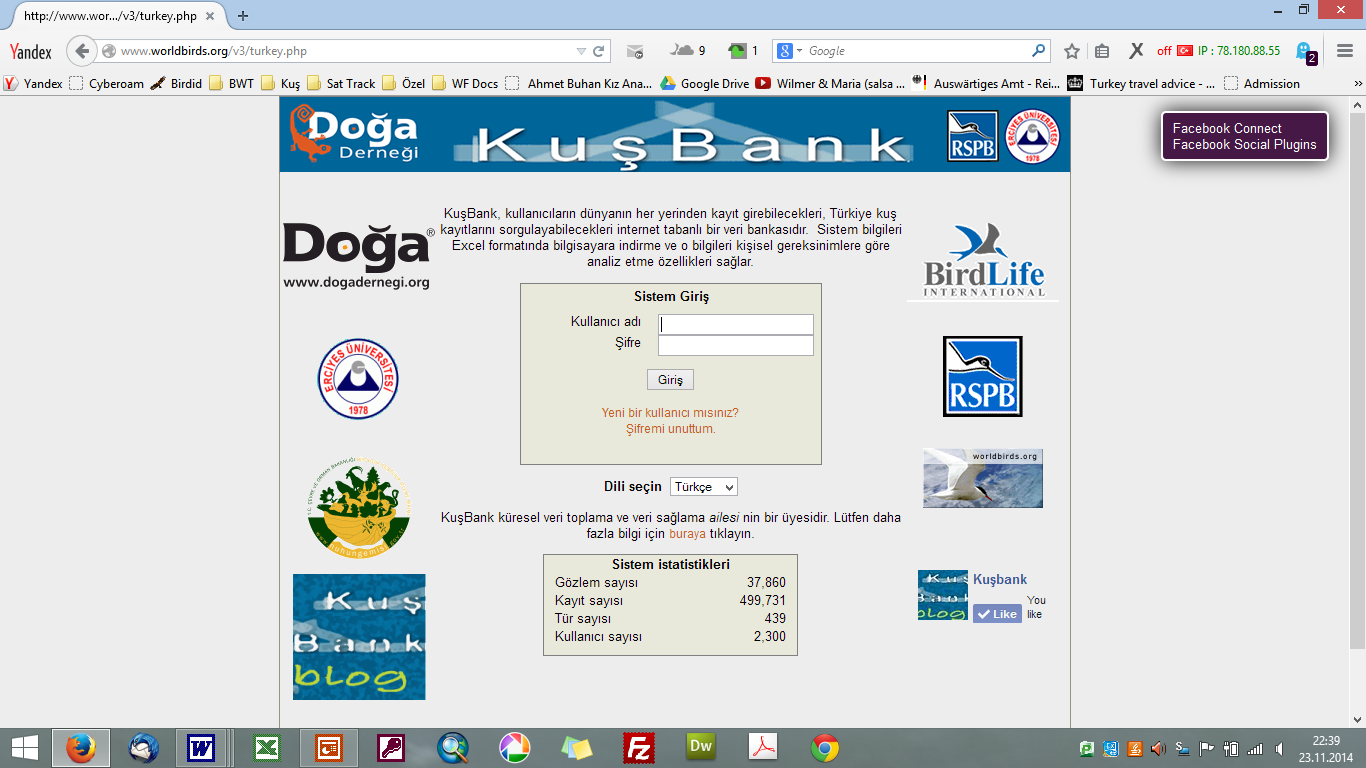
\includegraphics{images/kusbank.png}

}

\caption{KuşBank internet sitesinin ilk hali. Bugün ebird.org olarak
devam etmektedir.}

\end{figure}%

\section*{TRAKUS ve Kuş
Fotoğrafçılığı}\label{trakus-ve-kuux15f-fotoux11frafuxe7ux131lux131ux11fux131}
\addcontentsline{toc}{section}{TRAKUS ve Kuş Fotoğrafçılığı}

\markright{TRAKUS ve Kuş Fotoğrafçılığı}

Türkiye'de doğa fotoğrafçılığı alanında önemli bir gelişme, kuş
fotoğrafçılığına ilgi duyan bir topluluğun oluşmasıdır. 2007 yılında kuş
fotoğrafçıları ve kuş gözlemcileri için paylaşım platformu olarak
kurulan www.trakus.org internet sitesi üyelerinin katkılarıyla, kuş
fotoğraflarının çekilmesine adanmış gönüllüler, yer ve zaman bilgisiyle
desteklenen çok sayıda kuş fotoğrafını paylaşarak benzersiz bir veri
kaynağı oluşturdular. Nadir veya sadece belirli yerlerde görülen
türlerin fotoğraflanması, ulusal düzeyde kuş turizmi ve rehberliğini
destekleyerek veri kapsam ve niteliğini artırdı. Bu sayede Ak Kaşlı
Çinte, Mahmuzlu Çinte, Uzun Kuyruklu Korsan Martı gibi nadir türler
kayıt altına alınırken, Balık Baykuşu ve Paçalı Baykuş gibi türlerin
üreme davranışları da doğrulanabildi. 2024 yılında yaklaşık 25 kişilik
gönüllü bir ekibin yıllarca süren çalışması sonucunda, Türkiye'de
bulunan kuş türlerini özgün fotoğraflarından tanıtan ve bu anlamda
``ilk'' olma özelliği taşıyan ``TRAKUS Türkiye'nin Kuşları'' kitabı
hazırlanmıştır.

\begin{figure}[H]

{\centering 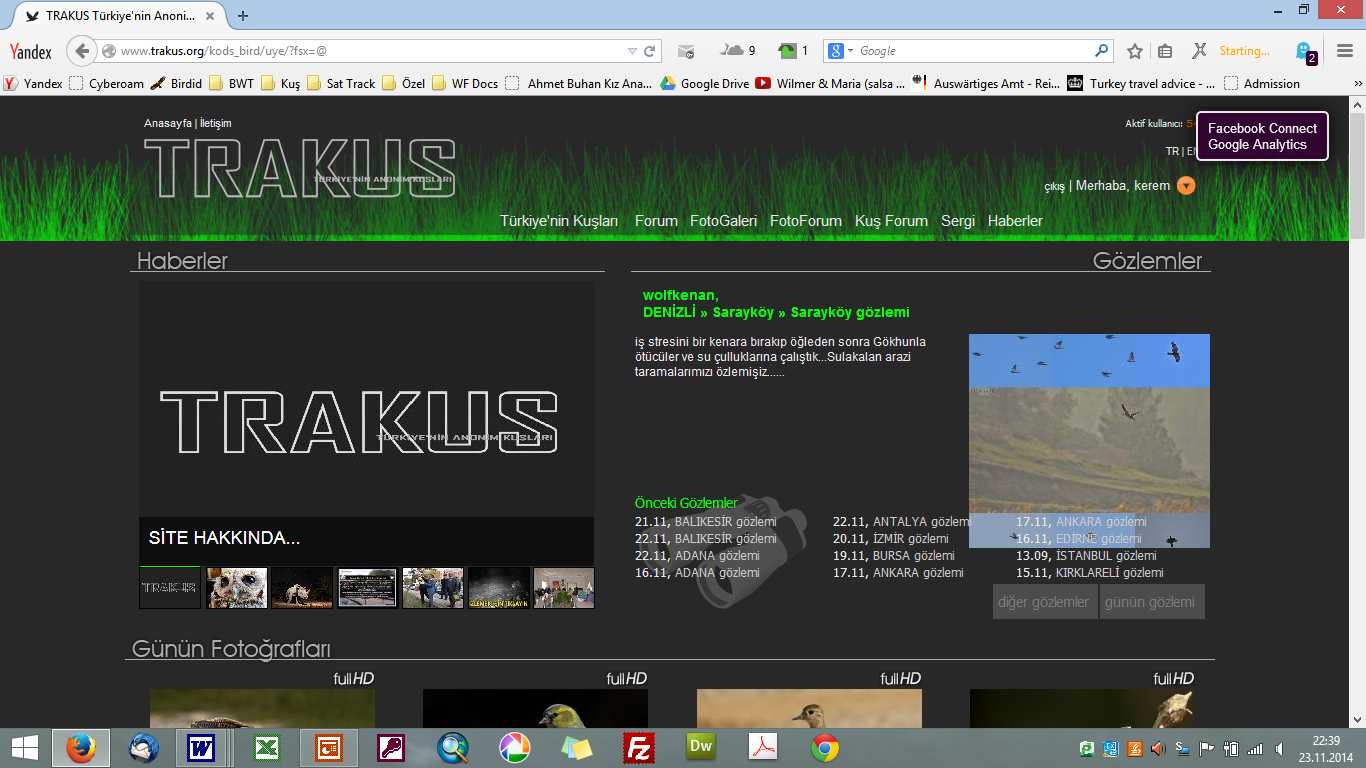
\includegraphics{images/trakus.png}

}

\caption{TRAKUS portalı. http://www.trakus.org}

\end{figure}%

\section*{Halkalama}\label{halkalama}
\addcontentsline{toc}{section}{Halkalama}

\markright{Halkalama}

Ötücü kuşlar ve yağmurcunların halkalanması, Türkiye'de ilk kez WIWO'nun
Çukurova (Kivit et al., 1994) ve Kızılırmak Deltası (Hustings and Dijk,
1994) projeleriyle başlamış olup, 2002 yılında ulusal halkalama
programının başlatılmasıyla Ankara, Manyas, Manavgat, Kars, Diyarbakır
ve Kızılırmak Deltası gibi alanlarda ilkbahar ve sonbahar dönemlerinde
halkalama yapılmaya başlanmıştır. Programdaki en eski ve sürekli çalışan
istasyon, Kızılırmak Deltası'ndaki Cernek Halkalama İstasyonu'dur (Barış
et al., 2005). Zamanla bazı istasyonlar düzenli çalışmasa da Kızılırmak
Deltası, Kars ve Antalya'da halkalama çalışmaları devam etmektedir.
Uluslararası projeler kapsamında su kuşlarının kuş gribine katkısını
araştırmak amacıyla su kuşları halkalanmış, örneklenmiş ve bazı bireyler
uydu vericileriyle takip edilmiştir. Ayrıca 2003-2009 yılları arasında
İzmir Tuzla'da yapılan beş flamingo halkalama çalışması, Akdeniz'deki
flamingo popülasyonlarına dair önemli veriler sağlamıştır (Balkız et
al., 2009).

\bookmarksetup{startatroot}

\chapter*{Bilgi Kaynakları ve
Boşlukları}\label{bilgi-kaynaklarux131-ve-boux15fluklarux131}
\addcontentsline{toc}{chapter}{Bilgi Kaynakları ve Boşlukları}

\markboth{Bilgi Kaynakları ve Boşlukları}{Bilgi Kaynakları ve
Boşlukları}

Hazırlayanlar: Geoff Welch, Hilary Welch and Sancar Barış (2005)

1990 ile 2005 yılları arasında, Türkiye'nin kuşları hakkındaki
bilgilerimiz, yerel kuş gözlemciliğinin ve doğa koruma topluluklarının
gelişmesine paralel olarak önemli ölçüde ilerlemiştir. Bu bölüm,
Türkiye'nin kuşlarıyla ilgili bilgimizi sınırlayan, bazıları genel
bazıları ise oldukça spesifik olan temel sorunları tanımlarken aynı
zamanda geleceğe yönelik olarak Türk kuş faunasına dair atılabilecek
önemli adımları ortaya koymaktadır.

\section*{Türlerin Yayılışı}\label{tuxfcrlerin-yayux131lux131ux15fux131}
\addcontentsline{toc}{section}{Türlerin Yayılışı}

\markright{Türlerin Yayılışı}

Gözlem haritaları, Kuşların yayılışı mı, yoksa kuş gözlemcilerinin mi?
Yakın zamana dek, Türkiye kuş veri havuzu büyük ölçüde tatil için Batı
Avrupa'dan gelen kuş gözlemcilerinin katkılarıyla oluşuyordu. Ülkeyi
ziyaret eden yabancı gözlemciler, kısa süreli tatilleri boyunca mümkün
olduğunca çok tür ve çeşitli yaşam ortamı görmek isterler. Bu durum
önemli ölçüde taraflı bir veri oluşturur; çünkü gözlemciler her zaman
aynı yerlere, yılın aynı dönemlerinde giderek hep aynı kuş türlerini
gözlemler.

Türkiye'de kuş gözlemciliğinin gelişmesiyle bu sıkıntı büyük ölçüde
azalmıştır. Ancak bu kez de yerli kuş gözlemcilerinin gözlem alanları
genellikle yaşadıkları bölgeyle sınırlı kalmakta; bu durum, veri
toplamada daha geniş bir yelpazeye ulaşmak adına farklı yöntemlerin
geliştirilmesi gerekliliğini doğurmaktadır.

\section*{Standart Verinin
Eksikliği}\label{standart-verinin-eksikliux11fi}
\addcontentsline{toc}{section}{Standart Verinin Eksikliği}

\markright{Standart Verinin Eksikliği}

1998 ile 2003 yılları arasında Türkiye'nin geniş alanlarında, standart
yöntemlerle üreyen kuşlar hakkında veri toplayan üç önemli proje
yürütülmüştür: Konya Havzası'nda (Eken \& Magnin 1999), Akdeniz
ormanlarında (Zeydanlı ve ark. 2005) ve Güneydoğu Anadolu'da (Welch
2004). Bu çalışmalar sayesinde, ilk kez, araştırma alanları nadir
türlerin varlığı ya da kuşların yoğunlaştığı alanlar gibi önceki
bilgilere bağlı kalınmadan tarafsız bir şekilde belirlenmiştir. Elde
edilen veriler kuşların kesinlikle nerelerde bulunduğunu göstermenin
yanı sıra neredeyse nerelerde bulunmadıklarını da ortaya koymuştur.
Ancak, bu tür çalışmalar önemli ölçüde daha fazla insan gücü gerektirir,
organize edilmesi zordur ve nispeten pahalıdır.

Yaygın türlerin yayılışı, gözlemcilerin bilinçsizce her yerde var
olduklarını düşündükleri kargalar, toygarlar, serçeler, sığırcıklar ve
evcil güvercinler gibi kuşları yeterince kaydetmemelerinden dolayı eksik
kalmaktadır. Örneğin, kumru her yerde bulunduğu varsayılan, hareket
halindeki bir araçtan bile kolayca gözlemlenebilecek bir tür olarak
bilinir. Ancak 2005 yılında ülkenin kuzeybatısında yapılan iki haftalık
saha çalışmasında Erzurum'un kuzeyinde bulunmadığı, Kars'ta hiç
kaydedilmediği ve ancak Yeşilırmak ovasında tekrar ortaya çıktığı tespit
edilmiştir.

\section*{Üreme Durumu}\label{uxfcreme-durumu}
\addcontentsline{toc}{section}{Üreme Durumu}

\markright{Üreme Durumu}

Kızıl Sırtlı Örümcekkuşu, Türkiye'deki kuşların yayılışının gözlem
verileriyle nasıl doğrulandığına iyi bir örnek teşkil eder. Bu tür, göç
dönemlerinde oldukça yaygın görülür ve çoğu kuş kitabı ile arazi
rehberinde Türkiye'nin geniş bir alanında üreyen bir tür olarak
tanıtılır. Ancak bu gerçekten böyle mi? Kızıl Sırtlı Örümcekkuşu'nun
(göç başlangıç ve bitiş tarihleri tam olarak belirlenemeyen) uzun bir
göç dönemi vardır. Ağustos 2005 itibarıyla Kuşbank veritabanındaki 313
kaydın 128'i (\%41) bir üreme koduyla ilişkilendirilmişken, yalnızca
yedisinde (\%2) kesin üremeye dair itiraz edilemez kanıt bulunmaktadır.
Geriye kalan 121 kaydın büyük bir kısmı, özellikle de 35 tanesi dışında
olanlar, muhtemelen göç eden bireylere aittir. Bazı durumlarda birkaç
dakikalık bir gözlem, ``olasılık'' düzeyinde bir üreme kaydını
``muhtemel'' veya ``kesin'' üreme kaydına dönüştürebilir.

\section*{Su Kuşu Sayımları}\label{su-kuux15fu-sayux131mlarux131}
\addcontentsline{toc}{section}{Su Kuşu Sayımları}

\markright{Su Kuşu Sayımları}

1986'dan itibaren IWRB/Wetlands International tarafından organize edilen
Kış Ortası Su Kuşu Sayımları (KOSKS), Türkiye'de uzun süreli su kuşu
verisi sağlamakta önemli bir rol oynamıştır. Ancak, bu program on
yıllardır sürdürülse de sayım metodolojisinde çeşitli değişkenlikler
gözlenmiştir: ziyaret edilen alanların sayısı, her bir alanın kapsanma
şekli, katılımcı sayısı ve deneyim seviyeleri yıllar içinde değişmiştir.
Bu yüzden, kışlayan kuş sayılarındaki artış veya azalışı incelemek için
yapılan çalışmalarda veri toplama yöntemindeki bu değişikliklerin de
dikkate alınması gerekmektedir. Belirli bir türün sayısındaki değişim,
gerçekten popülasyon artışına ya da azalmasına mı işaret etmektedir,
yoksa bu farklı yıllarda sayılan alanların kapsamı mı değişmiştir? Söz
konusu türün tespit zorluğu, alanların bazı yıllarda daha detaylı ya da
yüzeysel sayılması, sayım sonuçlarını etkileyebilir. Ayrıca, Türkiye
veya Doğu Avrupa-Rusya-Orta Asya'daki hava koşulları ve avcılık baskısı
gibi kontrol edilemeyen değişkenler de kuşların dağılımını
etkileyebilir.

2012 yılında kurulan Ulusal KOSKS Kurulu, bu sayımları daha kapsamlı ve
standart hale getirmeyi hedeflemiştir. Sayım yapılacak alanların
kapsamı, önemi ve isimlendirilmesi standartlaştırılmış; sabit sayım
istasyonları belirlenmiştir. Tüm metotlar ve protokoller, formlar ve
haritalarla birlikte kullanıma sunulmuştur. Ayrıca gözlem verilerinin
sistematik olarak Kuşbank'a kaydedilmesi, verilerin doğruluğunu
sağlamakla birlikte raporlamayı da kolaylaştırmıştır. KOSKS Kurulu daha
sonra dağılmıştır.

Bir alanı kullanan kuş sayısının mevsimden mevsime veya yıldan yıla
değişim göstermesi doğal bir durumdur. ÖKA (Önemli Kuş Alanı) olarak
belirlenmesi gereken bir alan, kötü bir yılda gözden kaçabilir veya
komşu alanlarda normalin dışındaki su seviyeleri nedeniyle geçici olarak
yüksek sayıda kuş barındırabilir. Bu tür durumlar, yalnızca sulakalanlar
ağındaki işleviyle önemli olan bir alanın, koruma açısından en öncelikli
yerlerden biri olarak değerlendirilmesine yol açabilir.

\section*{Gözden Kaçan Türler}\label{guxf6zden-kauxe7an-tuxfcrler}
\addcontentsline{toc}{section}{Gözden Kaçan Türler}

\markright{Gözden Kaçan Türler}

Bazı kuşlar daha çok dikkat çekerken bazıları ise gözlenmeden
varlıklarını sürdürebilir. Gececil kuşlar özel teknikler kullanılmadıkça
olduğundan daha az kayda geçer. Saklanan ve ürkek türler bolca
bulunmalarına rağmen fark edilmeyebilir. Örneğin, Paçalı Baykuş, aslında
Türkiye'de nispeten yaygın olabilecek bir türdür, ancak 25 yıl öncesine
kadar hiç kaydedilmemiştir.

Koloni halinde üreyen türler, uygun yaşam alanı bulsalar bile düzensiz
bir dağılım sergileyebilirler. Bazı türler ise erişilmesi zor, uzak
bölgelerde yaşadığından tespiti zorlaşır. Koloniler bir kez
keşfedildiğinde popülasyonu izlemek kolaylaşsa da, yeni koloniler bulmak
zorludur. Örneğin, İspir'deki kızıl akbaba kolonisi, yola yakın
kayalıklarda bulunduğu için bilinirken, komşu vadilerdeki potansiyel
koloniler hakkında bilgi yoktur.

Alpin türler genellikle parçalı bir yayılış gösterir, düşük yoğunlukta
bulunurlar ve bölgede kısa süre kalabilirler. Bu nedenle, yükseklerde
yaşayan kuşların dağılımını yeterince bilmek güçtür.

Kuş türlerinin seslerinden tanınması ise ayrı bir zorluk sunar.
Türkiye'deki kuş gözlemcileri ötüşle tanıma konusunda nispeten az
deneyimlidir. Ayrıca, bölgesel alttür ve ırkların ötüşleri hakkında
bilgi eksikliği de bulunur. Türkiye'de üreyen Kızılkuyruk, deneyimli
Avrupalı gözlemciler tarafından bile bazen Şakrak ile karıştırılır. Boz
Kirazkuşu gibi türler de ötüşleriyle benzer türlerle karışabilir ve
yaygın oldukları bölgelerde gözden kaçabilirler.

\section*{Popülasyon Tahminleri}\label{popuxfclasyon-tahminleri}
\addcontentsline{toc}{section}{Popülasyon Tahminleri}

\markright{Popülasyon Tahminleri}

Batı Avrupa'da her tür için güvenilir, bazen oldukça kesin popülasyon
rakamları mevcut olup, bu veriler koruma eylemlerinin uygulanmasına ve
Avrupa Birliği düzeyinde uzun vadeli koruma politikalarının
geliştirilmesine katkı sağlamaktadır.

Türkiye'de ise güvenilir kalitatif bilgiler ya çok sınırlıdır ya da eski
kalmıştır. Ülkenin genişliği, sınırlı sayıda yerli kuş gözlemcisinin
varlığı ve yurt dışından gelen gözlemcilerin aksine sistematik
araştırmalara katılmak için deneyim, zaman, finansal kaynak ve seyahat
imkanı kısıtlılığı, gözlemcilerin çalışmalarını zorlaştırmaktadır.
Akademik düzeyde kuşlarla ilgili ilgi ise oldukça yenidir ve yalnızca
birkaç tane uluslararası standartlarda yüksek lisans ve doktora tezi
tamamlanmıştır.

Toy, Leylek, Kara Akbaba ve Dağ Horozu gibi yüksek koruma değerine sahip
türler için çeşitli araştırmalar yapılmakta veya devam etmektedir. Bu
çalışmalarda, halktan gelen bilgiler (Leylek), radyo vericileriyle
izleme (Kara Akbaba) ve bilgisayar destekli modellemeler (Dağ Horozu)
gibi farklı yöntemler kullanılmaktadır. Ancak çoğu tür için yalnızca
``en iyi tahmin'' düzeyinde verilere sahibiz. Türkiye'de, Birecik'teki
yarı evcil kelaynak kolonisi haricinde, hiçbir tür için güvenilir
popülasyon tahmini bulunmamaktadır.

Kuş gözlemcileri için sulakalanlar, kuş çeşitliliği ve gözleme kolaylığı
nedeniyle cazip alanlardır ve gözlemlerden elde edilen kayıtların çoğu
bu alanlardan gelmektedir. Ancak, yıllar içinde bu sulakalan odaklı
gözlem eğilimi, Devlet Su İşleri'nin 1930'lardaki master planlara uygun
olarak sulakalanları kurutup baraj inşa etmesiyle, hızla kaybolan türler
ve habitatlar listesine dönüşmüştür.

\section*{Göç Sayımları}\label{guxf6uxe7-sayux131mlarux131}
\addcontentsline{toc}{section}{Göç Sayımları}

\markright{Göç Sayımları}

Gündüz yırtıcılarının ve diğer süzülen kuşların görünür göçü Türkiye'de
uzun zamandır biliniyor olsa da, bu göçün sürdürülebilir ve eşgüdümlü
olarak izlenmesi için yapılan çalışmalar oldukça sınırlıdır. 1960'lar ve
70'lerde İstanbul Boğazı, Kuzey-Batı Türkiye ve İskenderun Körfezi'nde
gündüz yırtıcılarının ve süzülen kuşların gözlenmesi (Beaman, 1977;
Beaman and Porter, 1977; Porter and Willis, 1968; Sutherland and Brooks,
1981), batılı kuş gözlemcilerinin Türkiye'deki bu önemli göçün farkına
varmasını sağlamış ve büyük bir ilgiyle Türkiye'yi ziyaret etmelerine
vesile olmuştur.

Görülebilir göç sayımı, uzun süreli yoğun konsantrasyon ve disiplin
gerektiren bir iş olup, kendini işe adamış az sayıda gözlemci tarafından
gerçekleştirilir. Bu nedenle, dünyada düzenli ve uzun süreli gündüz
yırtıcı göçü çalışmaları oldukça sınırlıdır. Ayrıca, elde edilen
verilerin koruma değerinin belirginleştirilmesi zor olduğundan, yırtıcı
sayımları için mali kaynak bulmak da kolay değildir. Yine de, süzülen
kuş göçü görsel açıdan oldukça etkileyici bir doğa olayıdır ve toplumun
doğal çevreye olan ilgisini ve korunma gereksinimine dair farkındalığını
artırmak için güçlü bir araçtır; bu nedenle, önemi göz ardı
edilmemelidir.

\section*{Halkalama İstasyonları}\label{halkalama-istasyonlarux131}
\addcontentsline{toc}{section}{Halkalama İstasyonları}

\markright{Halkalama İstasyonları}

Ötücü kuşlar ve yağmurcunların halkalanmasını içeren çalışmalar,
Türkiye'de ilk olarak WIWO'nun 1990'da Çukurova (Kivit et al., 1994) ve
1992'de Kızılırmak Deltası'nda (Hustings and Dijk, 1994) yürüttüğü
çalışmalarında başlamıştır. 2002 yılında ulusal halkalama programının
hayata geçirilmesiyle birlikte eğitimli halkalamacılar yetiştirilmiş ve
Ankara, Manyas, Manavgat, Kars, Diyarbakır ve Kızılırmak Deltası'nda
ilkbahar ve sonbaharda halkalama yapılan bir program oluşturulmuştur. Bu
programdaki en eski ve sürekli çalışan istasyon, Kızılırmak
Deltası'ndaki Cernek Halkalama İstasyonu olmuştur (Barış et al., 2005).

Bu tür çalışmaların uzun vadeli koruma açısından sağladığı en önemli
yarar, konaklama alanlarını kullanan kuş sayılarındaki değişimlerin ve
popülasyon hareketlerinin izlenmesine olanak tanımasıdır. Böylelikle her
alanın kuşlar açısından taşıdığı gerçek önem ortaya konulabilir. Sürekli
ve standart çalışan halkalama istasyonları, Türk ornitolojisine sadece
veri sağlamakla kalmayıp, uzun vadede daha kapsamlı katkılar
sunmaktadır.

\section*{Kuşbank ve eBird}\label{kuux15fbank-ve-ebird}
\addcontentsline{toc}{section}{Kuşbank ve eBird}

\markright{Kuşbank ve eBird}

Türkiye için elde edilen tüm bilgilerin erişilebilir ve koruma
çalışmalarına katkı sağlayacak bir formatta saklanması büyük önem taşır.
Bu amaçla, 2001 yılında kurulan ve 2004'te kullanıma açılan KuşBank
ağ-temelli veri tabanı geliştirilmiştir. KuşBank, kuş gözlemcileri
tarafından geniş kabul görmüş ve oldukça başarılı olmuştur. Kasım 2005
itibarıyla, veritabanına 350 gözlemci tarafından 400 türe ait 97.000'den
fazla kayıt girilmiştir. Ancak verilerin gerçek anlamda değerli
olabilmesi için kalite güvence altına alınmalıdır. Bu nedenle, belirli
standartların karşılandığından emin olmak amacıyla bir Kayıt Komitesi
oluşturulmuştur. Başlangıçta sadece KuşBank'a girilen kayıtları
değerlendiren bu komitenin, zamanla ulusal ölçekte nadir türlerin
kayıtlarını inceleyen bir komiteye dönüşmüştür.

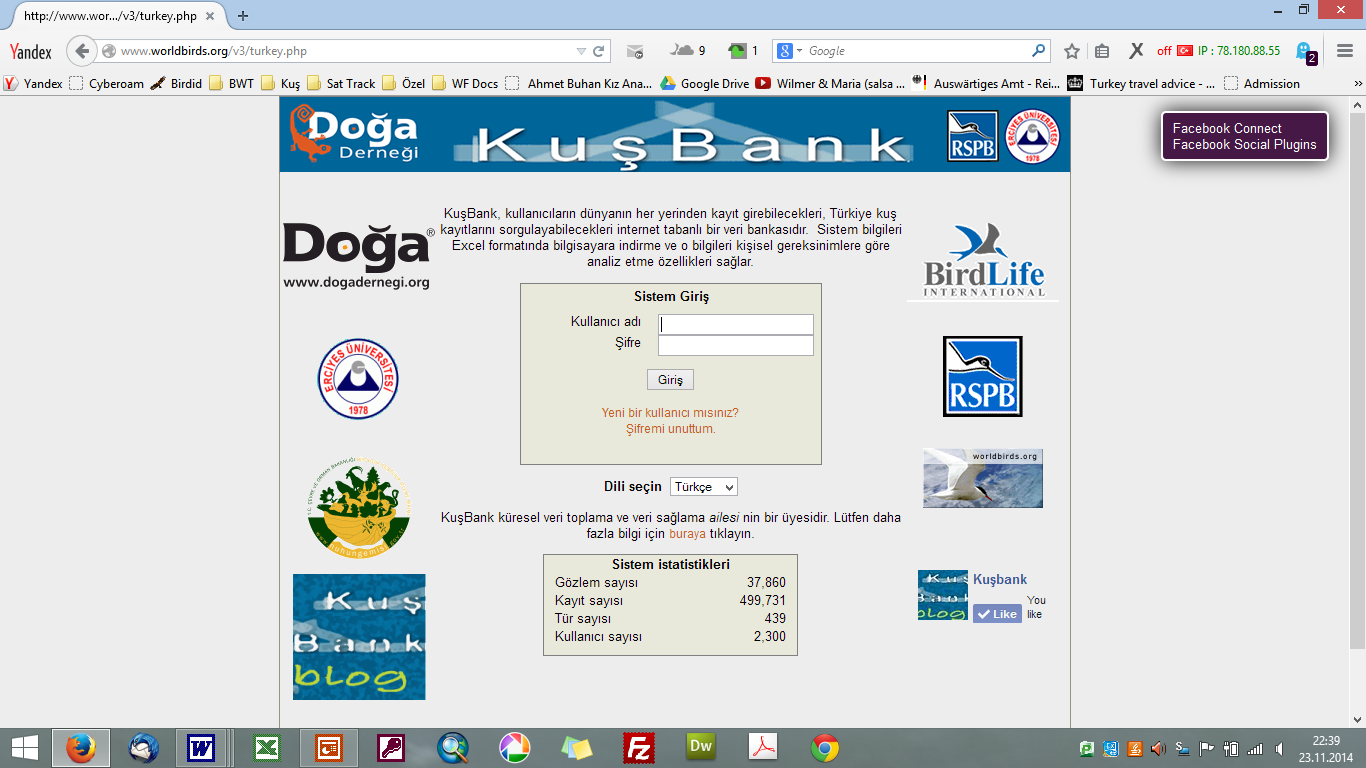
\includegraphics{images/kusbank.png}

\section*{Türkiye Üreyen Kuş
Atlası}\label{tuxfcrkiye-uxfcreyen-kuux15f-atlasux131}
\addcontentsline{toc}{section}{Türkiye Üreyen Kuş Atlası}

\markright{Türkiye Üreyen Kuş Atlası}

Türkiye kuşları hakkında yöntemselliğe dayalı nitelikli çalışmalar ve
güvenilir verilerle koruma önceliklerini belirleyebilme gereksinimi,
bugün hala aşılması gereken önemli bir sorun olarak karşımızda
durmaktadır. Türkiye'de yöntemsel çalışmaları bağımsız olarak
yürütebilecek kuş gözlemcilerinin sayısı yüz civarında olsa da,
metindeki tespitler ve eleştiriler geçerliliğini korumaktadır. Bu
bağlamda, kuş gözlemcilerinin katkılarının koruma çalışmalarına daha
etkili yansıması için stratejik yaklaşımlar geliştirilmesi önemlidir.
Koruma liderlerinin öncelikli alanlar, türler ya da veri eksikliklerini
sistematik olarak belirlemeleri ve giderek artan akademik kapasiteye
sahip üniversitelerle iş birliği yapmaları, kuş gözlemcilerinin veri
açıklarını kapatma konusunda daha verimli olmasını sağlayabilir. Kış
Ortası Su Kuşu Sayımları'nın analiz edilmesi, ulusal düzeyde bilgi
sağlayacak bir yaygın kuş gözlem programının yaygınlaştırılması ve
dinamik bir kuş atlasının oluşturulması hala gerçekleştirilmesi beklenen
adımlar arasında yer almaktadır.

Not: Bu yazı yazıldıktan sonra 2018 yılında Türkiye Üreyen Kuş Atlası
çalışması tamamlanmıştır!

\bookmarksetup{startatroot}

\chapter{Ördekgiller}\label{uxf6rdekgiller}

\section{Boz Kaz}\label{boz-kaz}

\emph{Anser anser}, Greylag Goose

\textbf{\emph{Lokal olarak az sayıda ürer. Kışın göç alır ve daha geniş
bir alanda yayılış gösterir.}}

Üreme döneminde az sayıda Göller Bölgesi, İç Anadolu ve Doğu
Anadolu'daki bataklık sulakalanlarda bulunur. Sultansazlığı gibi birkaç
alanda eskiden yüksek sayılarda üremiştir. Türkiye Kuş Raporları üreyen
popülasyonun son 50 yılda çok ciddi bir düşüş yaşadığını göstermektedir
(Beaman, 1986; Kirwan et al., 2009, 2003; Kirwan and Martins, 2000,
1994; Kirwan and Özen, 2014; Martins, 1989; OST, 1978, 1975, 1972,
1969). Eskiden ürediği sulakalanların çoğu kurutulmuştur. Örneğin,
Ereğli Sazlığı'nda Nisan 1970'te 120 yuva ve 300 birey varken Temmuz
1996'da 160 birey sayılmış, bugün ise hiçbir üreyen çift kalmamıştır.

Üreme sonrasında tüy dökümü sırasında kalabalık sürüler bazı
sulakalanlarda toplanır; Temmuz 1984'te Kulu Gölü'nde 800 birey,
bilinmeyen bir tarihte Sultansazlığı'nda 12.000 birey ve Eylül 2004'te
Kuyucuk Gölü'nde 10.000 birey kaydedilmiştir.

Geçiş sırasında tüm bölgelerde görülen ve ekimden itibaren mart sonuna
kadar kalan bir kış göçmenidir. Kışlayan sürüler genellikle kıyısal
bölgelerde yoğunlaşır. Son yıllarda görülen sürüler 300 bireyden azdır.
KOSKS verilerine göre eskiden daha bol bulunduğu bilinmektedir. Ülke
genelinde ortalama 5000 birey, en yüksek ise 1967'de 11.200 birey olarak
sayılmıştır. Alanlarda yapılan sayımlarda Kızılırmak Deltası'nda 5000
birey, Meriç Deltası'nda 4500 birey ve Hotamış Sazlığı'nda 1500 birey
tespit edilmiştir.

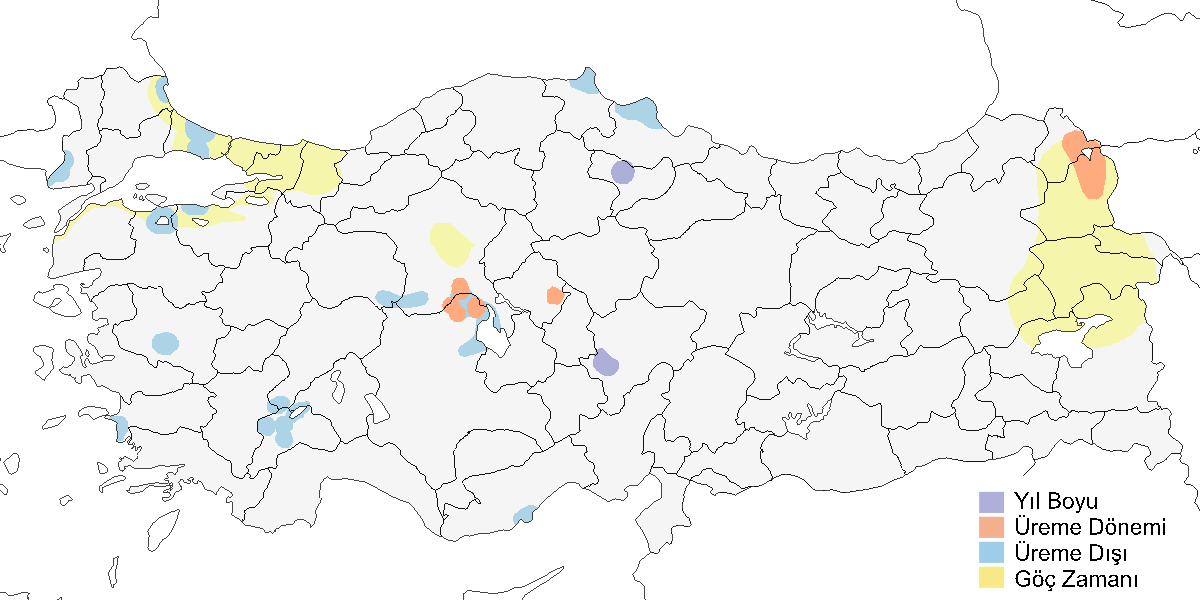
\includegraphics{images/harita_Anser anser.png}

\textbf{Üreme}

\textbf{Yuvalama Alanı:} Göllerdeki adalarda genellikle küçük gruplar
halinde ürer.\\
\textbf{Yuvası:} Kulu Gölü'nde gözlenen yuvası kuru toprağa kazılmış sığ
bir çukurdur ve çevredeki bitki örtüsü ile küçük tüylerle
astarlanmıştır. Ereğli Sazlığı'ndaki yuvası ise saz ve diğer sucul
bitkilerden oluşan, su seviyesinin üstünde kalan bir yapının üzerine
kurulmuştur.\\
\textbf{Yumurta Sayısı:} Türkiye'de yumurta sayısına ilişkin güvenilir
gözlem yoktur. Yuvadan ayrılmış beş yavru, en az beş yumurta koyduğunu
gösterir. Diğer ülkelerde genellikle 4-6 yumurta bırakır.\\
\textbf{Üreme Dönemi:} Mart sonunda yumurta koyar. En erken yavrular 23
Nisan 1988'de Kulu Gölü'nde, 27 Nisan 1988'de Sultansazlığı'nda, 30
Nisan 1968'de Mogan Gölü'nde ve 30 Nisan 1973'te Ereğli Sazlıkları'nda
gözlenmiştir. 20 Nisan 1996'da Marmara'da, 14 Mayıs 1969'da
Karadeniz'de, 16 Mayıs 1970'te ve 24 Haziran 1983'te Doğu Anadolu'da
kaydedilen yavrular gecikmiş üremeyi göstermektedir.

\textbf{Alttürler ve Sınıflandırma}

Ülkemizde \emph{rubrirostris} alttürü bulunur. Bu alttür turuncu
gagasıyla Batı ve Orta Avrupa'da bulunan pembe gagalı \emph{anser}
alttüründen ayrılır.

\section{Sakarca}\label{sakarca}

\emph{Anser albifrons}, Greater White-fronted Goose

\textbf{\emph{Lokal olarak bulunan ve zaman zaman kalabalık sürüler
oluşturan bir kış konuğudur.}}

Ekim sonu ile nisan başı arasında lokal olarak görülen bir kış
konuğudur. Genellikle ocak ve şubat aylarında daha yaygın ve yüksek
sayıda olur. Soğuk geçen kışlarda Türkiye'de kışlayan birey sayısı
artar. En kalabalık sürüler Meriç Nehri boyunca, Tuz Gölü çevresinde ve
Konya Ovası'nda yoğunlaşır. Büyük Menderes Deltası ve Doğu Akdeniz'deki
sulakalanlarda da önemli sayılarda toplanabilir. Son zamanlarda
Güneydoğu Anadolu'daki baraj göllerinde küçük sürüler halinde görülmeye
başlanmıştır. Nadiren yaz aylarında sulakalanlarda az sayıda birey
kalabilir.

Kış ortası su kuşu sayımlarında (KOSKS) ülke genelinde en yüksek sayı
1968-69 kışında 98.600 birey olarak kaydedilmiştir. 1987'de ise toplam
84.000 birey sayılmıştır. Ancak daha sonra kışlayan birey sayısında
ciddi bir düşüş yaşanmıştır. 1990'lı yıllarda genellikle 20.000-30.000
arasında değişen sayılar kaydedilmiş 1993'te 11.822 (DHKD, 1993),
1999'da 3956 (DHKD, 1999) ve 2005'te 3891 birey (Çağlayan et al., 2005)
tespit edilmiştir. Kışın soğuk geçtiği 11 Şubat 2006'da Büyükçekmece'de
15.000 birey sayılmıştır, bu da son yıllardaki en yüksek sayıdır.
Dolayısıyla Türkiye'de kışlayan nüfusun 1970'lerde 100.000'ler
seviyesinden 2010'larda 5000 civarına indiği söylenebilir.

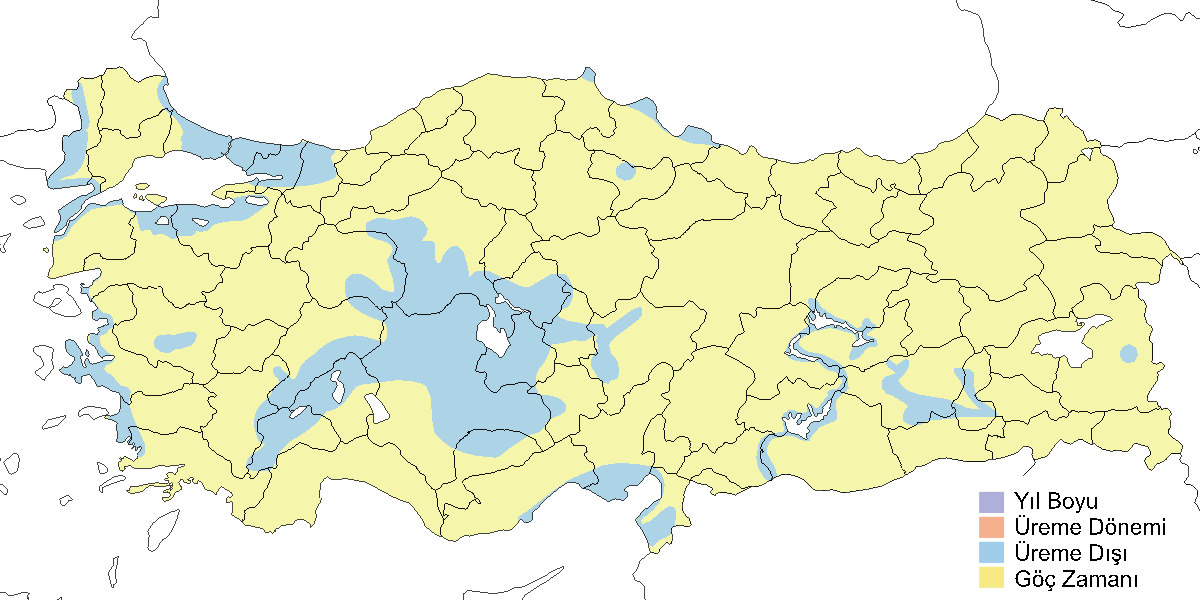
\includegraphics{images/harita_Anser albifrons.png}

\textbf{Üreme}

Türkiye'de yuvalamaz. Avrasya ve Kuzey Amerika'nın tundra bölgelerinde
yuvalar.

\textbf{Alttürler ve Sınıflandırma}

Türkiye'de nominat alttürü bulunur.

\section{Küçük Sakarca}\label{kuxfcuxe7uxfck-sakarca}

\emph{Anser erythropus}, Lesser White-fronted Goose

\textbf{\emph{Az sayıda gelen düzenli kış konuğudur.}}

Her yıl çok az sayıda kaydedilen bir kış konuğudur. Sayıları genellikle
10'dan azdır ve diğer kaz türleriyle karışık olarak görülebilir. Bugüne
kadar Türkiye'ye gelen bireylerin İskandinavya'da üreyen ve Balkan
ülkelerinde kışlayan göç yoluna ait olduğu düşünülmüştür. Yunanistan'da
bir alanda kışlayan ve koruma çalışmaları sayesinde sayıları artan bir
sürünün kış ortasında oradan kaybolması, Marmara ve Ege bölgelerinde bir
kışlama alanı olabileceği ihtimalini doğurmuştur. Ancak yapılan
aramalara rağmen burada düzenli kullanılan bir kışlama alanı
bulunamamıştır.

Doğu Anadolu'da 20 Kasım 2004'te Haçlı Gölü'nde uydudan izlenen bir
birey sinyal verince, doğuda bir kışlama alanı olasılığı gündeme
gelmiştir (Morozov and Aarvak, 2004). Nitekim Van Gölü ve Erçek Gölü
kıyılarında sayıları 340'a ulaşan sürüler düzenli olarak tespit
edilmiştir. Bugün, Türkiye'de kışlayan ana nüfusun Doğu Anadolu'da
bulunduğu söylenebilir ((AOU), 2000).

2000 öncesindeki kayıtlara bakıldığında; 29 Aralık 1997'de Göksu
Deltası'nda bir birey (Kirwan et al., 2003), 23 Ocak 1993'te Göksu
Deltası'nda bir birey (DHKD, 1993), 6 Nisan 1990'da Seyfe Gölü'nde 12
birey (Kirwan and Martins, 1994), 24 Aralık 1986'da Bafa Gölü'nde bir
erişkin ve iki genç birey (Kasparek, 1988) ve 16 Şubat 1967'de Kocabaş
Çayı'nın ağzında (Çanakkale) iki birey (OST, 1969) kaydedilmiştir. 1945
ile 1965 yılları arasında ve ekim ile ocak aylarında, çoğunluğu
Büyükçekmece ve Küçükçekmece Göllerinden gelen 12 kayıt vardır. Ancak bu
kayıtlar, tür tanımını destekleyecek belgeden yoksundur (Kumerloeve,
1970a).

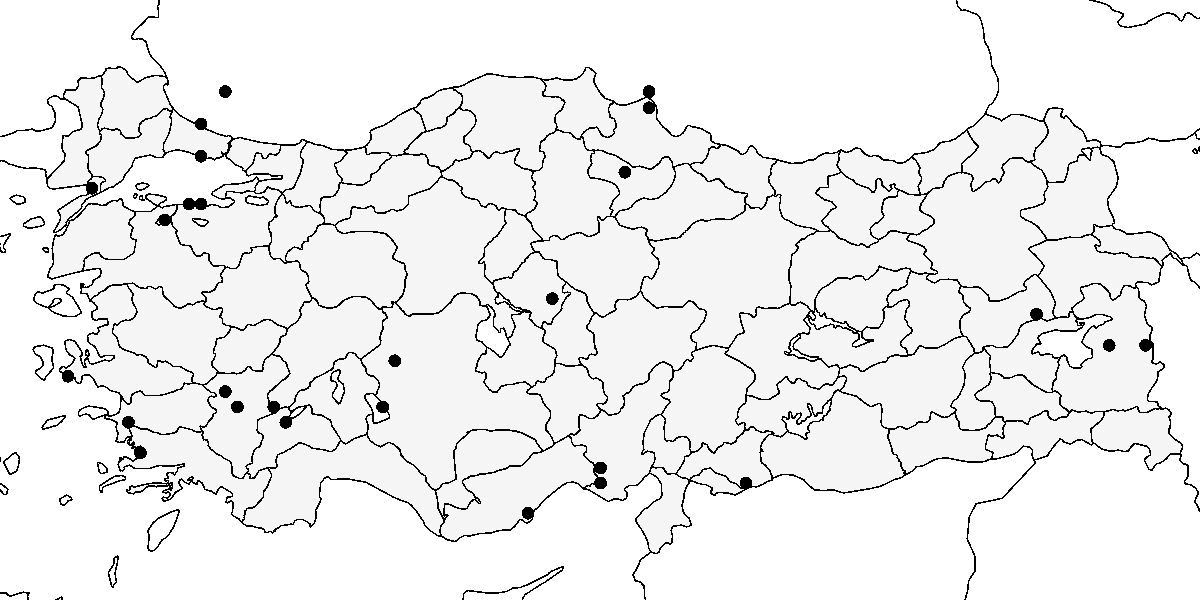
\includegraphics{images/harita_Anser erythropus.png}

\textbf{Üreme}

Türkiye'de yuvalamaz. Kuzey İskandinavya'dan Doğu Sibirya'ya kadar
uzanan tundra kuşağında ürer.

\textbf{Alttürler ve Sınıflandırma}

Monotipik bir türdür.

\section{Tundra Kazı}\label{tundra-kazux131}

\emph{Anser serrirostris}, Tundra Bean Goose

\textbf{\emph{Nadiren gelen kış konuğudur.}}

2000 yılından sonra 5 kez kaydedilmiştir. 26 Şubat 2013'te Yedikır
Barajı'nda, 4-21 Şubat 2015'te Kızılırmak Deltası'nda birer birey
görülmüştür. 31 Ocak 2016'da Manyas Kuş Gölü'nde 3 birey kaydedilmiş,
aynı alanda 2-24 Ocak 2019'da yine 3 birey gözlenmiştir. Acıgöl'de 24
Aralık 2023 ile 3 Şubat 2024 arasında bir birey gözlenmiştir.

\emph{Tundra Kazı}, önceleri \emph{Tayga Kazı} ile beraber tek bir tür
altında \emph{Tarla Kazı} olarak sınıflandırılıyordu. Dolayısıyla,
taksonomik revizyonun yapıldığı tarihten önceki kayıtlarda \emph{Tarla
Kazı} olarak tanımlanmıştır. 2000 yılından sonra çekilen fotoğraflarda
özellikle gaga renklenmesi incelenmiş ve bu kuşların tamamı \emph{Tundra
Kazı} olarak tanımlanmıştır. Fotoğrafı veya betimlemesi olmayan eski
kayıtların hangi türe ait olduğu ise belirsiz kalacaktır.

\emph{Tarla Kazı} olarak tanımlanmış kuşlar, Ege, Akdeniz ve İç
Anadolu'daki sulakalanlarda ara sıra yüksek sayılarda kaydedilmiştir.
1870'ler ve 1880'lerde Mersin'de toplanan bireyler (Schrader, 1891) ilk
kayıtlar arasındadır. 1966-2000 yılları arasında çoğunlukla ocak ile
mart ayları arasında 15 kez kaydedilmiştir. 2 Mart 1965'te Ereğli ve
Karapınar arasında 90 birey (Kumerloeve, 1970a), 15-16 Ekim 1969'da
Karamık Sazlıkları'nda 13 birey (OST, 1972), 30 Nisan 1988'de Seyfe
Gölü'nde, 30 Ocak 1992'de Marmara Gölü'nde 61 birey, 9 Ocak 1993'te
Büyükçekmece Gölü'nde 64 birey (DHKD, 1993) ve 24 Ocak 1993'te Göksu
Deltası'nda bir birey (DHKD, 1993) kaydedilmiştir. Türkiye'deki kışlayan
Sakarca sayılarındaki sert düşüş, muhtemelen \emph{Tarla Kazı} olarak
tanımlanmış kuşlar için de geçerlidir.

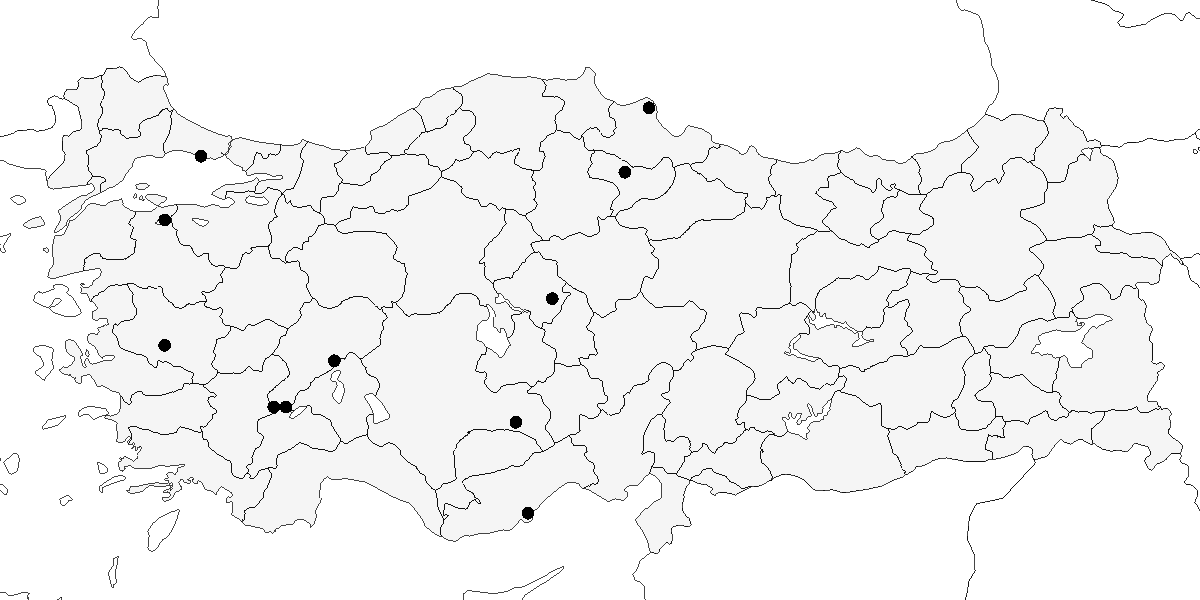
\includegraphics{images/harita_Anser serrirostris.png}

\textbf{Üreme}

Türkiye'de yuvalamaz. Üreme alanı Kuzey İskandinavya'dan Doğu Sibirya'ya
uzanan tundra kuşağındadır.

\textbf{Alttürler ve Sınıflandırma}

Tayga Kazı, yakın zamana kadar Tarla Kazı olarak bilinen bir türden
ayrılan yeni bir türdür. Beş alttüre sahip olan Tarla Kazı (\emph{Anser
fabalis}), iki gruba ayrılmıştır: \emph{fabalis}, \emph{johanseni} ve
\emph{middendorffii} alttürleri Tayga Kazı (\emph{Anser fabalis}),
\emph{serrirostris} ve \emph{rossicus} alttürleri ise Tundra Kazı
(\emph{Anser serrirostris}) olarak sınıflandırılmıştır.

\section{Yosun Kazı}\label{yosun-kazux131}

\emph{Branta bernicla}, Brant Goose

\textbf{\emph{Rastlantısal konuktur.}}

Batı Avrupa'nın Atlantik kıyılarında kışlayan bir türdür. Türkiye ile
yakın coğrafyasında rastlantısal bir konuktur. 6 Nisan 1981'de Küçük
Menderes Deltası'nda iki birey gözlenmiştir (Beaman, 1986). 3-4 Eylül
1973'te Ardeşen açıklarında koyu karınlı \emph{bernicla} alttürüne ait
iki birey kaydedilmiştir (OST, 1975). 1969 yılında Acıgöl'den gelen bir
iddia ise kabul edilmemiştir (Dijksen and Kasparek, 1988). 7 Şubat
1945'te Büyükçekmece'de bir birey Prenses Zeyneb Halim tarafından
vurulmuştur, ancak kuşun gövdesi korunamamıştır (Kumerloeve, 1970a).
Ocak 1889'da kışın soğuk geçtiği bir yılda İstanbul Maltepe'de düzenli
olarak, Şubat 1891'de ise büyük sürüler halinde İstanbul Kadıköy'de
görülmüştür (Mathey-Dupraz, 1920--24).

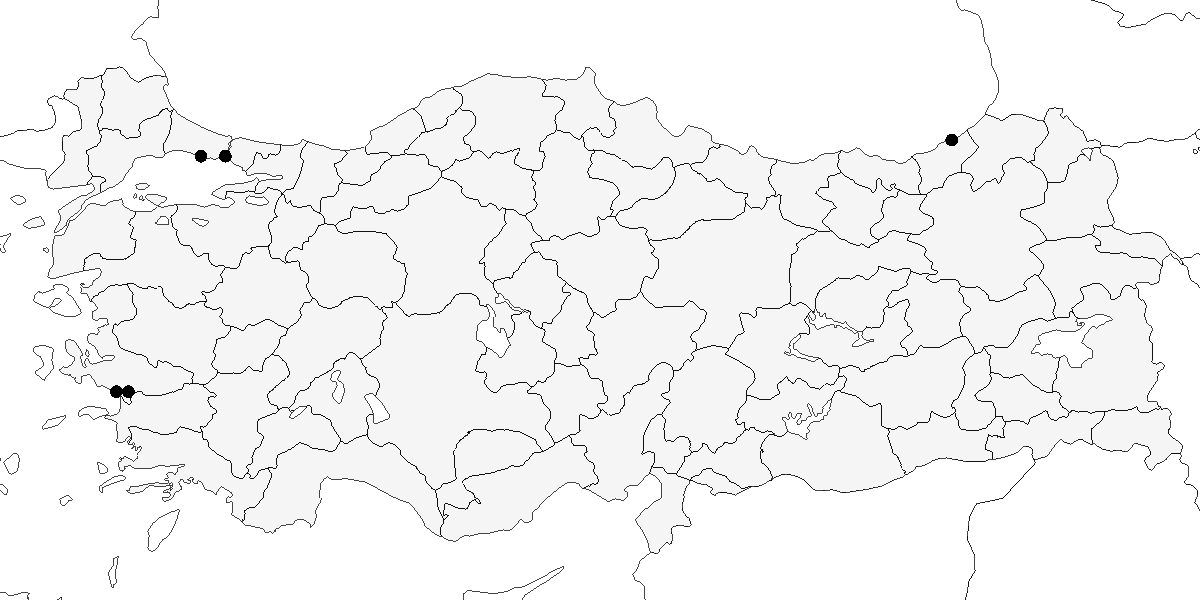
\includegraphics{images/harita_Branta bernicla.png}

\textbf{Üreme}

Türkiye'de yuvalamaz. Orta ve Kuzey Sibirya'nın Kutup Denizi kıyılarında
yuvalar.

\textbf{Alttürler ve Sınıflandırma}

Bir kayıtta kuşun alttürü \emph{bernicla} olarak tanımlanmıştır. Keza,
Kuzeybatı Avrupa'da kışlayan \emph{bernicla} alttürünün Türkiye'de
görülmesi olasıdır. Yunanistan'daki bir kayıt da bu alttüre aittir
(Handrinos and Akriotis, 1997).

\section{Ak Yanaklı Kaz}\label{ak-yanaklux131-kaz}

\emph{Branta leucopsis}, Barnacle Goose

\textbf{\emph{Rastlantısal konuktur.}}

5 Ocak 2003'te Büyükçekmece Gölü'nde bir birey gözlenmiş ve detaylı
olarak belgelenmiştir. 1946/47 kışında Sakarya Deltası'nda bir birey,
1961 sonbahar/kışında ise başka bir birey vurulmuştur. İkinci kuşun
tahniti Eylül 1964'te Ankara'da bulunmuş, ancak sahibi tahniti satmaya
yanaşmamıştır (Kumerloeve, 1966). Bu iki kaydın belgeleri yetersizdir
(Kumerloeve, 1970a).

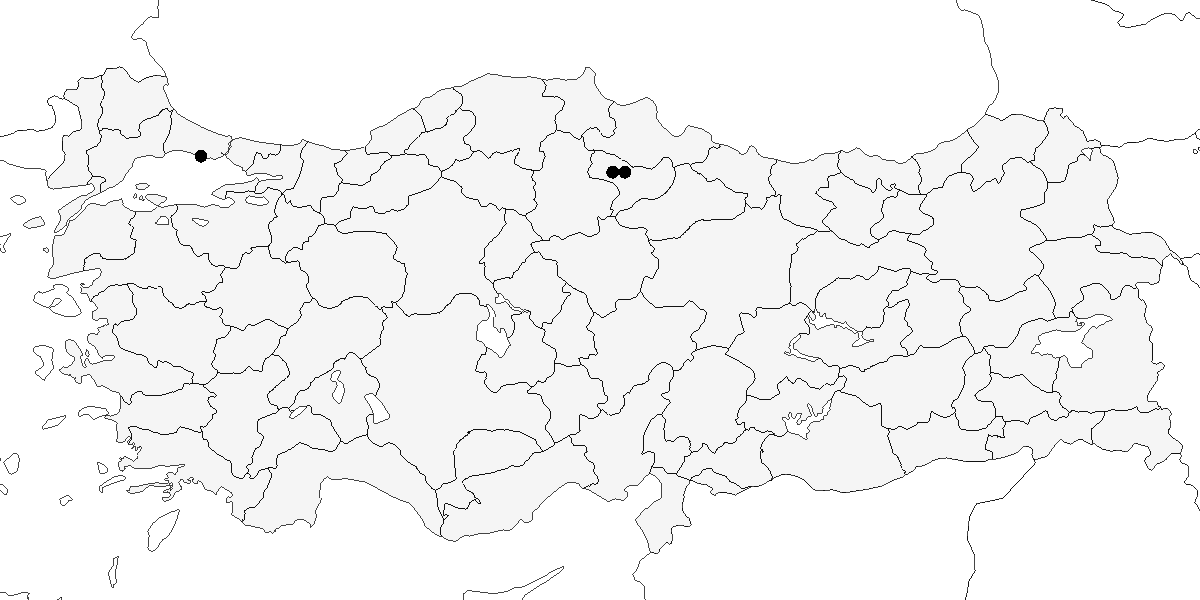
\includegraphics{images/harita_Branta leucopsis.png}

\textbf{Üreme}

Türkiye'de yuvalamaz. Grönland, İzlanda, Kuzey Batı Rusya ve Baltık
Denizi kıyılarında yuvalar.

\textbf{Alttürler ve Sınıflandırma}

Monotipik bir türdür.

\section{Sibirya Kazı}\label{sibirya-kazux131}

\emph{Branta ruficollis}, Red-breasted Goose

\textbf{\emph{Az sayıda gelen düzensiz kış konuğudur.}}

Türkiye'de düzenli kışladığı bilinen bir alan yoktur; ana kışlama alanı
Romanya ve Bulgaristan'ın Karadeniz kıyısıdır. Özellikle soğuk kışlarda,
bireyler veya gruplar halinde Türkiye'ye inerler. 1964 ile 2008 yılları
arasında 64 kayda rastlanmıştır. Bu kayıtların 15'i Marmara'da, 12'si İç
Anadolu'da, 8'i Karadeniz'de, 6'sı Akdeniz'de ve 4'ü Ege'de alınmıştır.
Kayıtların çoğu aralık sonu ile şubat başı arasındadır. Çoğunlukla bir
veya birkaç kuş sayılmış, ancak 5 kayıtta 40 ila 100 bireyden oluşan
nispeten kalabalık sürüler de gözlenmiştir. 2001/2002 kışında Türkiye
genelinde 192 birey sayılmıştır.

Ülke genelinde yaygın olarak av mağazaları ve avcılık kulüplerinde
tahnit örneklerine rastlanması ve avcıların gözlem beyanları (Dijksen
and Kasparek, 1985), bu kuşların kayıtlardan daha yaygın olabileceğini
gösterir. İç Anadolu'dan gelen eski kayıtlar, Kış Ortası Su Kuş
Sayımları sırasında kalabalık kaz sürülerinin sistematik incelenmesi ile
ortaya çıkmıştır. Sakarca kazı sürüleri içinde bu türün fark edilmemesi
olasıdır.

1946/47 kışında Küçükçekmece'de Kosswig tarafından gözlenmiştir
(Kumerloeve, 1966). 1947 veya 1954 yıllarında kış boyunca (27 Kasım - 6
Mart) Büyükçekmece ve Meriç Nehri civarında düzenli olarak 9 birey ve
Beylik Mandra'da 2 birey kaydedilmiştir (Kumerloeve, 1970a). 1959
yılında belirtilmemiş bir alanda İshakoğlu tarafından sekiz birey
gözlenmiş ve bir birey vurulmuştur (Makatsch, 1950). 12 Kasım 1964'te
Kuyucuk Gölü'nde 400 boz kazın arasında 2 erişkin ve 1 genç birey
kaydedilmiştir (Kumerloeve, 1964). 17 Ocak 1965 tarihinde Çekmece'de E.
Hirzel tarafından 3 birey görülmüştür.

Türkiye'de açıklama gerektiren bir yaz veya üreme kaydı vardır. 5
Ağustos 1982'de Erçek Gölü'nde 14 erişkin ve 8 yavru kaydedilmiştir
(Kasparek and Ven, 1983). Bu kayıt ya hatalı bir gözlem olarak kabul
edilmeli ya da avcılar tarafından yakalanıp evcilleştirilen kuşların
üremesinin bir sonucu olarak yorumlanmalıdır.

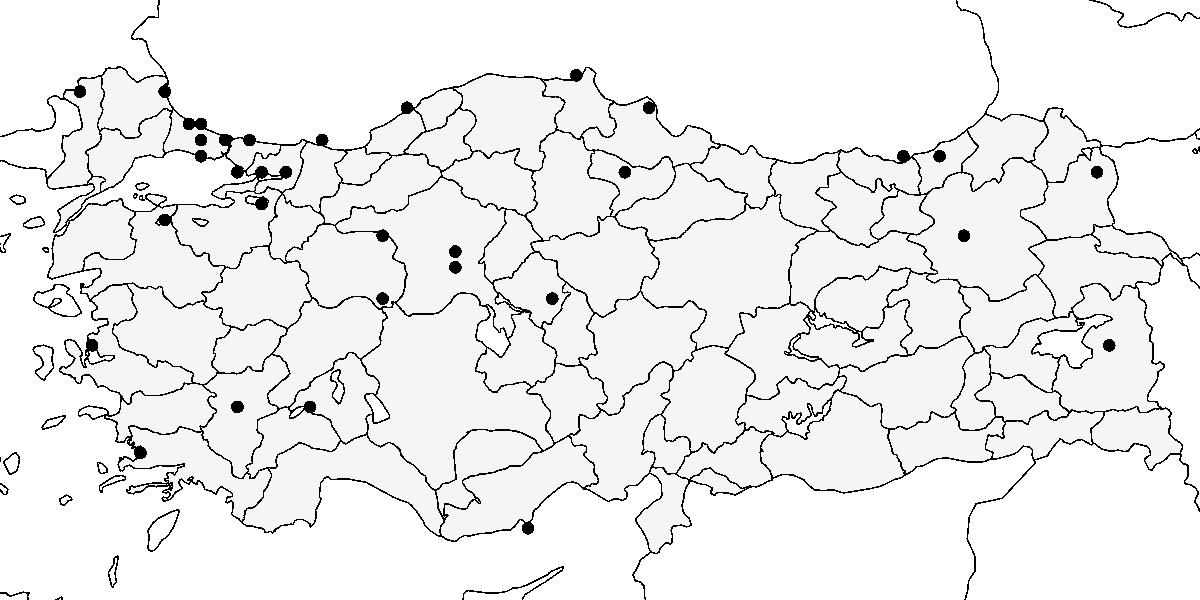
\includegraphics{images/harita_Branta ruficollis.png}

\textbf{Üreme}

Türkiye'de yuvalamaz. Doğu Sibirya'da tundra kuşağında yuvalar.

\textbf{Alttürler ve Sınıflandırma}

Monotipik bir türdür.

\section{Sessiz Kuğu}\label{sessiz-kuux11fu}

\emph{Cygnus olor}, Mute Swan

\textbf{\emph{Lokal olarak az sayıda yuvalar. Yaygın olarak ve nispeten
çok sayıda bulunan bir kış konuğudur.}}

Üreme kayıtlarının çoğu üç alandan gelir: Gala Gölü, Gediz Deltası ve
Kızılırmak Deltası. Ulusal üreme popülasyonu muhtemelen 20 çiftten daha
azdır. Kızılırmak Deltası'ndan alınan ilk muhtemel üreme kaydı 1968
yılına aittir (Dijksen and Kasparek, 1985).

Geçmişte, birkaç alanda yüzlerce çiftlik bir üreme nüfusu bulunuyordu.
Marmara Gölü'nde 50 çift, Akşehir Gölü'nde ise 100 çift üremiştir
(Kumerloeve, 1961). Ereğli Sazlığı en çok gözlem kaydının alındığı
alandır. Lenz burada 1968'de 11 yuva, 1969'da bir yuva ve 1970'de üç
yuva bulmuştur. Ereğli Sazlığı'nın yok olması ayrıntılı olarak
belgelenmiştir (Kılıç and Kasparek, 1990), bu nedenle üreyen nüfusun
azalışı da gözlenmiştir. Eski üreme alanlarında yok olmasının başlıca
nedeni sulakalanların kurutulmasıdır.

Kış aylarında Karadeniz, Marmara ve Ege Bölgelerinde yaygın olarak en
yüksek sayılarda gözlenir. Toplam kışlama popülasyonu 1000-10000 birey
arasında değişmektedir. Meriç Deltası ve Gala Gölü kışlayan nüfusun
büyük kısmının toplandığı alanlardır. 1993'te 1244, 1999'da 8900 ve
2003'te 2000 birey kaydedilmiştir (DHKD, 1999, 1993). Kışın sert geçtiği
yıllarda bu sayı artmakta olup, 1999'da ülke genelinde toplamda 9088
birey kaydedilmiştir.

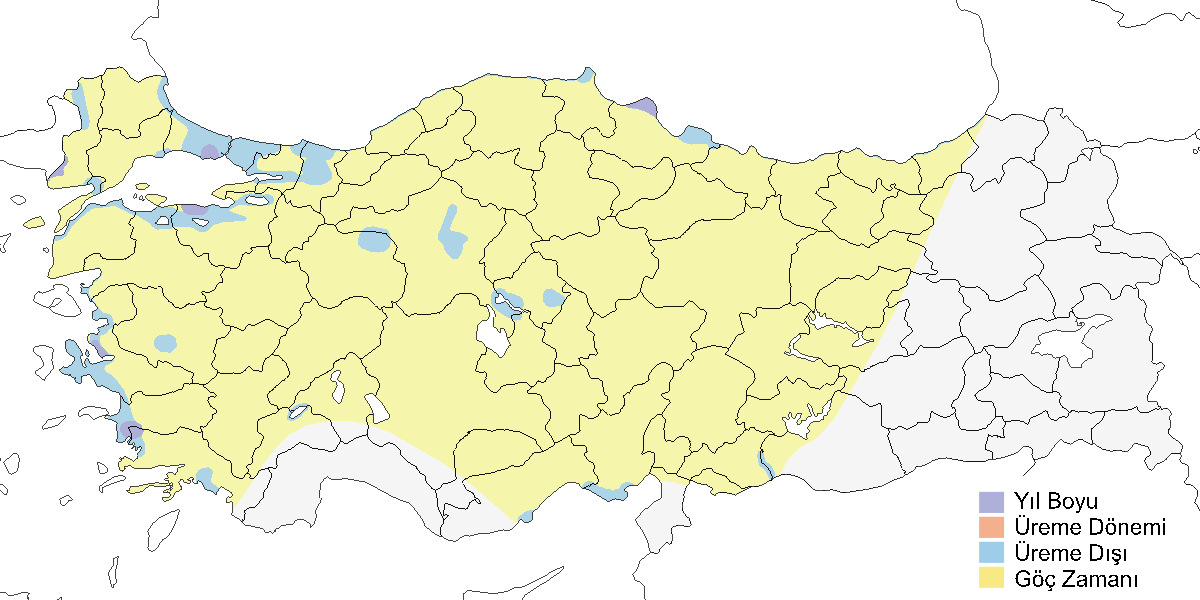
\includegraphics{images/harita_Cygnus olor.png}

\textbf{Üreme}

\textbf{Yuvalama Alanı:} Geniş sazlık alanlar, su aynası bulunan büyük
göller ve bataklıklarda yuvalar.\\
\textbf{Yuvası:} Türkiye'de henüz bir yuva tarifi yapılmamıştır. Diğer
bölgelerde yuva su kıyısındaki zemin üzerinde, küçük bir adacıkta ya da
sığ sudaki sazların üstüne kurulur. Yuva, saz ve diğer sucul bitkilerden
oluşan büyük bir yığının ortasında çukur şekilli bir yapıdır.\\
\textbf{Yumurta Sayısı:} Türkiye'deki yumurta sayısı bilinmez. Ancak
Türkiye dışındaki yuvalarda genellikle 5-7 yumurta bıraktığı
bilinmektedir.\\
\textbf{Üreme Dönemi:} Nisan başında yumurtlamaya başlar, yavrular ise
mayıs ve temmuz ayları arasında görülür. \textbf{EGE.} 13 Mayıs 1899'da
İzmir'de bir sazlıkta yuvalayan bir çift kaydedilmiştir (Selous, 1900).
\textbf{İÇA.} 6 Temmuz 1976'da Ereğli Sazlığı'nda bir çift ve 4-5 genç
yavru, 17 Temmuz 1982'de bir çift ve dört genç, 16 Mayıs 1987'de ise
yumurtadan yeni çıkmış yavrular gözlenmiştir.

\textbf{Alttürler ve Sınıflandırma}

Monotipik bir türdür.

\section{Küçük Kuğu}\label{kuxfcuxe7uxfck-kuux11fu}

\emph{Cygnus columbianus}, Tundra Swan

\textbf{\emph{Lokal olarak ve az sayıda bulunan bir kış konuğudur.}}

1993 yılına kadar nadir bir kış konuğu olduğu düşünülmüştür. Ancak daha
sonra, önce Burdur Gölü ve Göller Bölgesi'nde, ardından Meriç
Deltası'nda düzenli olarak bulunduğu tespit edilmiştir. Meriç
Deltası'nda, karışık ve kalabalık kuğu sürüleri içinde sayıları 1000'e
kadar ulaşabilir. İç Anadolu ve Göller Bölgesi'nde ise küçük gruplar
halinde bulunur. Genellikle kasım ve nisan ayları arasında gözlenir.

Türkiye'de kışlayan kuşların üreme alanları ve göç koridorları tespit
edilmiştir (Vangeluwe et al., 2018). 2015-2017 yıllarında GPS ve GMS
vericileriyle yapılan çalışmada, yuvalama alanlarının Yamalo-Nenets
Özerk Bölgesi'ndeki Yamal olduğu belirlenmiştir. Göç sırasında Ob Koyu,
Turgay Ovaları, Kuzey Hazar Kıyıları ve Azov Denizi gibi durak alanları
üzerinden göç ettikleri ortaya çıkmıştır.

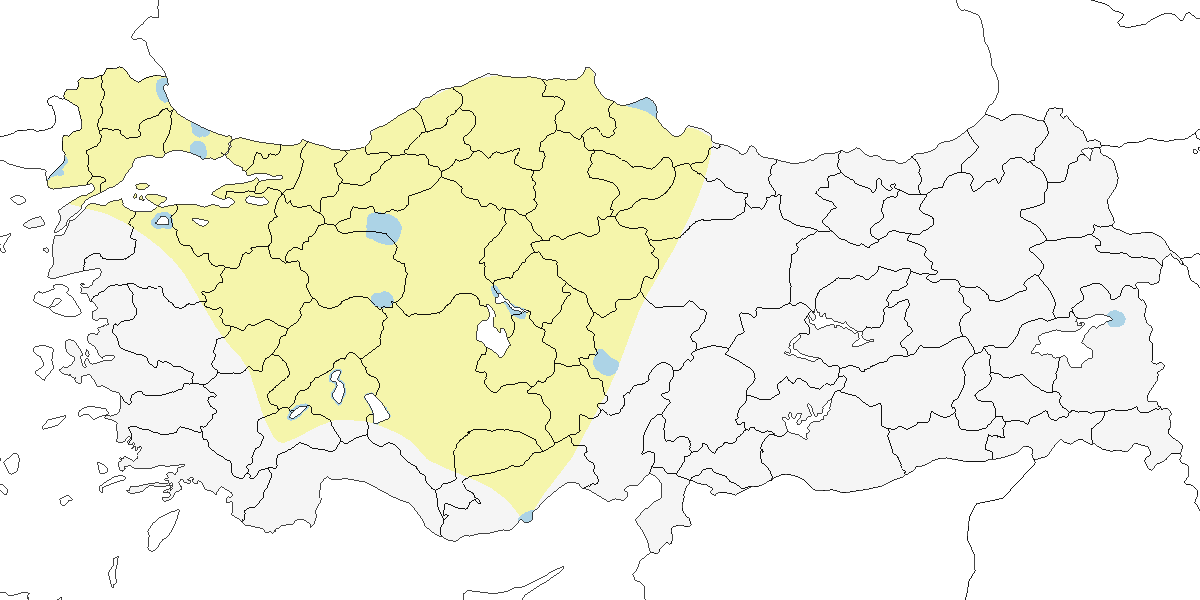
\includegraphics{images/harita_Cygnus columbianus.png}

\textbf{Üreme}

Türkiye'de yuvalamaz. Sibirya Tundra kuşağında yuvalar.

\textbf{Alttürler ve Sınıflandırma}

Türkiye'de Eski Dünya'da yaşayan \emph{bewickii} alttürü bulunur; bu
alttür, gaga kökü ve yüz derisinin sarı olmasıyla tanınır. Amerika'da
yaşayan \emph{columbianus} alttürü ise siyah gaga ve siyah yüz derisi
ile kolaylıkla ayırt edilebilir.

\section{Ötücü Kuğu}\label{uxf6tuxfccuxfc-kuux11fu}

\emph{Cygnus cygnus}, Whooper Swan

\textbf{\emph{Yaygın olarak ve az sayıda görülen bir kış konuğudur.}}

Ekim sonu ile nisan başı arasında yaygın olarak az sayıda görülen bir
kış konuğudur. Ocak ve şubat aylarında en yüksek sayıya ulaşır.
Trakya'da Meriç Deltası hem Türkiye'deki ana toplama bölgesidir, üstelik
türün Balkanlar'daki en önemli kışlama alanıdır. 25 Ocak 1998'de Meriç
Deltası'nda 1200 birey kaydedilmiş, bu Türkiye'deki en yüksek sayıdır
(Boyla and Eken, 1998). Türkiye'ye gelen kuşlar, Ukrayna ve Kırım ile
Batı Karadeniz Bölgesi arasındaki deniz üzeri göç rotasını kullanır
(Brazil, 2003). Doğuda, 30 Ekim 1995'te Sodalı Gölü'nde 164 birey
(Adızel, 1998), 1992'de Diyarbakır Kabaklı Barajı'nda 133 birey
kaydedilmiştir (DHKD, 1992).

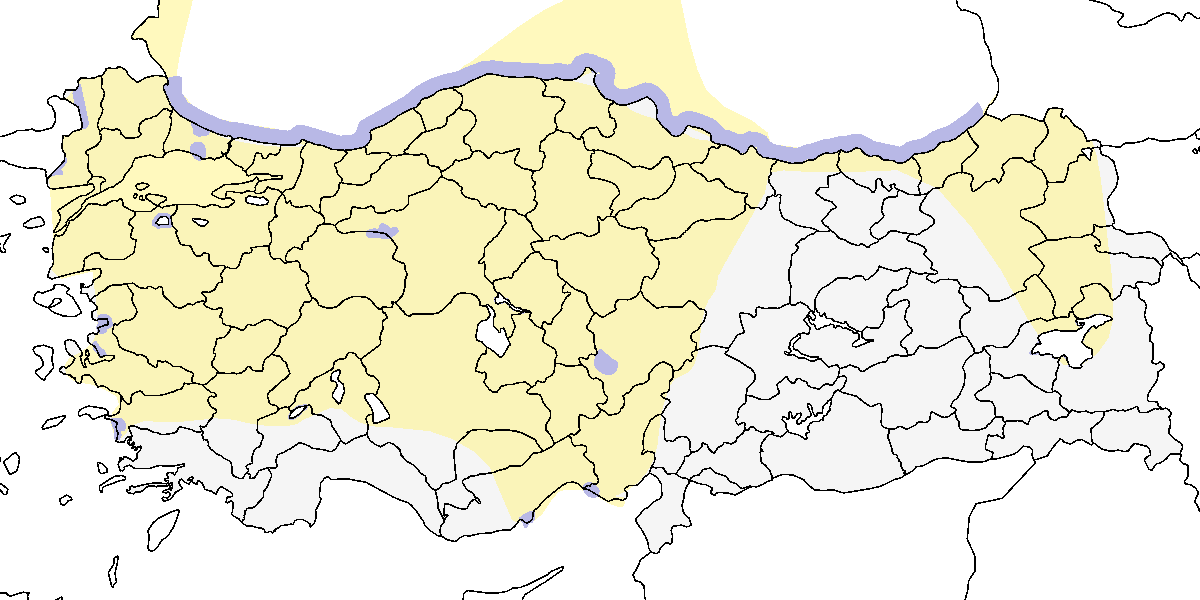
\includegraphics{images/harita_Cygnus cygnus.png}

\textbf{Üreme}

Türkiye'de yuvalamaz. Üreme bölgesi Kuzey Avrasya'dadır

\textbf{Alttürler ve Sınıflandırma}

Monotipik bir türdür.

\section{Nil Kazı}\label{nil-kazux131}

\emph{Alopochen aegyptiaca}, Egyptian Goose

\textbf{\emph{Durumu belirsizdir. Çoğunlukla egzotik tür kategorisinde
değerlendirilir.}}

28 Nisan 1986'da Kulu Gölü'nde gözlenen bireyin doğal ve rastlantısal
bir konuk olduğu düşünülmüştür. 11 Nisan 1911'de Urfa'nın güneyinde iki
birey gördüğünü söyleyen Weigold'un (1912-13) kaydı kabul edilmemiştir
(Kasparek, 1992).

İstanbul ve Ankara'da gözlenen kuşların esaretten kaçmış olabileceği
düşünülmektedir. 6-13 Temmuz 2002'de Ankara'daki bir parkta bir çift
fotoğraflanmış; 31 Mart 2012'de İstanbul Riva'da, 13 Mart 2012'de Ankara
Hacettepe Kampüsü'nde, 5-24 Kasım 2013'de Etimesgut'ta ve 25 Mayıs-13
Haziran 2014'de Eymir Gölü'nde birer birey gözlenmiştir.

1906 ve 1928 yılları arasında Kıbrıs'ta nadir görülen bir kış göçmeni
olarak kaydedilmiş ve 1958, 1962 ve 1989 yıllarında bireyler
gözlenmiştir. Eskiden Suriye ve Filistin'de ürediği düşünülmüş (Vaurie,
1965), ancak sonrasında Suriye'de hiçbir güvenilir kaydın olmadığına
karar verilmiştir (Baumgart et al., 1995; Kumerloeve, 1967a).

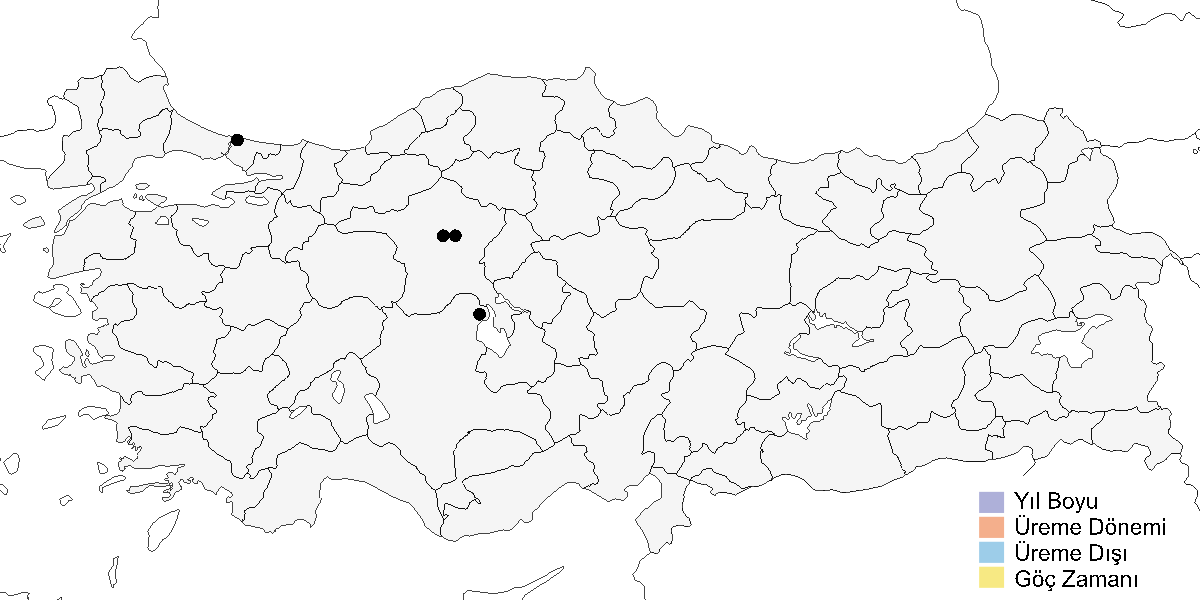
\includegraphics{images/harita_Alopochen aegyptiaca.png}

\textbf{Üreme}

Türkiye'de yuvalamaz. Üreme alanları çoğunlukla Sahra Altı Afrika'dadır.

\textbf{Alttürler ve Sınıflandırma}

Monotipik bir türdür.

\section{Suna}\label{suna}

\emph{Tadorna tadorna}, Common Shelduck

\textbf{\emph{Lokal olarak az sayıda ürer. Aynı zamanda lokal olarak çok
sayıda bulunabilen bir kış konuğudur.}}

Ege Bölgesi, Göller Bölgesi, İç ve Doğu Anadolu'da geniş ve tuzlu
sulakalanlarda ürer. Başlıca üreme alanları Gediz Deltası, Bolluk Gölü,
Kulu Gölü, Tuz Gölü ve Van Gölü çevresidir. Gediz Deltası'nda 1996
yılında üreyen popülasyonun 8 çift olduğu tahmin edilmiştir (Eken,
1997a). 24 Haziran 1992'de Bolluk Gölü'ndeki bir adada 12 yuva tespit
edilmiştir.

Üreme sonrası tüy değiştiren kuşlar, ağustos ile ekim ayları arasında
toplanır. Bu dönemde Erçek Gölü'nde 2500 birey, Kulu Gölü'nde ise 700
birey sayılmıştır.

Kışlayan toplam nüfus genellikle 1000-5000 birey arasında değişir. Ana
kışlama alanı olan Yumurtalık Lagünü'nde, 16 Şubat 2006'da 5390 birey
kaydedilmiştir. Acıgöl'de ise 1969-70 yıllarında 3450 birey, 1968-69
yıllarında 4900 birey, 2004 yılında 1802 birey ve 2005 yılında 2928
birey sayılmıştır. Diğer alanlarda daha küçük gruplar halinde kışlar.

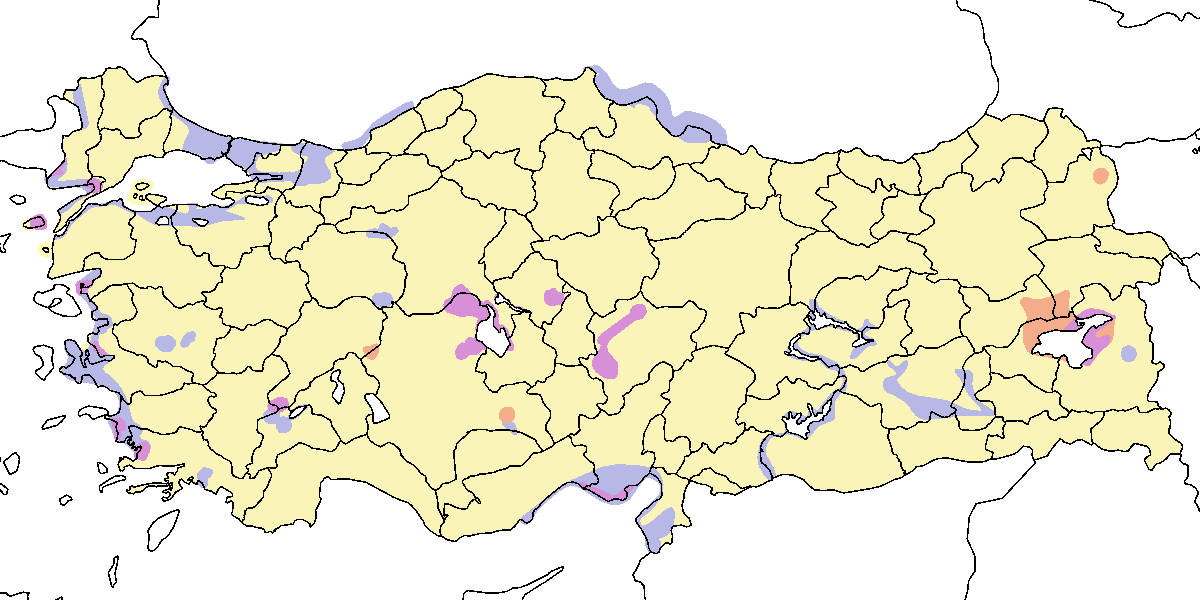
\includegraphics{images/harita_Tadorna tadorna.png}

\textbf{Üreme}

\textbf{Yuvalama Alanı:} Geniş, sığ ve tuzlu sulakalanlarda, adalar,
sedde duvarları ve çalı altlarında yuvalar.\\
\textbf{Yuvası:} Avrupa'da yuvaların çoğu tavşan oyuklarında, tünelin
1-2 metre içinde bulunur. Ancak Türkiye'deki yuvalar genellikle
yerdedir. Bolluk Gölü'ndeki yuvaların bazıları tamamen açıkta, bazıları
ise kısmen ya da tamamen çalı altında, bir tanesi ise doğal bir oyuğun
içinde bulunmuştur.\\
\textbf{Yumurta Sayısı:} Genellikle 6-9 yumurta bıraktığı gözlenmiştir.
Bolluk Gölü'ndeki yuvalarda gözlenen 10-18 yumurtanın, birden fazla dişi
tarafından bırakılmış olması muhtemeldir.\\
\textbf{Üreme Dönemi:} Gediz Deltası'nda haziran başında yavrular
gözlenmiştir (Eken, 1997a). İç Anadolu'da nisan sonu ile haziran
başında, Doğu Anadolu'da ise haziran ortasında yumurtladığı
düşünülmektedir.

\textbf{Alttürler ve Sınıflandırma}

Monotipik bir türdür.

\section{Angıt}\label{angux131t}

\emph{Tadorna ferruginea}, Ruddy Shelduck

\textbf{\emph{Yaygın ve çok sayıda bulunan yerli türdür. Kışın göç alır,
sayıları artar.}}

Üremek için genellikle yüksek kesimlerdeki küçük gölcükler, baraj
gölleri, ıslak çayırlar ve dereleri tercih eder; birçok ördek ve kaz
türünün aksine büyük sulakalanlarda yuvalamaz. İlk tahminlere göre
üreyen popülasyonun 4000 ile 8000 çift arasında olduğu öne sürülmüştür
(Tucker and Heath, 1994). Ancak, kış ortası su kuşu sayımlarına
dayanarak popülasyonun azaldığı düşünülmüş ve üreyen popülasyonun
1200-5100 çift olduğu tahmin edilmiştir (Emirogullari et al., n.d.).

Temmuz ve eylül ayları arasında tüy değişimi için bazı sulakalanlarda
büyük sürüler halinde toplanır. Erçek Gölü'nde 20.000, Sultan
Sazlığı'nda 11.000, Kulu Gölü'nde 10.000 ve Eylül 1936'da, bugün
kurutulmuş olan Emir Gölü'nde 10.000-15.000 birey sayılmıştır. Kış
öncesinde Kasım 2004'te Sarıyar Barajı'nda 8.000 birey ve Kuyucuk
Gölü'nde 6.000 birey kaydedilmiştir.

Kış aylarında daha yaygın olarak görülür. En yüksek kış sayımında
Türkiye genelinde 10.115 birey kaydedilmiş olup (Çağlayan et al., 2005),
genellikle 4000-4500 birey sayılmıştır. Ocak-Şubat 1993'te sadece 711
birey, 18 Ocak 2004'te Sarıyar Barajı'nda 5636 birey ve 18 Şubat 2006'da
7641 birey kaydedilmiştir. İç Anadolu'da üreme sonrası toplanan
sürülerde bir azalma gözlenirken, baraj göllerinin sayısında artış
olmuştur. Kış sayımı toplamlarının yaz sonu toplamlarından düşük olması,
türün dağınık şekilde kışladığını veya kış aylarında güneye göç ettiğini
göstermektedir. Toplam kışlayan nüfusun 2600 ile 28.500 birey arasında
değiştiği tahmin edilmektedir (Emirogullari et al., n.d.).

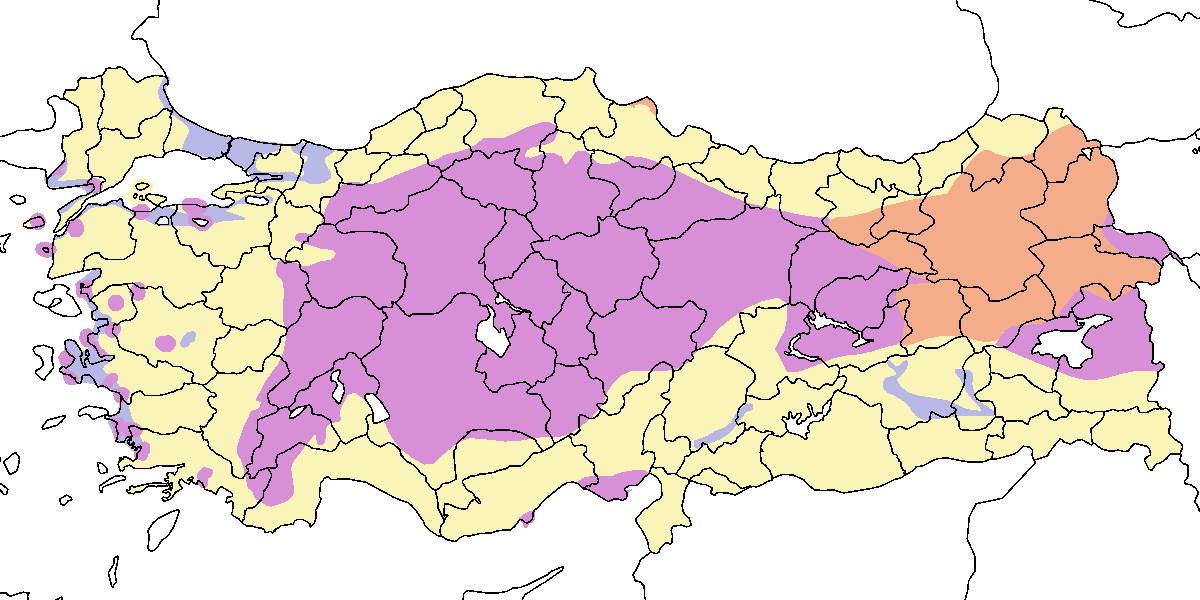
\includegraphics{images/harita_Tadorna ferruginea.png}

\textbf{Üreme}

\textbf{Yuvalama Alanı:} Genellikle göl kenarındaki sarp kayalıklarda,
tepelerde ve yamaçlardaki çukur ve çatlaklarda, açık alanlarda yuvalar.
Sıkça kayalıklarda yuva yaptığı gözlenmiştir. Beyşehir Gölü'ndeki bir
adada, kayaların ve harabelerin taşları arasında ürediği kaydedilmiştir.
22-24 Mayıs 1998'de Ereğli yakınlarındaki bir kayalıkta, muhtemelen eski
bir Kızıl Şahin yuvasında kuluçkaya yattığı gözlenmiştir.\\
\textbf{Yuvası:} Türkiye'de yuvası bitki artıkları, hav tüyleri ve bazı
diğer tüylerle kaplanmış bir oyuk şeklindedir. 30 Nisan 2003'te Akköy
yakınlarındaki dik bir yamaca giren bir dişi, muhtemelen bir tavşan
yuvası olan bir oyuğa girerken gözlenmiş, ancak oyuğun derin olması
nedeniyle yuva incelenememiştir.\\
\textbf{Yumurta Sayısı:} Genellikle 8-12 yumurta bıraktığı
kaydedilmiştir.\\
\textbf{Üreme Dönemi:} Akdeniz ve Ege bölgelerinde mart sonu yumurtlama
başlar. Diğer bölgelerde kuluçka nisan ve mayıs aylarında gerçekleşir.

\textbf{Alttürler ve Sınıflandırma}

Monotipik bir türdür.

\section{Boz Ördek}\label{boz-uxf6rdek}

\emph{Mareca strepera}, Gadwall

\textbf{Lokal olarak birkaç alanda yuvalar. Yaygın olarak nispeten az
sayılarda görülen bir kış konuğudur.}

Kızılırmak Deltası, bu türün Türkiye'deki en önemli üreme alanıdır ve
yaklaşık 200 çift burada ürer. Türkiye'de toplam üreyen popülasyonun 500
ile 5000 çift arasında olduğu düşünülmüştür (Tucker and Heath, 1994).
Ancak, günümüzde bu sayının azaldığı açıktır.

İç Anadolu'daki ilkbahar göçü marttan nisan başına kadar belirgin bir
şekilde gözlenir. Akdeniz'deki kıyısal sulakalanlarda ise nadiren
1000'den fazla birey kaydedilir. Kış ortası sayımlarda 1967'de Manyas
Gölü'nde 5000, 1969'da Akşehir Gölü'nde 7500 ve 1971'de Hotamış
Sazlığı'nda 2490 birey sayılmıştır. 1967-1973 yılları arasında ülke
genelinde çoğunlukla 3000'den fazla birey kaydedilirken, 1986-2005
yılları arasında bu sayı 1000-1500 seviyelerine düşmüştür. Son yıllarda
ise yeniden artış göstermiş ve 2020 kışında Kızılırmak Deltası'nda
10.000'den fazla birey sayılmıştır.

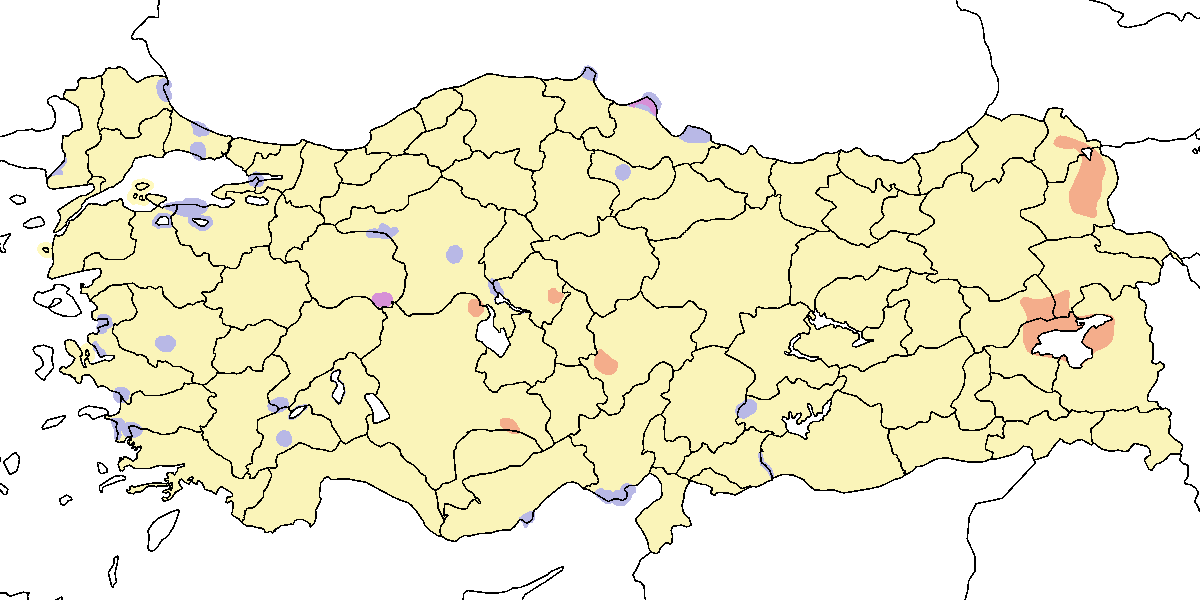
\includegraphics{images/harita_Mareca strepera.png}

\textbf{Üreme}

\textbf{Yuvalama Alanı:} Göl kıyılarında ve adalarındaki yoğun bitki
örtüsü, sazlıklar ve sık bitkilerle kaplı taşkın alanlarda yuvalar.
Kızılırmak Deltası, Karamık Gölü, Kulu Gölü, Bolluk Gölü, Mogan Gölü,
Ahlat Sazlıkları, Haçlı Gölü ve Van Gölü'nde yuvaladığı gözlenmiştir.\\
\textbf{Yuvası:} Yuva, yerde bir çukura kurulur ve bitkisel malzeme ile
dişinin tüyleriyle kaplanır.\\
\textbf{Yumurta Sayısı:} Türkiye'deki yuvalarda yumurta sayısı 6-15
arasında değişir. İç Anadolu'da 7-15 yumurtalı yuvalar gözlenmiş ve bu
yuvaların bir kısmında 1 ila 6 yumurtanın başka ördek türlerine ait
olduğu tespit edilmiştir. Kulu Gölü'ndeki yuvalarda 6 Mayıs 1972'de 3-11
yumurta ve 14 Temmuz 1971'de 7 yumurta sayılmıştır (Kasparek, 1987). 17
Mayıs 2004'te Bolluk Gölü'ndeki bir yuvada 8 yumurta bulunmuştur.\\
\textbf{Üreme Dönemi:} Kızılırmak Deltası'nda nisan başında yumurtlamaya
başlar (Hustings and Dijk, 1994). İç Anadolu'da nisan sonu ile temmuz
arasında, Doğu Anadolu'da ise haziran ile eylül arasında yavrulara
rastlanmıştır.

\textbf{Alttürler ve Sınıflandırma}

Türkiye'de nominat alttür görülür. Tür eskiden \emph{Anas} cinsi altında
sınıflandırılıyordu.

\section{Fiyu}\label{fiyu}

\emph{Mareca penelope}, Eurasian Wigeon

\textbf{\emph{Yaygın olarak çok sayıda bulunan kış konuğu ve geçit
türüdür.}}

Ege, Akdeniz ve İç Anadolu'nun sulakalanlarında kalabalık sürüler
halinde kışlar. 1960'lı ve 1970'li yıllarda düzenli olarak ortalama
150.000 birey sayılmıştır. En yüksek sayılar 1968'de 208.600, 1969'da
ise 458.800 birey olarak kaydedilmiştir. Ancak günümüze gelindiğinde
ciddi bir düşüş yaşanmış, 1986 ile 2005 yılları arasındaki düzenli
sayımlarda yalnızca dört yıl 40.000'den fazla birey kaydedilebilmiştir.
Genellikle eylül sonunda gelir ve nisan sonuna kadar kalır.

İç Anadolu'da mart sonu ve nisan başı arasında yüksek sayılarda göç
eder. Bazı göçmen bireyler mayıs sonuna kadar bölgede kalır. Nadiren de
olsa, İç ve Doğu Anadolu'da üremeden yazı geçiren bireyler gözlenebilir.

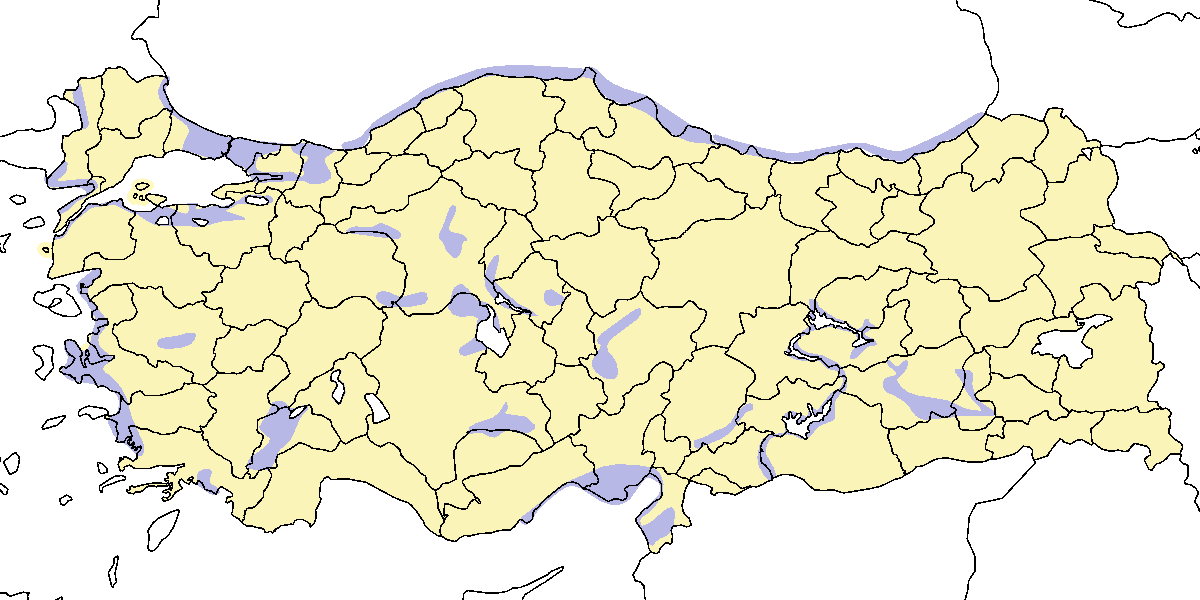
\includegraphics{images/harita_Mareca penelope.png}

\textbf{Üreme}

Türkiye'de yuvalamaz. Kuzey Avrupa'da yuvalar.

\textbf{Alttürler ve Sınıflandırma}

Monotipik bir türdür. Eskiden \emph{Anas} cinsi altında
sınıflandırılırdı.

\section{Yeşilbaş}\label{yeux15filbaux15f}

\emph{Anas platyrhynchos}, Mallard

\textbf{\emph{Yaygın olarak üreyen yerli bir türdür. Kışın göç alır,
yüksek sayılara ulaşabilir.}}

Uygun yaşam alanlarının bulunduğu bölgelerde az sayıda yuvalar. En
yaygın olarak İç Anadolu Bölgesi'ndeki sulakalanlarda görülür, diğer
bölgelerde ise oldukça lokal bir dağılım gösterir. En yüksek yuvalama
sayısı, 400-600 çiftin kaydedildiği Kızılırmak Deltası'nda olmuştur
(Hustings and Dijk, 1994).

Sonbaharda göç alır ve popülasyonu artar. Kışlayan gruplar nisan başına
kadar bölgede kalır. En yüksek sayılarda Karadeniz, Marmara ve Ege
bölgelerinde kaydedilirken, Akdeniz ve İç Anadolu'da nispeten az sayıda,
Güneydoğu Anadolu ve Doğu Anadolu'da ise çok daha az sayıda bulunur.
2000 ve 2020 yılları arasında kışlayan nüfus ortalama 20.000 birey
civarındayken, kışın sert geçtiği 2005 yılında Türkiye genelinde toplam
106.140 birey ve Kızılırmak Deltası'nda 50.000 birey sayılmıştır.

1960'lı ve 1970'li yıllarda kışlayan popülasyonun 100.000'ler
seviyesinde olduğu bildirilmiştir. 1967 yılında Kızılırmak ve Yeşilırmak
Deltası'nda yaklaşık 52.000, Büyük Menderes Deltası'nda 42.000; 1968
yılında Manyas ve Uluabat Gölleri'nde 42.000; 1969 yılında Büyük
Menderes Deltası'nda 80.000, Akyatan Lagünü'nde 40.000 ve Amik Gölü'nde
30.000; 1970 yılında ise Meriç Deltası'nda 34.500 ve Sultansazlığı'nda
30.000 birey kaydedilmiştir.

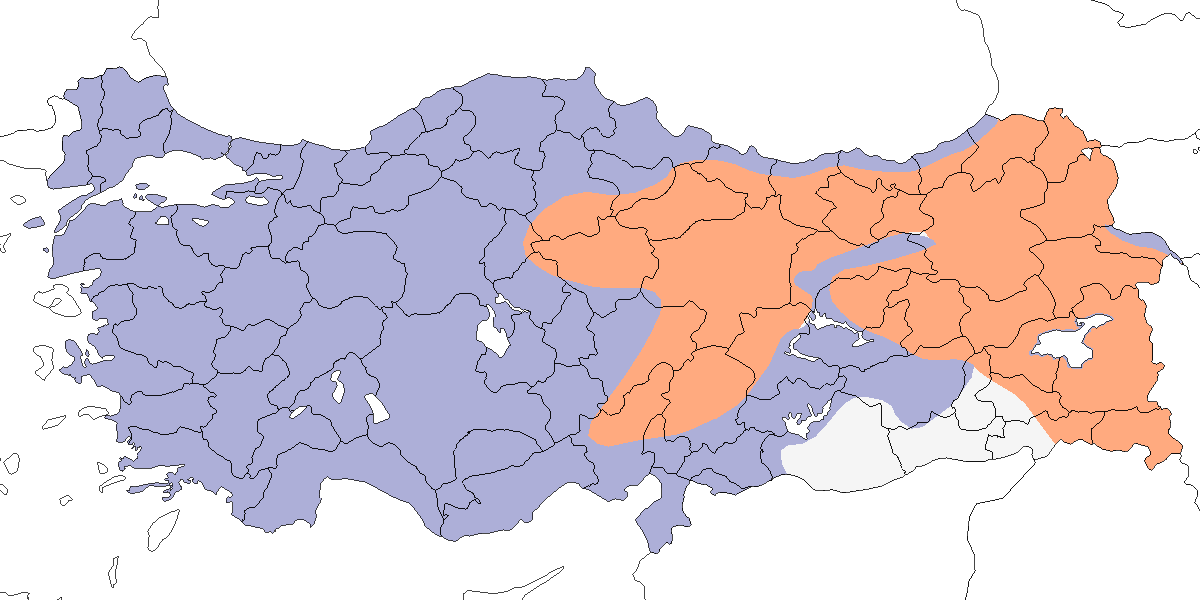
\includegraphics{images/harita_Anas platyrhynchos.png}

\textbf{Üreme}

\textbf{Yuvalama Alanı:} Göl ve nehir adalarında, sazlıklarda veya göl,
sazlık ve subasar çayırların kıyılarındaki sık bitki örtüsü içinde
yuvalar.\\
\textbf{Yuvası:} Yuvasını genellikle bitki örtüsünün altına, topraktaki
bir oyuğa yapar. Diğer bölgelerde ağaç kovuklarına veya karga gibi
kuşların ağaçlardaki eski yuvalarına yuvaladığı bilinir; ancak
Türkiye'de bu tür yuvalara henüz rastlanmamıştır.\\
\textbf{Yumurta Sayısı:} Genellikle 5-9 yumurta bırakır, ancak yumurta
sayısı 2-14 arasında değişebilir. Bir yuvadaki yumurtaların 14'ten fazla
olması, birden fazla dişinin aynı yuvaya yumurtladığını gösterir.\\
\textbf{Üreme Dönemi:} Kıyı bölgelerinde marttan itibaren, diğer
bölgelerde ise nisan veya mayısta yumurtlar. Yavrular mayıs başından
temmuz sonuna kadar görülebilir. \textbf{Marmara:} 18 Nisan 1993'te
Kocaçay Deltası'nda yavrularıyla gözlenen bir dişi, en erken üreme
kaydıdır (Ertan, 1996). \textbf{Karadeniz:} 19-20 Mayıs 1992'de Yeniçağa
Gölü'nde yuvalarda hem yumurta hem yavrular gözlenmiştir. 5 Mayıs
1992'de Kızılırmak Deltası'nda sezonun ilk yavruları görülmüştür
(Hustings and Dijk, 1994). 16 Mayıs 1967'de Manyas Gölü'nde dokuz
yumurtalı bir yuva kaydedilmiştir. 20 Haziran 1973'te Trakya'da altı
yavrulu bir dişi gözlenmiştir. \textbf{İç Anadolu:} 1971'de Yarma'daki
birçok yuvada diğer türlerin yumurtalarına rastlanmıştır; örneğin, bir
yuvada 17 Yeşilbaş, üç Boz Ördek ve üç Macar Ördeği yumurtası
tanınmıştır. 13-15 Temmuz 1971'de Kulu Gölü'nde sekiz yuva incelenmiş ve
yuvalarda 2-12 yumurta bulunmuştur (Kasparek, 1987). Başka bir tarihte,
mayıs ve haziran aylarında yumurtalı yuvalar ve mayıs ortasından
itibaren yavrular gözlenmiştir. \textbf{Doğu Anadolu:} En erken kayıt,
14 Haziran 1968'de Erçek Gölü'nde kaydedilen yavrulardır. Aynı yerde 28
Haziran 1968'de beş ve sekiz yumurtalı iki yuva bulunmuş, 9 Haziran
2001'de Balık Gölü'nde iki yumurtalı yuva kaydedilmiştir (Kasparek and
Ven, 1983).

\textbf{Alttürler ve Sınıflandırma}

Türkiye'de nominat alttürü bulunur.

\section{Kaşıkgaga}\label{kaux15fux131kgaga}

\emph{Spatula clypeata}, Northern Shoveler

\textbf{\emph{Lokal olarak az sayıda yuvalar. Aynı zamanda yaygın olarak
çok sayıda bulunan bir geçit türü ve kış konuğudur.}}

İç Anadolu ve Doğu Anadolu'daki birkaç büyük sulakalan ile Kızılırmak
Deltası'nda yuvalar (Boyla et al., 2018). 1970'lerde Kulu Gölü ve
Kızılırmak Deltası bilinen üreme alanlarıdır.

Tüm bölgelerde yaygın olarak kaydedilen bir geçit türüdür. Göçmen
gruplar, ilkbaharda mart başından nisan sonuna kadar, sonbaharda ise
eylül ortasından kasım başına kadar zaman zaman yüksek sayılarda
görülür. Eylül ayında Kulu Gölü'nde 7000, Sultansazlığı'nda 9000 ve mart
sonunda Kızılırmak Deltası'nda 4500 birey sayılmıştır.

Ülkenin batı ve orta bölgelerinde kışlar. 2000 ile 2020 yılları arasında
ülke çapında kışlayan kuş sayısı genellikle 5000 bireyin altında
kalmıştır; ancak kışın soğuk geçtiği 2005 yılında 13.576 birey
sayılmıştır. 1990'lı yıllarda daha yüksek sayılar kaydedilirdi; örneğin,
1993'te toplam 7898 birey, 1999'da ise 13.114 birey kaydedilmiştir. Daha
önceki yıllarda yapılan sayımlarda; 1967'de Büyük Menderes Deltası'nda
23.000, Kızılırmak Deltası'nda 8000 birey ve 1993'te 4564 birey
sayılmıştır. 1967-1973 yılları arasında İç Anadolu'daki alanlarda
3000'den fazla bireyden oluşan sürüler olağandı.

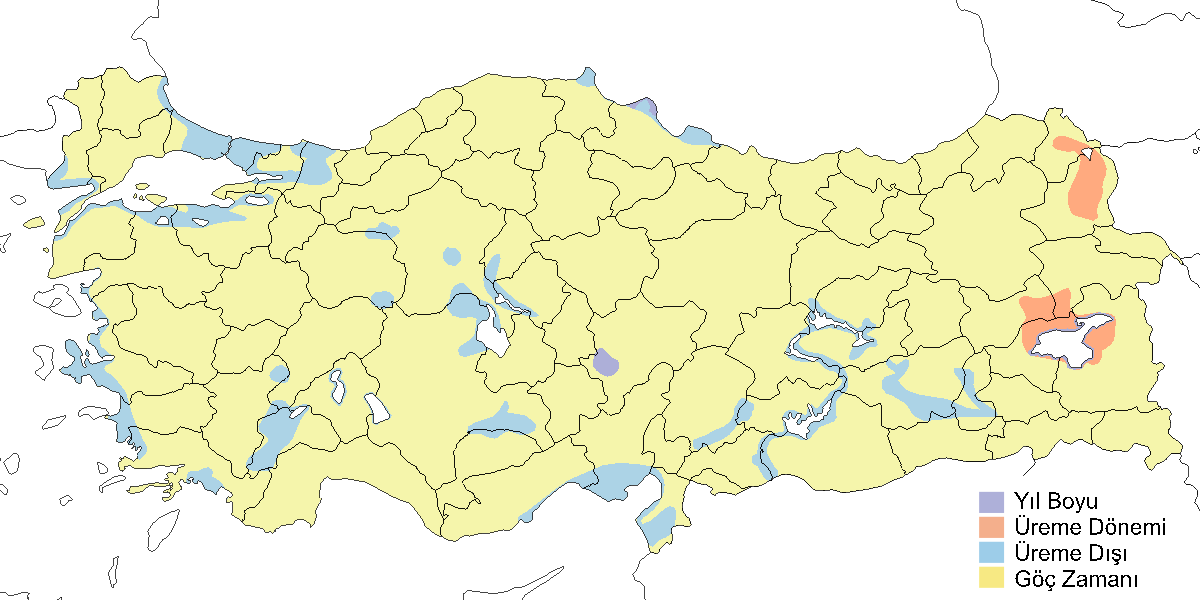
\includegraphics{images/harita_Spatula clypeata.png}

\textbf{Üreme}

\textbf{Yuvalama alanı}: Büyük sulakalanlarda yuvalar.\\
\textbf{Yuvası}: Kulu Gölü'nde bir adadaki seyrek bitki örtüsü içinde
yuvalamıştır. Yuvasını çıplak zeminde sığ bir oyuk açarak yapar ve içine
ot, bitki gövdeleri ve tüylerini karıştırarak döşer.\\
\textbf{Yumurta sayısı}: 8-10 yumurta bıraktığı kaydedilmiştir.\\
\textbf{Üreme Dönemi:} Türkiye'deki üreme sezonu hakkında yeterli veri
bulunmamaktadır; diğer ülkelerde ise üreme sezonu genellikle nisan başı
ile mayıs sonu arasındadır.\\
\textbf{Karadeniz:} 6-7 Temmuz 1972'de Kızılırmak Deltası'nda dört ve
beş yavrulu iki dişi kaydedilmiştir (Dijksen and Kasparek, 1985). 1992
yılında üreme kanıtlanamamış ve popülasyonun 0-1 çift olduğu
belirtilmiştir (Hustings and Dijk, 1994). 1971 yılı Temmuz ortasında
kaydedilen yumurtalı yuvalar, başarısız bir üremenin ardından
gerçekleşen ikinci bir üreme denemesi olarak değerlendirilmiştir.\\
\textbf{İç Anadolu:} 14-15 Temmuz 1971'de Kulu Gölü'ndeki bir adada
sekiz ve on yumurtalı iki yuva tespit edilmiştir. 5-6 Ağustos 1972'de
iki ve dört yavrulu iki yavru grubu gözlenmiştir (Kasparek, 1987). 31
Mayıs 1987'de Kulu Gölü'nde yavrular gözlenmiş, 19 Haziran 1992'de dokuz
yumurtalı bir yuva bulunmuştur. Haziran 1977'de Eşmekaya'da beş
yavrusuyla birlikte bir dişi gözlenmiştir (Schubert, 1979).\\
\textbf{Doğu Anadolu:} 29 Mayıs 1969'da Van Gölü'nde kur davranışı
gözlenmiştir.

\textbf{Alttürler ve Sınıflandırma}

Monotipik bir türdür.

\section{Kılkuyruk}\label{kux131lkuyruk}

\emph{Anas acuta}, Northern Pintail

\textbf{Nispeten yaygın olarak bulunan bir geçit türü ve kış konuğudur.
Nadiren yuvalar.}

Son yıllarda 1998 ve 1999'da, tek bir alanda, Girdev Gölü'nde üremiştir.
İlkbaharda ve yazın İç Anadolu'da birçok erişkin kaydı olsa da,
kanıtlanmış üreme kayıtları az sayıdadır. Üreyen popülasyonun 500 ile
1000 çift olması iddiası tamamen geçersizdir (Tucker and Heath, 1994).

Genellikle eylül ortasından nisan başına kadar batı ve orta bölgelerde
görülür.

Ülke genelinde kışlayan nüfus 10.000 bireyden azdır. 1986'da toplam
25.700 birey, 1992'de 11.070 birey ve 1999'da 13.573 birey kışlamıştır.
Kışlama popülasyonunda çarpıcı bir azalma belgelenmiştir. 60'li yıllarda
düzenli olarak 100.000'in üzerinde sayılırdı. Örneğin, 1967'de Büyük
Menderes Deltası'nda 60.000 birey, Emir Gölü'nde 70.000 birey, 1969'da
Akyatan Gölü'nde 100.000 birey ve Gâvur Gölü'nde 50.000 birey
kaydedilmiştir. Bilhassa ılıman geçen kışlarda daha yüksek sayılarda
kaydedilebilir. Eski tarihlerde bazı alanlardaki sayımların sonuçlarının
güvenilirliği sorgulanabilir, örneğin, 1970'de Sultansazlığı'ndaki
sayılan 160.000 birey muhtemelen abartılı bir tahmindir. Bu ve diğer
ördek türlerinin önemli sayılarda kışladığı birkaç sulakalan kısmen ya
da tamamen kurutulmuş durumdadır. Diğer yandan son yıllarda oluşan baraj
göllerinde kışlamaya başlamıştır.

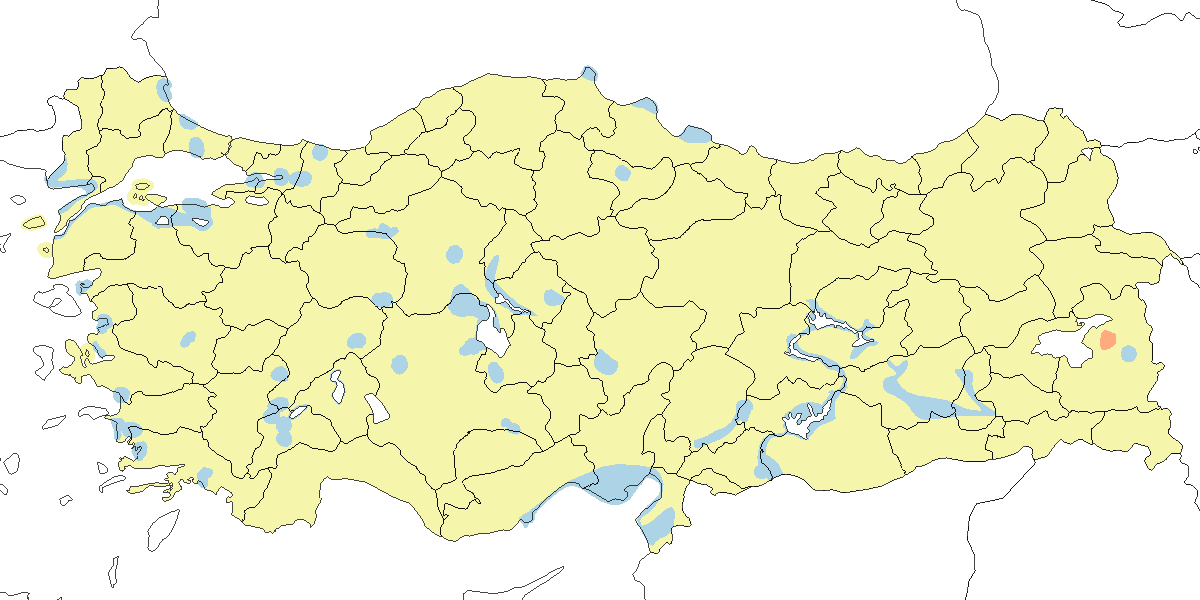
\includegraphics{images/harita_Anas acuta.png}

\textbf{Üreme}

\textbf{Yuvalama alanı}: Büyük göllerde ve sulakalanlarda yuvalar.\\
\textbf{Yuvası}: Kulu Gölü'ndeki büyük adada kıyı vejetasyonu içinde
yuvalamıştır. Yerdeki bir delikte yaptığı yuvasını bitkisel malzemeler,
hav tüyleri ve kontür tüyleri ile kaplanmıştır.\\
\textbf{Yumurta sayısı}: 6-10 yumurta koyduğu kaydedilmiştir.\\
\textbf{Üreme dönemi}: Görünüşe göre mayıs ayında yumurtlar.
\textbf{KAR.} Kızılırmak Deltası'nda üreme davranışları gözlenmiş,
ürediği kesinleşmemiştir (Hustings and Dijk, 1994). \textbf{AKD.}
Haziran 1998 ve 1999'da Girdev Gölü'nde yavrular gözlenmiştir.
\textbf{İÇA.} 22 Mayıs 1992'de Kulu Gölü'nde yedi ve on yumurtalı iki
yuva, 19 Haziran 1992'de 6 ila 9 yumurtalı beş yuva bulunmuştur. 24
Haziran 1992'de Bolluk Gölü'ndeki bir çalının altına gizlenen yuvada 11
yumurta sayılmıştır.

\textbf{Alttürler ve Sınıflandırma}

Türkiye'de nominat alttürü bulunur.

\section{Çıkrıkçın}\label{uxe7ux131krux131kuxe7ux131n}

\emph{Spatula querquedula}, Garganey

\textbf{Yaygın olarak az sayıda üreyen bir yaz göçmenidir. Bunun yanında
göç döneminde daha yaygın ve çok sayıdadır. Nadiren kışlar.}

Ördeklerin arasında esasen yaz göçmen olan tek türdür. Şubat ortasından
itibaren görülmeye başlar, ekim sonuna kadar kalır. Leylekle beraber en
erken gelen göçmen kuşlardandır. Sazlık sulakalanları tercih eder, en
yoğun ürediği alanlar İç ve Doğu Anadolu'dadır. Güneydoğu Anadolu'da iki
alanda üremesi olasıdır.

İlkbahar ve sonbahar boyunca Türkiye'nin tüm bölgelerinde yüzlerce,
hatta binlerce birey sürüler halinde gözlenebilir. İlkbahar geçişi şubat
sonundan mayıs sonuna kadar devam eder. Sonbahar geçişinde ise ağustos
sonu ile eylül başı arasında Karadeniz kıyıları boyunca göçmen sürülere
rastlanabilir.

Nadiren Marmara, Ege ve Akdeniz'de az sayıda kışlar. Olağandışı yumuşak
geçen 1968-69 kışında Göksu Deltası'nda 3000 birey ve Gâvur Gölü'nde
5000 birey sayılmıştır. Güncel tarihlerde; Ocak 2002'de Güllük
Deltası'nda 65 birey, Şubat 2002'de Bafa Gölü'nde 58 birey, Aralık
2002'de Çukurova'da 89 birey, 4 Aralık 2010'de Karkamış Barajı'nda iki
birey kışlamıştır.

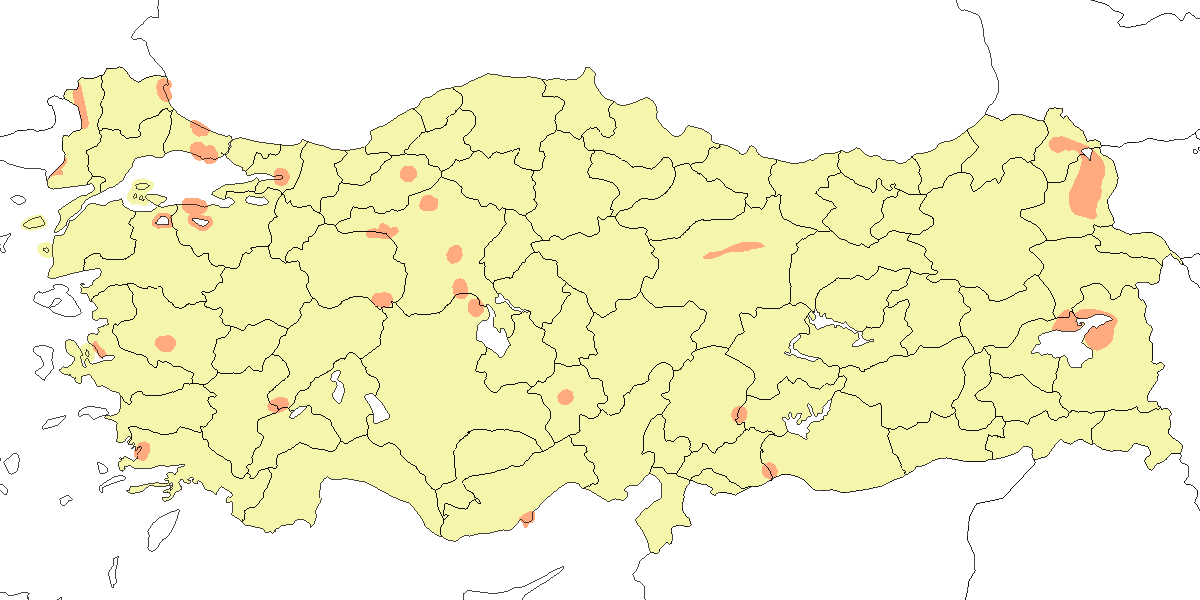
\includegraphics{images/harita_Spatula querquedula.png}

\textbf{Üreme}

\textbf{Yuvalama alanı}: Sazlık sulakalanlarda yuvalar.\\
\textbf{Yuvası}: Göl kenarlarındaki ıslak çayırlar, bataklıklar ve
sazlıklarda, ikisinin bir arada olduğu alanlarda ve göl kenarındaki
vejetasyonun içinde ürer.\\
\textbf{Yumurta sayısı}: Türkiye'den veri yoktur, diğer yerlerde olağan
yumurta sayısı 8-11'dir.\\
\textbf{Üreme dönemi}: Nisan ortasından itibaren ürer. Yavrular temmuza
kadar görülebilir. \textbf{KAR.} 19 Mayıs 1992'de Yeniçağa Gölü'nde yeni
bozulmuş ancak yumurtaların taze olduğu açıkça anlaşılan iki yuva, 6
Mayıs 1993'te yakınlardaki ıslak bir çayırlıkta bir yuva bulunmuştur. 13
Mayıs 1986'da Abant Gölü'nde 17 yavru ve bir dişi gözlenmiş, yumurtlama
tarihinin nisan ortası civarında olduğunu hesaplanmıştır. 2 Ağustos
1971'de Kızılırmak Deltası'nda bir çift ve yedi yavru kaydedilmiştir.
\textbf{İÇA.} 10-15 Mayıs 1991'de Hotamış Sazlığı'nda yavrulu birkaç
çift gözlenmiş (Kirwan, 1993), 27 Temmuz 1971'de Kulu Gölü'nde büyük
yavruları olan altı çift kaydedilmiş, Haziran ve Temmuz 1968'de Mogan
Gölü'nde 1-2 kuluçka gözlenmiş, 27 Temmuz 1971'de Yarma'da büyük
yavruları olan en az dört çift tespit edilmiştir.

\textbf{Alttürler ve Sınıflandırma}

Monotipik bir türdür.

\section{Çamurcun}\label{uxe7amurcun}

\emph{Anas crecca}, Eurasian Teal

\textbf{\emph{Lokal olarak az sayıda ürer. Bunun yanında yaygın olarak
ve çok sayıda bulunan kış konuğudur.}}

İç Anadolu, Doğu Anadolu ve Kızılırmak Deltası'nda yuvalar. Kızılırmak
Deltası'nda 1992'de 15-20 çift üremiştir (Hustings and Dijk, 1994), Doğu
Anadolu'dan teyit edilmiş üreme kaydı ise çok azdır.

Geçiş sırasında eylül başından nisan başına kadar ülkenin batı ve orta
bölgelerinde yaygın olarak çok sayıda görülebilir. Marmara ve Karadeniz
bölgelerinde ara sıra yüksek sayılarda kaydedilebilir.

Kışın hem iç bölgelerde hem de kıyısal sulakalanlarda yüksek sayıda
bulunur. Ülke çapında kışlayan nüfus 100.000 birey seviyesindedir. Son
yıllarda kışlayan nüfusta düşüşler yaşanmış, örneğin 1988'de 21.000
birey ve 1989'da 13.400 birey sayılmıştır. Bu düşüş, aslında diğer yüzey
ördeklerinde olduğu gibi 1960'lardan beri süre gelmektedir. 1968-69'da
toplam 270.400 birey ve 1969-70'de 326.700 birey sayılmıştır. Son
sayımda sadece Sultansazlığı'nda 200.000 birey gözlenmiştir. Alanda
sayılan ancak türü tespit edilemeyen 400.000 ördeğin de çamurcun
olabileceği düşünülürse, alandaki kışlayan çamurcun sayısı 600.000 birey
olabilir.

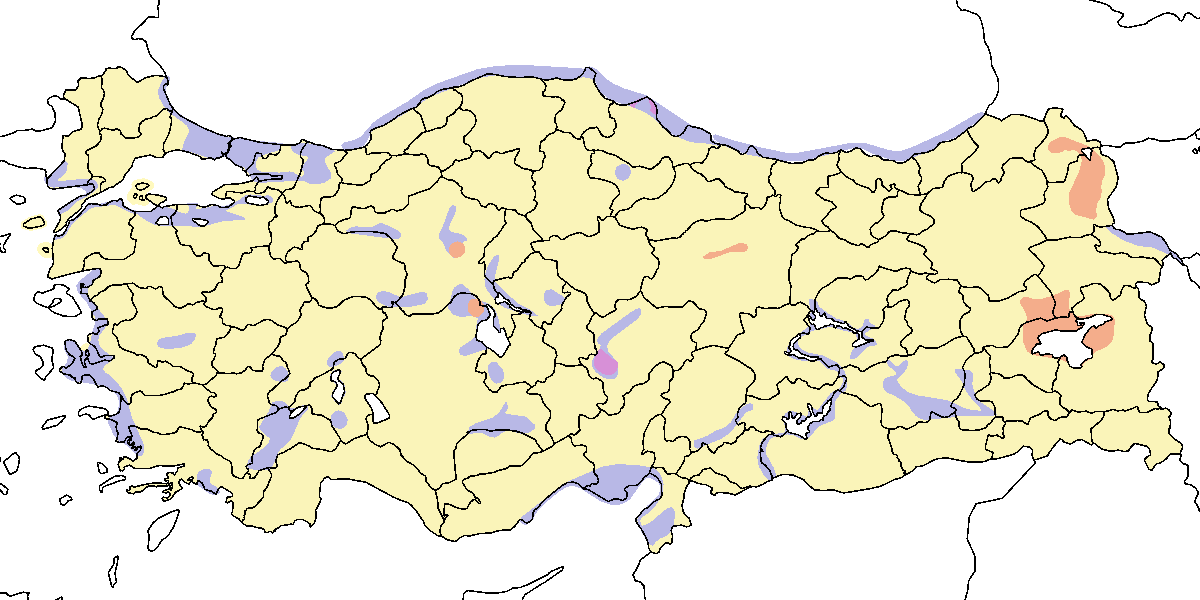
\includegraphics{images/harita_Anas crecca.png}

\textbf{Üreme}

\textbf{Yuvalama alanı}: Göllerde ve sazlıklarda ürer.\\
\textbf{Yuvası}: Yuva ve yumurta sayısı Türkiye'den bilinmez. Diğer
yerlerde yuvasını yerdeki bir oyuğa yapar ve genellikle yapraklar,
bitkisel malzemeler, hav tüyleri ve kontur tüyleriyle kaplar.
Sulakalanlarda yüksek otların üzerine yuvalar, nadiren sudan uzağa da
yuva yapabilir.\\
\textbf{Yumurta sayısı}: Türkiye'den veri yoktur, ancak diğer yerlerde
olağan yumurta sayısı 8-12'dir.\\
\textbf{Üreme dönemi}: Nisan ortasından itibaren ürer, yavrular temmuza
kadar görülebilir. \textbf{KAR:} 29 Mayıs 1979'da Kızılırmak Deltası'nda
içinde yumurta olan bir yuva bulunmuş, 28 Temmuz 1971'de dokuz yavrulu
bir dişi ve 6 Ağustos 1971'de beş yavrulu bir dişi gözlenmiştir (Dijksen
and Kasparek, 1985). 1992'de popülasyonun 15-20 çift olduğu belirlenmiş,
5 Mayıs'ta dikkati başka yere çekme davranışı gözlenmiş ancak hiçbir
yuva bulunamamıştır (Hustings and Dijk, 1994). \textbf{İÇA}: 14 Mayıs
1991'de Hotamış Sazlığı'nda yavrularıyla birlikte birkaç erişkin
gözlenmiş, bu da yumurtaların en geç nisan ortasında koyulmuş olduğunu
göstermiştir (Kirwan, 1993). 5-6 Ağustos 1972'de Kulu Gölü'nde iki
dişinin 7 ve 10 yavrusu gözlenmiştir (Kasparek, 1987). \textbf{DOA}: 24
Haziran 1983'te Haçlı Gölü'nde tek yavrulu bir dişi kaydedilmiştir.

\textbf{Alttürler ve Sınıflandırma}

Türkiye'de nominat alttürü bulunur.

\section{Yaz Ördeği}\label{yaz-uxf6rdeux11fi}

\emph{Marmaronetta angustirostris}, Marbled Duck

\textbf{\emph{Türkiye'de üreyen nüfus yok olmuştur.}}

Göksu Deltası'nda üreyen popülasyonun 2013 yılından sonra yok olmasıyla,
üreyen tür olarak Türkiye'deki soyunun tükendiği söylenebilir. Tek tük
Doğu Akdeniz, Güneydoğu ve Doğu Anadolu'da görülebilir. Marmara, Ege ve
Karadeniz bölgelerinde eski tarihli kayıtları vardır. En yakın üreme
alanı Irak'taki Mezopotamya Bataklıkları'dır.

Mart başından ekim başına kadar kaydedilen bir yaz konuğu idi. Göksu
Deltası'ndaki üreyen popülasyon, 1989 ile 2013 arasında adım adım
azalmıştır. 1989 ve 1991'de yaklaşık 50 çift tespit edilmiş, 2000'li
yıllarda bu sayı 10 çifte düşmüş, 2010 ile 2013 arasında sadece 1 ila 2
çift kalmış ve 2014 yılından itibaren alanda görülmemeye başlamıştır. Bu
nedenle Türkiye'de üreyen nüfusunun yok olduğu kabul edilmiş (Boyla et
al., 2018) ve Yaz Ördeği, Yılanboyun'dan sonra Türkiye'de soyu tükendiği
belgelenen ilk kuş türü olmuştur.

1987 yılında Çukurova'da, bugün yok edilmiş olan Dipsiz Gölü'nde 32 çift
tespit edilmiştir. İç Anadolu'da Ereğli Sazlığı'nda muhtemelen 1-4 çift,
Hotamış Sazlığı'nda 10-15 çift ve Sultansazlığı'nda 1-4 çift üremiştir.
Van Gölü havzasında ise Erciş Gölü ve Van Sazlığı'nda az sayıda ürediği
teyit edilmiş, bunun yanında Ağrı çevresi, Ahlat Sazlıkları, Bendimahi
Deltası ve Kuyucuk Gölü'nde üreme döneminde görülmüştür. 1987 yılında
ülke nüfusunun 50-100 çift olduğu düşünülmüştür. Üreme sonrasında
Çukurova ve Göksu Deltası'nda 100-200 bireyin toplandığı bilinir.
Nadiren az sayıda kışlamıştır. En son sayımlarda 1993'te Çukurova'da
dört, 1997'de aynı alanda 35 birey sayılmıştır.

Amik Gölü'nün kurutulmasından önce muhtemelen önemli sayılarda
bulunuyordu (Kumerloeve, 1963). Konya havzasındaki Yarma Sazlıkları,
Gönenç Gölü ve Karapınar Ovası'nda (Grimmett and Jones, 1989) muhtemelen
üremiştir. Mogan Gölü ve Eber Gölü gibi diğer birkaç alanda da üremiş
olabilir. Bu alanlar ekolojik özelliklerini kaybettikleri ve türe uygun
üreme habitatları barındırmadıkları için artık üremeye elverişli
değildir. Üreme sonrası toplanan bireyler, o yıllarda toplam ülke nüfusu
hakkında fikir verebilir. Ağustos 1967'de Çukurova'da 2000 birey ve
Göksu Deltası'nda 450 birey sayılmıştır.

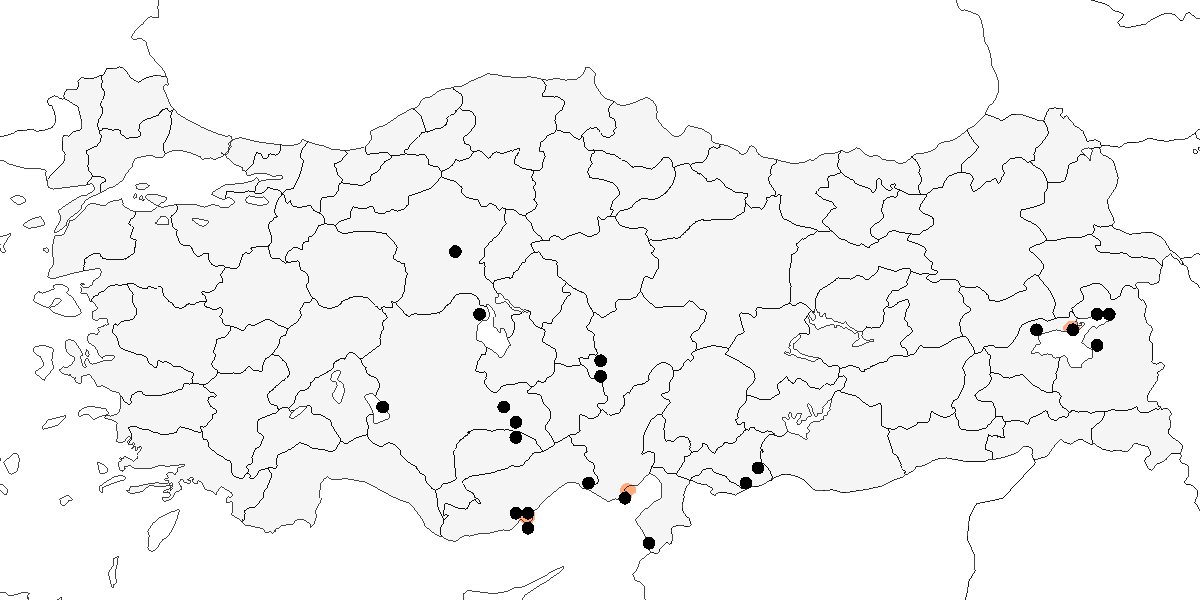
\includegraphics{images/harita_Marmaronetta angustirostris.png}

\textbf{Üreme}

\textbf{Yuvalama Alanı:} Çukurova ve Göksu Deltası'nda sığ ve ötrofik
göllerde bulunmuştur. Genellikle sazlık adaların, bitişik havuzlar ve
sazlıkların bulunduğu yoğun sualtı vejetasyonuna sahip sığ göllerin
çevresinde ürer ve geniş sulakalanları tercih eder. Sanılanın aksine acı
veya tuzlu sularda değil tatlı suları tercih eder.\\
\textbf{Yuvası:} 9 Haziran 1993'te Göksu'da, kofanın (\emph{Juncus})
baskın olduğu ve yakınlarda sazların (\emph{Phragmites}) da bulunduğu
bataklık bir bölgede sığ gölcüklerin olduğu bir alanda, yaklaşık 1 m
çapındaki bir \emph{Juncus} kümesinin içinde, sudan yaklaşık 0,7 m
yüksekte gizlenmiş iki yumurtalı bir yuva bulunmuştur. Yuva sazlardan ve
bitki gövdelerinden yapılmış dayanıklı bir kâse şeklindedir ve ince
bitkisel malzemeyle kaplanmıştır; hav tüyü kullanılmamıştır.\\
\textbf{Yumurta Sayısı:} Yumurta sayısı 2 ile 12 arasında değişir,
ortalama 6,5 yumurta olarak hesaplanmıştır (Green, 1993). Diğer
bölgelerde ise tipik yumurta sayısı 9-13'tür (5-18).\\
\textbf{Üreme Dönemi:} 22 Mayıs 1971'de Çukurova'da kaydedilen altı
yavru, en erken kayıttır ve yumurtlamanın nisanın ikinci yarısında
başladığını gösterir. Ana yumurtlama dönemi, mayısın ikinci yarısıyla
haziran başı arasındadır. Yavrular en erken 7 Haziran'da ortaya çıkar ve
temmuz sonuna kadar küçük yavrular görülebilir. Tamamen palazlanmış
yavrular temmuz başında kaydedilmiştir. \textbf{AKD:} 1991'de Göksu
Deltası'nda yaklaşık 50 çiftten en az 31'i yavru çıkarmıştır. Aynı yıl
Göksu Deltası'nda 11 yuvada 8-13, 5 yuvada 4-6 ve bir yuvada 15 yavru
sayılmıştır. 15 yavrunun, iki dişinin yumurtalarının bir araya
gelmesiyle oluştuğu düşünülmektedir. Benzer şekilde 15-18 Temmuz 1992'de
bir dişi 32 yavruyla görülmüştür (Green, 1993). 10 Temmuz 1967'de hem
büyük hem küçük yavrular haziran ve temmuzda az sayıda gözlenmiştir
(Vielliard, 1968). \textbf{İÇA:} 4-5 Haziran 1971'de Yarma Sazlığı'nda 6
ve 13 yumurtalı iki yuva bulunmuş, bir yuvada bir Yeşilbaş yumurtası
görülmüştür. 12 Haziran 1998'de Kulu Gölü'nde tek yavrulu bir erişkin
kaydedilmiş ve temmuz ayında üç farklı alanda yavrular gözlenmiştir.
\textbf{DOA:} 22 Temmuz 1987'de Van Sazlığı'nda küçük yavruları olan iki
çift gözlenmiş, bu gözleme dayanarak yumurtlamanın haziran ortasında
olduğu tahmin edilmiştir. Aynı alanda temmuz sonunda ve ağustos başında
genç bireyler kaydedilmiştir.

\textbf{Alttürler ve Sınıflandırma}

Monotipik bir türdür.

\section{Macar Ördeği}\label{macar-uxf6rdeux11fi}

\emph{Netta rufina}, Red-crested Pochard

\textbf{\emph{Lokal olarak nispeten çok sayıda ürer. Kışın daha
yaygındır ve bazı alanlarda yüksek sayılarda toplanır.}}

İç Anadolu'daki geniş sodalı ya da tatlı sazlık sulakalanlarda çok
sayıda ürer. Sultansazlığı'nda yüksek sayılarda bulunur. 1990'larda
Ereğli Sazlığı'nda 500 çift üremişken 1998'de sadece 20 çift üremiş,
alanın kurutulmasıyla buradan tamamen yok olmuştur. Kızılırmak
Deltası'nda 1992'de 50-75 çift üremiştir (Hustings and Dijk, 1994).
Diğer alanlarda nispeten yüksek sayılarda yuvalayanlar yerli veya yarı
göçmendir. Çukurova sulakalanları ve Göksu Deltası'nda üreyen nüfus
1990'dan sonra azalmıştır. Türkiye'de üreyen popülasyon 1000-5000 çift
olarak tahmin edilmiştir (Tucker and Heath, 1994). Son yıllarda İç
Anadolu'da üreyen kuşların sayılarında yaşanan azalma, güncel ulusal
nüfusun çok daha az olduğuna işaret etmektedir.

Ülke genelinde geçiş sırasında doğu bölgeleri dışında daha yaygındır.
Çoğu zaman yüzeyi donmaya daha az eğilimli olan baraj göllerini tercih
eder. Ocak 1967'de 12.000 birey sayılmış, bunun 7000'i bugün kurutulmuş
olan Amik Gölü'ndendir. Türkiye genelinde 1992'de 5249, 1996'da 6522 ve
1999'da 6228 birey sayılmıştır. 2000'li yıllarda toplam sayıda artış
görülmüş, sadece Beyşehir Gölü'nde Şubat 2003'te 10.000 birey ve Ocak
2005'te 20.000 birey sayılmış, son sayımda hem toplam hem de alan rekoru
kırılmıştır.

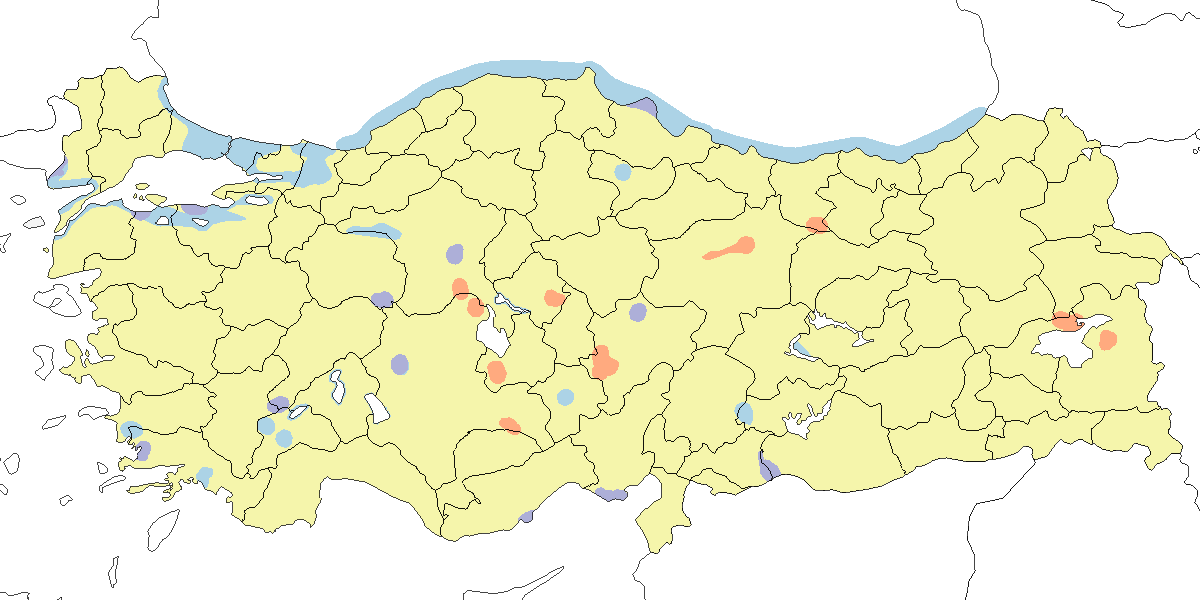
\includegraphics{images/harita_Netta rufina.png}

\textbf{Üreme}

\textbf{Yuvalama Alanı:} Yoğun sazlıkların ve su kenarı bitkilerinin
bulunduğu tatlı ya da sodalı göllerde ve su aynalarına sahip sazlıklarda
ürer.

\textbf{Yuvası:} Yerdeki bir oyuğa yaptığı yuvasını bitkisel malzeme,
hav tüyleri ve tüylerle kaplar. Çoğunlukla yoğun vejetasyonun içine,
nadiren açıkta (örneğin adalarda) ya da nemli alanlarda su seviyesinin
üzerindeki saz öbeklerinin ya da diğer sucul bitkilerin içine genellikle
iyice gizlenmiş bir yuva yapar.

\textbf{Yumurta Sayısı:} Türkiye'de gözlenen yumurta sayısı 4-12 olup,
ortalama 8,3'tür (18 yuvada). Bir yuvada bulunan 24 yumurta muhtemelen
birden fazla dişiye aittir. Yavru sayısı 2-12 arasında değişir ve 16
yuvada ortalama 6,2'dir. Sadece 2-4 yavru çıkarabilmiş 6 dişi ortalamayı
düşürmüştür.

\textbf{Üreme Dönemi:} Nisan sonu ile temmuz başı arasında yumurtlar.
Yavrular temmuz sonuna kadar görülebilir. \textbf{MAR:} 1 Mayıs 1993'te
Kocaçay Deltası'nda yumurtalı bir yuva bulunmuştur (Ertan, 1996).
\textbf{KAR:} Kızılırmak Deltası'nda 27 Mayıs 1992'de beş yumurtalı bir
yuva bulunmuş, 4 Haziran 1992'de yaklaşık bir haftalık ilk tüylü yavru
kaydedilmiş (Hustings and Dijk, 1994) ve 27 Mayıs 1979'da sekiz yavrulu
bir aile gözlenmiştir (Dijksen and Kasparek, 1985). \textbf{AKD:} 18
Temmuz 1992'de Karamık Gölü'nde küçük yavrulardan oluşan bir aile
gözlenmiştir. \textbf{İÇA:} Çoğu mayısta olmak üzere 25 Nisan'da yumurta
kayıtları vardır. En geç kayıt 19 Haziran 1992'de 12 yumurtalı bir
yuvadır. Biri 11 Mayıs'ta, çoğu haziranda olan birçok yavru kaydı
vardır, en geç 8 Temmuz 1967'de (Vielliard, 1968) ve 5 Ağustos 1972'de
küçük yavrular gözlenmiştir. \textbf{DOA:} 21-22 Temmuz 1986'da Van
Gölü'nde 7-8 yavrulu üç yavrulu bir aile kaydedilmiştir.

\textbf{Alttürler ve Sınıflandırma}

Monotipik bir türdür.

\section{Elmabaş Patka}\label{elmabaux15f-patka}

\emph{Aythya ferina}, Common Pochard

\textbf{Nispeten yaygın ve çok sayıda bulunan yerli ve yarı göçmen,
yaygın ve çok sayıda bulunan kış konuğudur.}

İç ve Doğu Anadolu'daki sulakalanlarda orta sayılarda üreyen yerli ve
yarı göçmendir. 1992'de Kızılırmak Deltası'nda 300-350 çiftin ürediği
tahmin edilmiştir (Hustings and Dijk, 1994). Uygun habitatların azlığı
nedeniyle Karadeniz, Güneydoğu Anadolu ve diğer bölgelerde lokal olarak
bulunur. Muhtemelen gerçek üreme durumunu çarpıtacak şekilde, hatırı
sayılır sayıda üremeyen birey özellikle İç ve Doğu Anadolu'da yazı
geçirir.

Kışın ve geçiş dönemlerinde ülke genelinde yaygın ve boldur. Son
yıllarda ortalama 67.000 bireyden fazla sayılmaktadır. 1996 yılında
Beyşehir Gölü'nde 47.000, Uluabat Gölü'nde 42.000 ve ülke genelinde
toplamda 250.000 birey sayılmıştır, bu en yüksek kayıtlardandır. 1999'da
Eğirdir Gölü'nde 40.000, ülke genelinde ise 137.000 kuş sayılmıştır. 18
yıllık Kış Ortası Su kuşu sayımlarının ortalaması 93.000 kuştur. İstisna
olarak 1968-69 kışında 355.000 bireyin kışladığı tahmin edilmiştir. Ekim
ortasından itibaren yüksek sayılar gözlemlenir; Göksu Deltası'nda Ekim
1978'de 40.000, Ekim 2002'de Sodalıgöl'de 100-130.000, Kulu Gölü'nde
Kasım 1970'de 45.000 ve Kasım 1971'de 28.000 birey kaydedilmiştir.

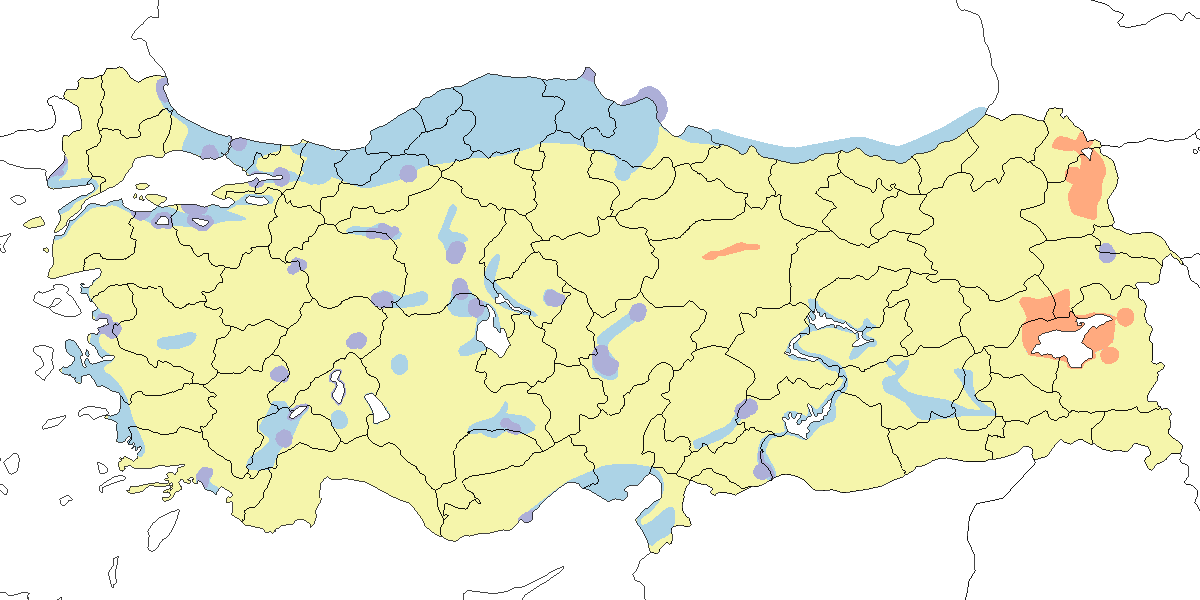
\includegraphics{images/harita_Aythya ferina.png}

\textbf{Üreme}

\textbf{Yuvalama alanı}: Göl kıyılarındaki sazlıklarda ve su aynalarının
bulunduğu sazlık bataklıklarda ürer.\\
\textbf{Yuvası:} 19 Haziran 1984'te Erçek Gölü yakınlarındaki küçük bir
gölde, sık bir örtü içindeki sazların dibine tutturulmuş ve sakarmeke
yuvasına benzer şekilde sudan yükseğe yapılmış bir yuva bulunmuştur.
Yuva, ölü saz gövdeleri ve diğer bitkisel malzemelerle derin ve düzgün
bir kâse şeklinde örülmüş, bol miktarda hav tüyü ve diğer tüylerle
kaplanmış dayanıklı bir yapıya sahiptir. Diğer bölgelerdeki yuvalar da
genellikle benzer alanlarda olup nadiren su kıyısındaki yoğun bitki
örtüsünün içinde kuru zeminde de bulunabilir.\\
\textbf{Yumurta Sayısı:} Türkiye'de yumurta sayısı kaydedilmemiştir,
ancak gözlenen yavru sayısından 8-11 yumurta bırakabileceği
düşünülmektedir. Diğer bölgelerde genellikle 6-9 yumurta bırakır.
Gözlenen yavru sayısı ortalama 6,6'dır.\\
\textbf{Üreme Dönemi:} Nisan başı ile haziran ortasına kadar yumurta
bırakır. Yavrular temmuz ayında gözlenebilir. \textbf{KAR}. Kızılırmak
Deltası'nda 11 Mayıs 1992'de hav tüyleriyle kaplı birkaç günlük yavru,
en erken kayıt olarak görülmüş ve bu da yumurtlamanın nisanın ilk
haftasında olduğunu göstermiştir (Hustings and Dijk, 1994). 14 Haziran
1984'te yaklaşık 5 günlük yavrulardan oluşan bir kuluçka ile yaklaşık üç
haftalık yavrulardan oluşan iki kuluçka gözlenmiştir (Dijksen and
Kasparek, 1985). \textbf{İÇA}. Haziran başlarında iki yumurtalı
(tamamlanmamış) bir yuva bulunmuş, Haziran 1971'de Boz Ördek yuvalarına
iki, dört ve beş yumurta bırakıldığı tespit edilmiştir. 13 Mayıs 1991'de
Hotamış'ta yumurtalı bir yuva bulunmuştur (Kirwan, 1993). 1970 yılının
mayıs ayı sonunda Eşmekaya'da küçük yavrulardan oluşan beş yavru, 1
Haziran 1969'da Sultansazlığı'nda altı yavru ve haziran-temmuz aylarında
diğer alanlarda yavrular gözlenmiştir. \textbf{DOA}. 19 Haziran 1983'te
Van Sazlığı'nda yavrularıyla birlikte sekiz dişi kaydedilmiştir.

\textbf{Alttürler ve Sınıflandırma}

Monotipik bir türdür.

\section{Pasbaş Patka}\label{pasbaux15f-patka}

\emph{Aythya nyroca}, Ferruginous Duck

\textbf{Lokal olarak az sayıda üreyen yaz konuğu, yaygın ve nispeten çok
sayıda bulunan geçit türü, yaygın ancak az sayıda kış konuğudur.}

Tüm bölgelerdeki sulakalanlarda oldukça lokal bir yaz konuğudur. En
yüksek sayılarda İç ve Doğu Anadolu bölgelerinde bulunur. Kızılırmak
Deltası (1992'de tahminen 150-200 çift (Hustings and Dijk, 1994),
Kocaçay Deltası (1993'te tahminen 70 çift (Ertan, 1996), Uluabat Gölü
(1988'de tahminen 32 çift (Welch and Welch, 1998b) ve Göksu Deltası
(yaklaşık 30 çift) önemli sayılarda ürediği alanlardır. Son yıllarda
gerçekleştirilen çalışmalarda Güneydoğu Anadolu'da üç yeni üreme alanı
belirlenmiştir. Yaz göçmenleri mart ortasından eylül sonuna kadar
gözlenir.

Türkiye popülasyonu muhtemelen dünyadaki en önemlilerinden biridir ve
1000 ile 3000 çift arasında olduğu düşünülmüş (Tucker and Heath, 1994),
sonra bu tahmin 500-600 çift olarak güncellenmiştir (Kirwan, 1997a).
Avrupa'da yayılış alanının bir kısmında yaşanan sert düşüş dikkate
alındığında, Türkiye popülasyonunun izlenmesine acil ihtiyaç
duyulmaktadır. 1990'ların sonlarında İç Anadolu'daki birkaç alanda da
azalma görülmüştür.

Geçiş sırasında az ve orta sayılarda bulunur ve ülke genelinde biraz
daha yaygındır. Az sayıda kışlar, 1992 yılında 105 birey, diğer yıllarda
50 bireyden az sayılmıştır. 1990'ların ortalarından itibaren kış
kayıtlarında bir artış gözlenmiş, bu durum muhtemelen gözlemci sayısının
artmasına bağlanmıştır. Eskiden batı ve orta bölgelerde daha çok sayıda
kışlamış, 1968-74 yıllarında 50 ile 450 birey arasında kaydedilmiştir.
Marmara Gölü'nde kaydedilen 860 birey en yüksek kayıttır. Doğu ve
Güneydoğu Anadolu'da 2005 yılında sayılan 44 birey bahsedilmeye
değerdir.

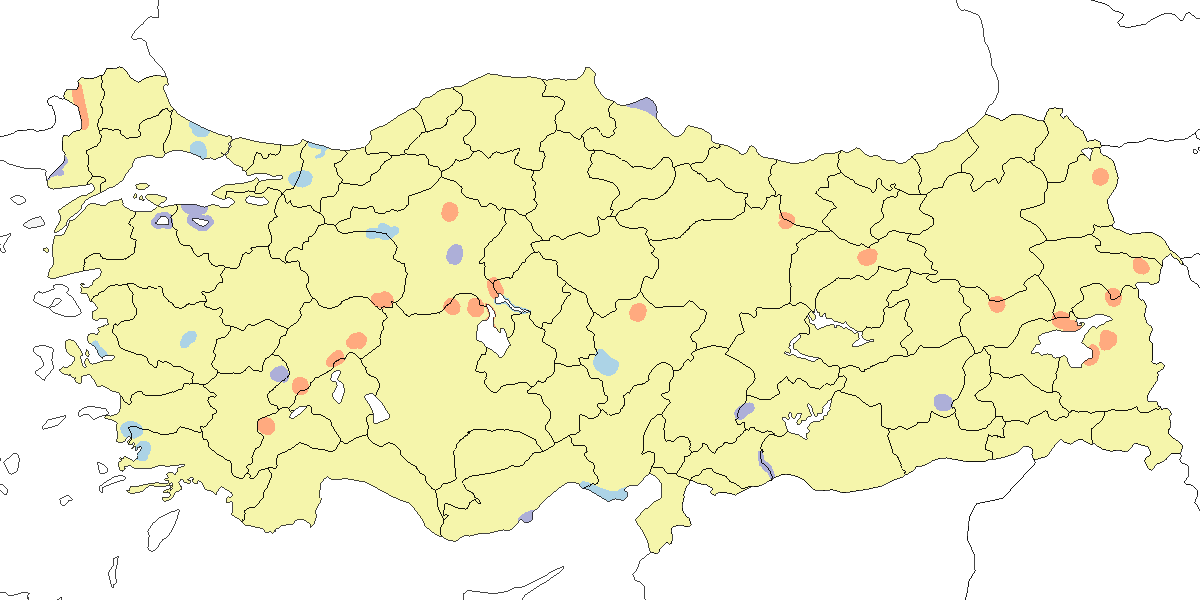
\includegraphics{images/harita_Aythya nyroca.png}

\textbf{Üreme}

\textbf{Yuvalama Alanı:} Çevresinde sazlıkların, yoğun su üstü
vejetasyonunun ve çoğunlukla daha geniş sazlıkların ve bataklıkların
bulunduğu tatlı su göllerinde ürer.\\
\textbf{Yuvası:} Su kenarındaki yoğun vejetasyonun içine yuva yapar.
Kulu Gölü'ndeki bir adada, alçak çalıların arasında çıplak zeminde hafif
bir çukurun içine yapılan yuvanın ot ve hav tüyleriyle kaplandığı
gözlenmiştir (Pforr and Limbrunner, 1982); A. Limbrunner, kişisel
görüşme).\\
\textbf{Yumurta Sayısı:} Türkiye'de gözlenen yumurta sayısı 6-8
arasındadır.\\
\textbf{Üreme Dönemi:} Nisan ile haziran başı arasında yumurta bırakır.
Yavrular ağustos ayına kadar gözlenebilir. \textbf{MAR.} 19 Haziran
1999'da Uluabat Gölü'nde bazıları küçük yavrulardan oluşan birkaç yavru
grubu gözlenmiş, 1966'da Manyas Gölü'nde de yavrular kaydedilmiştir.
\textbf{KAR.} Kızılırmak Deltası'nda çiftlerin çoğu sazlık alanlarda
gözlenmiştir. 5 Mayıs 1992'de altı yumurtalı bir yuva bulunmuş ve 1
Haziran 1992'de yumurtlamanın nisan sonlarından daha geç olmadığını
gösteren üç ve dört yavrulu iki grup kaydedilmiştir (Hustings and Dijk,
1994). 6 Ağustos 1971'de yedi yavrulu bir grup gözlenmiştir.
\textbf{AKD.} 15 Mayıs 1962'de Çukurova'da sekiz yumurtalı bir yuva
(Kirwan, 1997a), 8 Mayıs 1953'te Amik Gölü'nde yumurtalı bir yuva
(Kirwan, 1997a), ve 27 Mayıs 1933'te yumurta kanalında yumurta bulunan
bir dişi vurulmuştur (Meinertzhagen, 1935). Göksu Deltası'nda en erken
17 Haziran'da olmak üzere yedi yuva alanında yavrular gözlenmiştir.
\textbf{İÇA.} 28 Nisan 1982'de Sultansazlığı'nda yumurtalı bir yuva
bulunmuştur (Kirwan, 1997a). Mayıs 1973'te Kulu Gölü'nde altı yumurtalı
bir yuva bulunmuştur. En erken 20 Haziran'da Eber Gölü'nde olmak üzere
Çöl Gölü, Gönenç Gölü, Sultansazlığı, Mogan Gölü ve Kulu Gölü'nde
yavrular gözlenmiştir. \textbf{DOA.} Yumurtlamanın mayıs sonunda
olduğunu gösteren gözlemler 1985 ve 1987 yıllarında haziran sonunda Van
Gölü'nde ve 29 Haziran 1987'de Edremit Sazlığı'nda yapılmıştır (Kirwan,
1997a).

\textbf{Alttürler ve Sınıflandırma}

Monotipik bir türdür.

\section{Tepeli Patka}\label{tepeli-patka}

\emph{Aythya fuligula}, Tufted Duck

\textbf{\emph{Lokal ve az sayıda üreyen yaz konuğu, nispeten yaygın ve
çok sayıda bulunan kış konuğudur.}}

Çok nadir ve lokal olarak üremiştir. Kızılırmak Deltası'nda ve 1967 ile
1981'de Çalı Gölü'nde (Kars) ürediği kanıtlanmış, son alanda 20 çiftlik
bir popülasyon tespit edilmiştir. Başka bölgelerde düzenli olarak yazı
geçirir. Uluabat Gölü ve Uyuz Gölü gibi bazı alanlardaki uygun
habitatlarda çiftler gözlenmiştir. Üreme sonrasında, Temmuz 1982'de Kulu
Gölü'nde tüy değişimi için toplandıkları düşünülen 700 birey (Kasparek,
1987), Eylül 1967'de ise Sodalı Gölü'nde çoğu erkek olan 1200 birey
sayılmıştır.

Ülkenin batı ve orta bölgelerinde eylül başından nisan başına kadar
kaydedilen yaygın ve bol bulunan bir geçiş türü ve kış konuğudur.
Karadeniz'de denizde kışlar. Kış ortası sayımlarında; 1968-69 kışında
20.800 birey, 1996'da en yüksek sayı olan 58.271 birey, 1992'de yaklaşık
13.000 birey, 1993'te 16.965 birey (sadece Eğirdir Gölü'nde 10.478
birey) ve 1999'da 18.512 birey kaydedilmiştir. Son yıllarda ise ülke
toplamı genellikle 5000-10.000 birey arasındadır. En önemli kışlama
alanları Sapanca Gölü ve Eğirdir Gölü'dür.

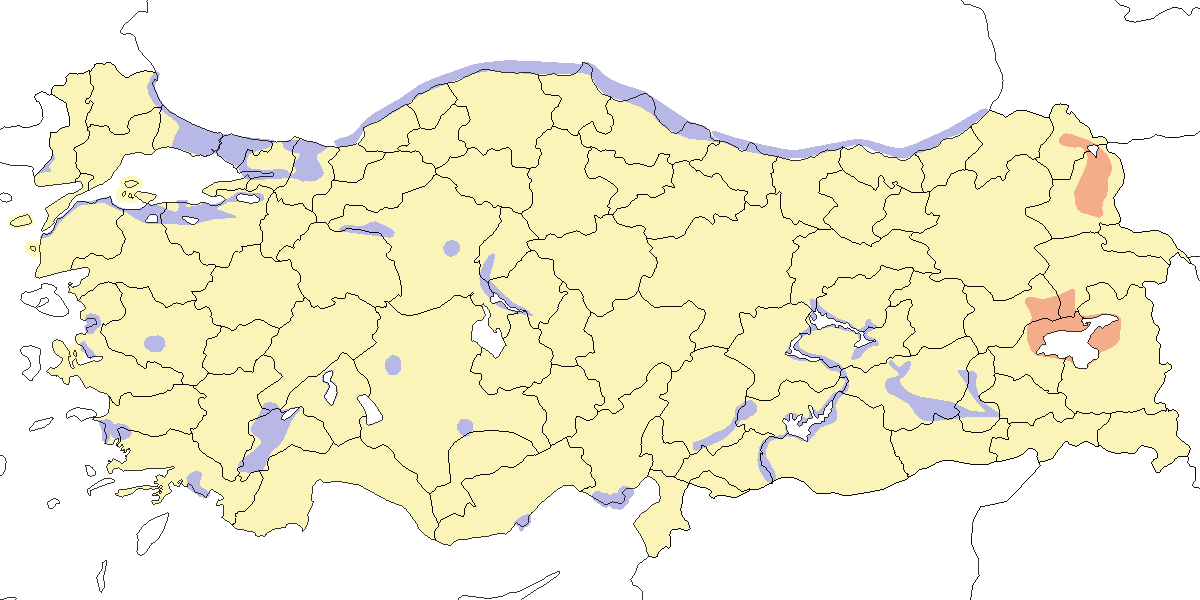
\includegraphics{images/harita_Aythya fuligula.png}

\textbf{Üreme}

\textbf{Yuvalama alanı}: Su üstü vejetasyonu olan tatlı su göllerinde
ürer.\\
\textbf{Yuvası}: Yuvasını bir bitki öbeğinin altına kurar.\\
\textbf{Yumurta sayısı}: Türkiye'de 8 yumurtalı bir yuva bulunmuştur.\\
\textbf{Üreme dönemi}: Mayıs ayında yumurta koyar, temmuz sonuna kadar
yavrular görülebilir. \textbf{KAR.} Kızılırmak Deltası'nda, 5 Mayıs
1992'de sazlıkta bir \emph{Juncus acutus} öbeğinin dibinde sekiz
yumurtalı bir yuva bulunmuş (Hustings and Dijk, 1994) ve 28 Mayıs
1968'de de ürediği kanıtlanmıştır (Dijksen and Kasparek, 1985).
\textbf{DOA.} Çalı Gölü'nde 19 Temmuz 1992'de yavrularıyla birlikte iki
dişi gözlenmiştir (Magnin and Yarar, 1997).

\textbf{Alttürler ve Sınıflandırma}

Monotipik bir türdür.

\section{Karabaş Patka}\label{karabaux15f-patka}

\emph{Aythya marila}, Greater Scaup

\textbf{\emph{Özellikle Karadeniz kıyılarında az sayıda ve düzenli
olarak görülen kış konuğudur.}}

Karadeniz ve Marmara Bölgesi'nde hemen hemen her yıl az sayıda
görülmektedir. Modern kuş tayininin başlaması sonrasında gelen kayıtlar
şöyledir (OST, 1978, 1975, 1972, 1969): Ocak-Şubat 1969'da Sakarya
Deltası'nda yedi birey, Manyas ya da Uluabat Gölü'nde dört birey
görülmüştür. Kızılırmak Deltası'ndaki Liman Gölü'nde 1990'ların
başlarında kışlayan 38 birey, 1970'lerde aynı alandan bildirilen şüpheli
kayıtların (Dijksen and Kasparek, 1985) geçerli olabileceğini
düşündürür.

Çoğu İstanbul civarından olan geçmiş veriler şöyledir: Şubat 1893'te
Çekmece'de daha çok dişi ve gençlerden oluşan bir grup gözlenmiş ve şu
anda Sofya Doğa Tarihi Müzesi'nde bulunan erkek örnek toplanmıştır
(Alléon, 1880). İstanbul Robert Kolej'de bulunan dişi örnek
(Mathey-Dupraz, 1920--24), 1998'deki bir ziyarette bulunamamıştır
(Kirwan, 1997b). 1946-47 ve 1947-48 kışlarında Çatalağzı açıklarında
(Zonguldak) belirsiz sayıda gözlenmiş (Ogilvie, 1954), 15 Ocak 1950'de
bilinmeyen bir yerden altı örnek alınmıştır (Kumerloeve, 1970a).
Büyükçekmece'de Ocak 1963'te bir erkek ve Şubat 1964'te bir dişi
kaydedilmiştir (Kumerloeve, 1970a).

Türün ilk yaz kaydı 30 Mayıs 1992'de Sodalı Gölü'nde kaydedilen iki
erkektir (Kirwan and Martins, 1994). Öte yandan, 19 Nisan 1981'de Kulu
Gölü'nde gözlenen iki birey, 12 Nisan 1990'da Göksu Deltası'nda gözlenen
yaklaşık 20 birey (Kirwan and Martins, 2000) olağandışı geç kayıtlardır.

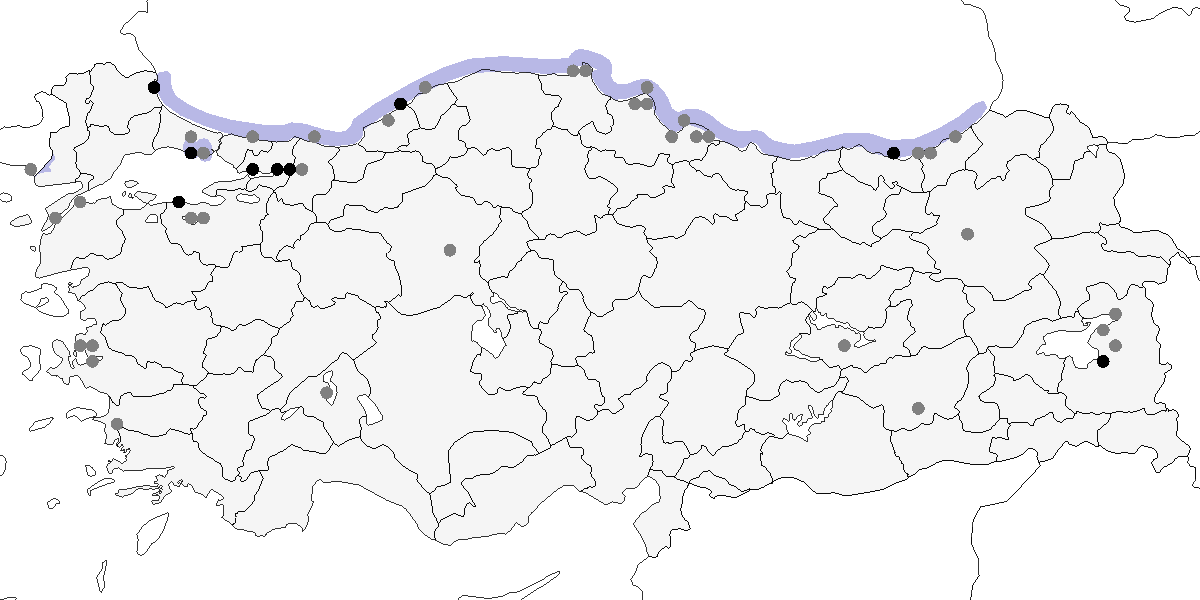
\includegraphics{images/harita_Aythya marila.png}

\textbf{Üreme}

Türkiye'de yuvalamaz. Avrasya ve Kuzey Amerika'nın kuzeyinde yuvalar.

\textbf{Alttürler ve Sınıflandırma}

Türkiye'de nominat alttürü bulunur.

\section{Pufla}\label{pufla}

\emph{Somateria mollissima}, Common Eider

\textbf{\emph{Karadeniz kıyılarında nadiren az sayıda görülür.}}

İlk üç kayıt şu şekildedir: 20 Eylül 1983'te Çernek Gölü'nde (Kızılırmak
Deltası) bir erkek (Dijksen and Kasparek, 1985), 3 Ocak 1984'te Göksu
Deltası'nda ölü bir dişi (Kasparek, 1990), 1 Şubat 1997'de Sakarya Nehri
deltasının batısında, Kefken açıklarında iyi tanımlanmış ilk kışında bir
erkek ve iki dişi (Welch and Welch, 1998a) bulunmuştur. Bundan sonra
Riva, Terkos Gölü kıyıları, İğneada, Kızılırmak Deltası, İzmit Körfezi
ve Sakarya Karasu'da 20'den fazla kayıtta 1-3 birey tespit edilmiştir.

Türkiye'de üremez, en yakın üreme kolonisi Ukrayna kıyılarındadır.
Güvenilir kayıtların tümü, 1975 yılında Ukrayna'nın Karadeniz kıyısında
bir üreme alanının keşfedilmesinden sonra olmuştur. Bu popülasyon
1990'ların ortasına kadar 1000 çifte ulaşmış ve günümüze kadar artmaya
devam etmektedir.

Şubat 1929'un ilk yarısında Tarabya ile Beykoz arasında (İstanbul
Boğazı) gözlenen bir erişkin erkek (Kumerloeve, 1970a), tanım olmadığı
için burada kabul edilmemiştir.

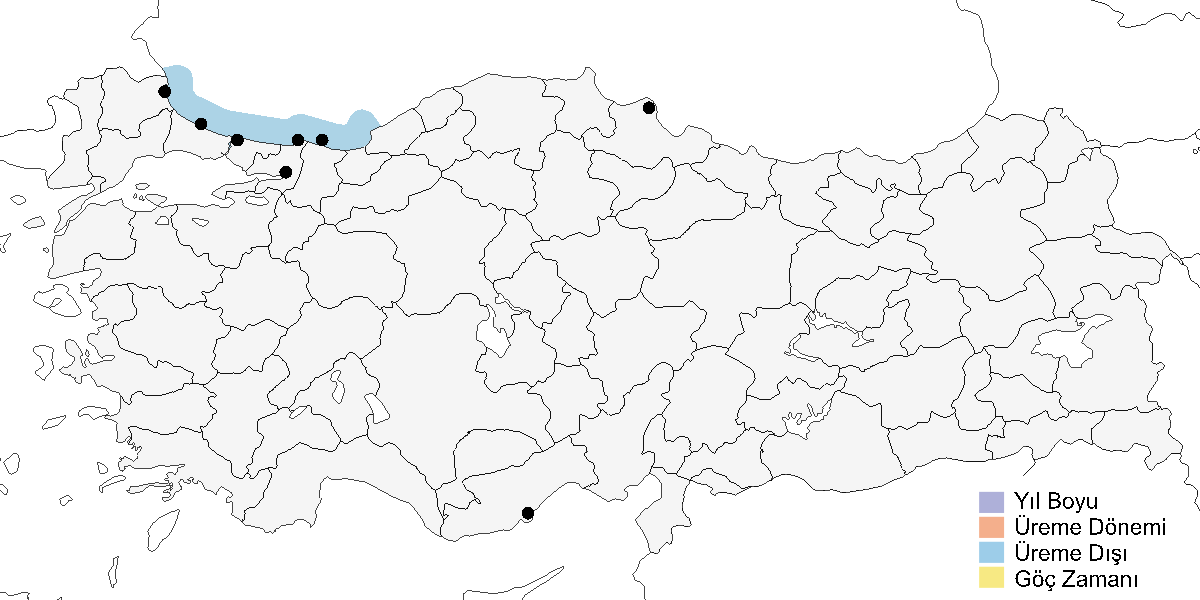
\includegraphics{images/harita_Somateria mollissima.png}

\textbf{Üreme}

Türkiye'de yuvalamaz. Ukrayna'daki koloni insan eliyle oluşturulmuş,
kolonideki kuşlar zamanlar doğallaşmıştır. Doğal yuvalama alanı Kuzey
Atlantik, Kuzey Buz Denizi ve Bering Boğazı'dır.

\textbf{Alttürler ve Sınıflandırma}

Ülkede gözlenen alttür nominat \emph{mollissima} (Kuzeybatı Avrupa)
alttürüdür.

\section{Kadife Ördek}\label{kadife-uxf6rdek}

\emph{Melanitta fusca}, Velvet Scoter

\textbf{\emph{Türkiye'de üreyen nüfus yok olmuştur. Karadeniz kıyılarına
az sayıda kışlar.}}

Doğu Anadolu'da az sayılarda kaydedilen çok lokal bir yaz konuğu idi. Az
sayıda yüksek irtifa göllerinde 3000 m'nin üstünde üremiş olduğu
düşünülür. Aktaş Gölü (Ardahan) kesin olarak ürediği tek alandır. 3 Ekim
1980'de 100 birey (Ven, 1980) ve 14-15 Temmuz 1994'te aralarında
gençlerin de bulunduğu 725 birey (Yarar, 1995) kaydedilmiştir.

Geçmişte Nemrut Dağı'ndaki (Tatvan) krater gölünde 20 çifte ürediği
düşünülmüştür. Ağrı Balık Gölü'nde geçmişte ürediği sanılmış, ancak
görünüşe göre Haziran 2001'de artık üremediğine karar kılınmıştır.
Çıldır Gölü'nde ürediği güçlü şekilde şüphelenilmiş, ancak teyit
edilmemiştir. Kars Aygır Gölü ve Muş Nazik Gölü'nde azami 32 birey yazı
geçirmiştir. Doğu Karadeniz kıyılarında kışlayan bireylerin yaz
aylarında da kaldığı gözlenmiştir.

Gürcistan'da yuvalamaya devam eden bireyler Karadeniz kıyılarına az
sayıda kışlar. Orta ve Doğu Karadeniz boyunca az sayıda kışlar. 1995
Aralık sonunda Yeşilırmak Deltası'nda 870 birey en yüksek kayıttır.
Nadir olarak Batı Karadeniz, Marmara'da ve güneyde Akdeniz kıyısında
kışlamıştır. Ocak 1970'de Burdur Gölü'nde 27 birey, Şubat 1966'da Mogan
Gölü'nde ve Ocak 2005'te Hazar Gölü'nde kaydedilmiştir. Son yıllarda
kaydedilen 50 birey.

4 Şubat 1917'de İstanbul Zeytinburnu açıklarında gözlenen iki birey ülke
için ilk kayıttır.

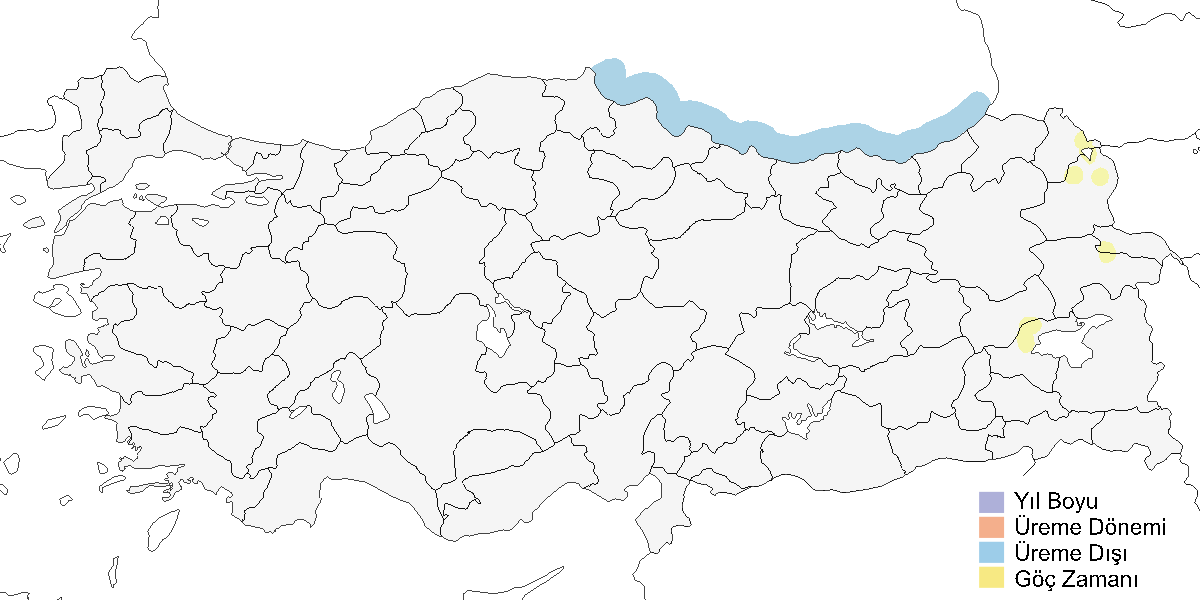
\includegraphics{images/harita_Melanitta fusca.png}

\textbf{Üreme}

\textbf{Yuvalama Alanı:} Doğu Anadolu'daki iki ya da üç yüksek irtifa
gölünde üremiştir. Tüm çabalara rağmen Türkiye'de yuvası bulunamamıştır.
Şu anda Kafkasya popülasyonu sadece Gürcistan'da bir gölde
yuvalamaktadır.\\
\textbf{Yuvası:} Türkiye'de yuva bulunmamıştır ancak diğer yerlerde
yoğun bitki örtüsünün içine gizlenmiş şekilde yerde ve genellikle
göllerdeki adalarda yuva yapar.\\
\textbf{Yumurta sayısı:} Olağan yumurta sayısı 7-10'dur.\\
\textbf{Üreme dönemi:} Eski gözlemlere göre temmuz ve ağustos ayında
yuvalamıştır. \textbf{DOA}. 10 Temmuz 1967'de Nemrut Dağı'ndaki krater
gölünde iki, yedi ve dokuz hav tüylü küçük yavru ile birlikte üç dişi ve
20 Ağustos 1967'de Balık Gölü'nde dört, beş ve altı yavrulu üç dişi
kaydedilmiştir (Vielliard, 1968). Küçük ördeklerin sadece yaklaşık bir
haftalık olduğu varsayılırsa yumurtlamanın haziranın ilk günlerinde
olduğu anlaşılmaktadır. 23 Ağustos 1972'de Nemrut Dağı'nda gözlenen
hemen hemen yarı gelişmiş yedi yavrulu bir dişi, yumurtlamanın haziranın
son haftasında olduğunu göstermektedir. 9 Temmuz 1985'te Nemrut Dağı'nda
beş çift ve iki genç birey gözlenmiştir. Son zamanlara ait bir üreme
kaydı yoktur ve 9 Haziran 2001'de Balık Gölü'ndeki adada yapılan
kapsamlı araştırmada ne yuva bulunmuş ne de erişkin görülmüştür.

\textbf{Alttürler ve Sınıflandırma}

Monotipik bir türdür. Eskiden Amerika ve Doğu Sibirya'da yaşayan Ak
Kanatlı Kadife Ördek \emph{Melanitta deglandi} ile aynı tür olarak kabul
ediliyordu.

\section{Kara Ördek}\label{kara-uxf6rdek}

\emph{Melanitta nigra,} Common Scoter

\textbf{\emph{Nadir kış konuğudur.}}

Karadeniz'de çoğunlukla eylül ve mart arasında çok az sayıda kaydedilen
kış göçmenidir. Düzenli olarak sadece Kızılırmak ve Yeşilırmak
deltalarının açıklarında 20 birey kışlamaktadır. Karadeniz kıyısında
toplam 20'den fazla kaydı vardır. Marmara ve Ege'de çok nadirdir,
Akdeniz'de sadece bir kere kaydedilmiştir.

9 Nisan 1967'de Kocaçay Deltası'nda kaydedilen bir birey ülke için kabul
edilebilir ilk kayıttır (OST, 1969). Öncesinde Ege'de nadir bir kış
göçmeni olduğundan (Krüper, 1875) ve İstanbul Boğazı ile Ceyhan
Deltası'ndaki şüpheli kayıtlardan (Kumerloeve, 1961) bahsedilmiştir.

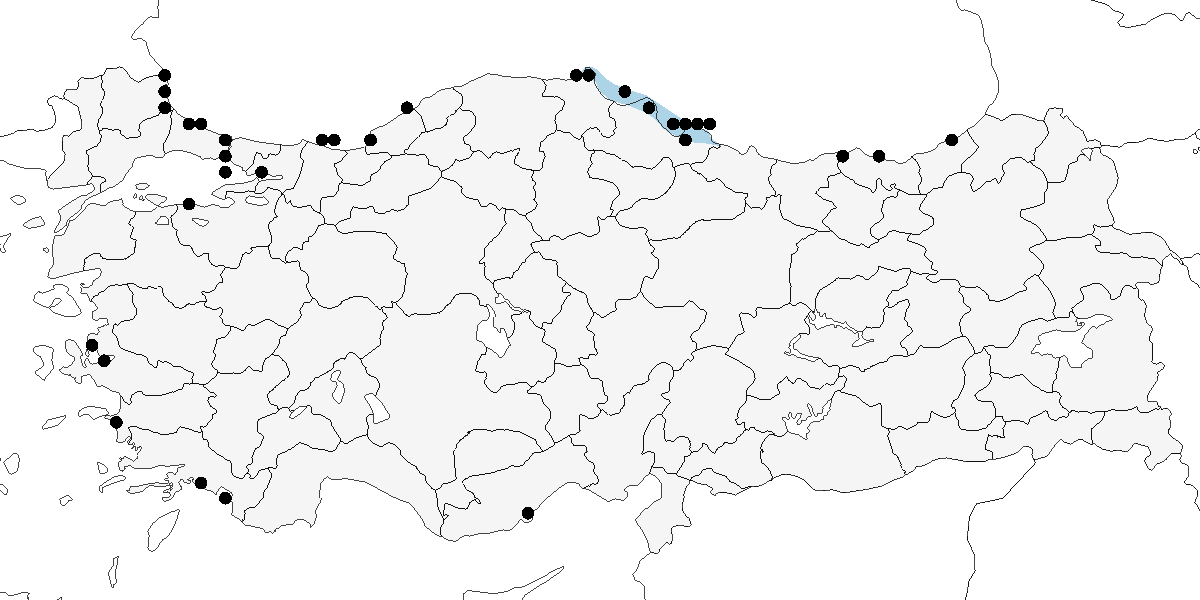
\includegraphics{images/harita_Melanitta nigra.png}

\textbf{Üreme}

Türkiye'de yuvalamaz. Avrasya'nın kuzeyinde yuvalar.

\textbf{Alttürler ve Sınıflandırma}

Monotipik bir türdür.

\section{Telkuyruk}\label{telkuyruk}

\emph{Clangula hyemalis}, Long-tailed Duck

\textbf{\emph{Nadir kış konuğudur.}}

Şubat 1893'te İstanbul (Büyük?) Çekmece'de, Alléon tarafından toplanan
genç bir dişi ülke için ilk kayıttır ve bu örnek Sofya Doğa Tarihi
Müzesi'nde görülebilir. Ardından, 13 Kasım 1968'de İzmit'te genç bir
birey kaydedilmiştir (OST, 1975). Göksu Deltası Paradeniz Gölü'nde 1-2
Ocak 1986'da bir birey ve 5 Ocak 1989'da bir dişi (Kasparek, 1990)
görülmüştür. Sakarya Nehri ağzında 18 Şubat 2004'te (Balmer and Betton,
2004b); 26 Şubat 2006'da Fırtına Nehri'nin ağzında birer birey
fotoğraflanmıştır. En güncel kayıtlara göre; 7-19 Ocak 2008'de
İğneada'da erişkin bir dişi, 13 Şubat 2008'de Kıyıköy'de bir erkek, 10
Aralık 2008'de İğneada'da bir birey (on üçüncü kaydı) ve 28 Mart 2009'da
Enez'de bir birey (on dördüncü kaydı) görülmüştür (Kirwan and Özen,
2014).

İstisnai olarak, Van Gölü'nden 1977 ile 1987 arasında mayıs ve haziran
aylarında yaz kayıtları mevcuttur. 10 Haziran 1977'de Gevaş'ın batısında
Horkum'da iki birey ve Tatvan ile Ahlat arasında üç birey (Beaman,
1986), 22 Mayıs 1985'te Van'ın güneybatısında bir erkek (Martins, 1989),
9 Haziran 1987'de Van Sazlığı'nda bir erkek ve 22 Haziran 1987'de Van'ın
10 km güneyinde bir birey (Kirwan and Martins, 1994) kaydedilmiştir.

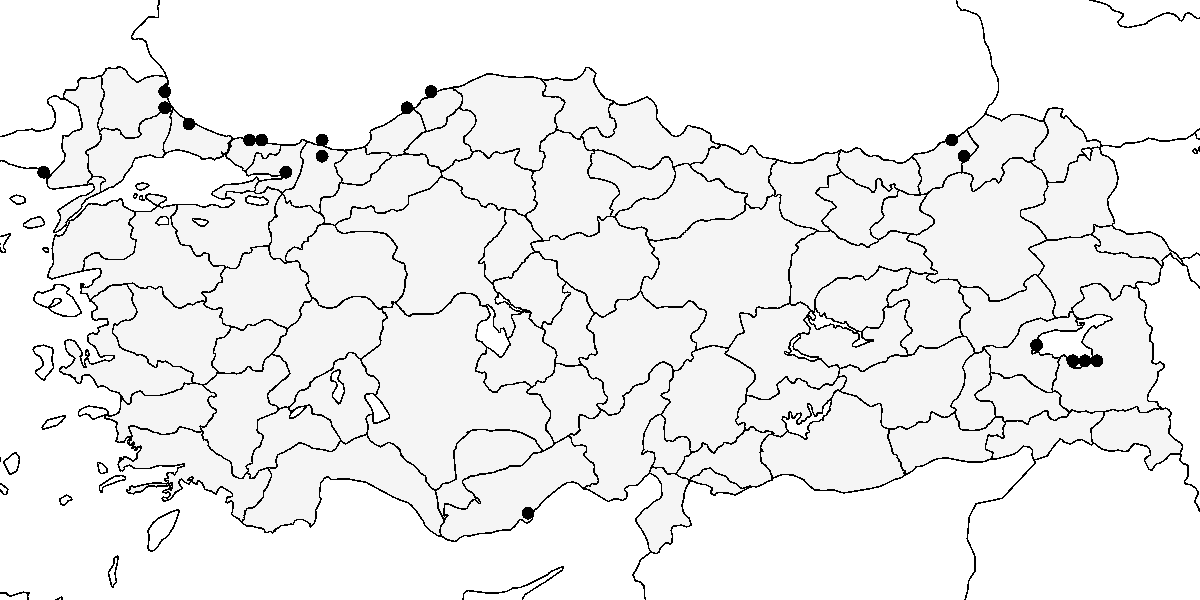
\includegraphics{images/harita_Clangula hyemalis.png}

\textbf{Üreme}

Türkiye'de yuvalamaz. Kuzey İskandinavya dağlarında ve Rusya ve Kuzey
Amerika'nın tundra kuşağında yuvalar.

\textbf{Alttürler ve Sınıflandırma}

Monotipik bir türdür.

\section{Altıngöz}\label{altux131nguxf6z}

\emph{Bucephala clangula,} Common Goldeneye

\textbf{\emph{Nispeten yaygın ve az sayıda kış konuğudur.}}

Karadeniz, Marmara ve Ege'nin kıyı bölgelerinde ve daha nadir olarak iç
bölgelerdeki sulakalanlarda ekim sonu ve nisan sonu arasında nadir bir
kış konuğudur. En düzenli olarak Marmara ve Karadeniz bölgelerinde
görülür. Kışın ülke çapında görülen kuş sayısı nadiren 100 bireyi geçer.
3 Şubat 1992'de Kızılırmak Deltası'nın açıklarında gözlenen 200 birey,
kaydedilen en yüksek sayıdır. 2005-06 kışında Gediz Deltası'nda 72
birey, 3 Şubat 2002'de Gala Gölü'nde 60 birey sayılmıştır (Demirci,
2002). Son yıllarda ilkbahar sonunda Doğu Karadeniz'de kaydedilmiştir.

1977 ile 1993 yılları arasında Doğu Anadolu'da, çoğunluğu Van Gölü'nde
olmak üzere, bir dizi yaz kaydı vardır ve bu kayıtlarda bazen birden
fazla birey gözlenmiştir. Bu kayıtlar, yakınlarda üreyen bir
popülasyonun ihtimalini düşündürmüştür (Kasparek, 1992).

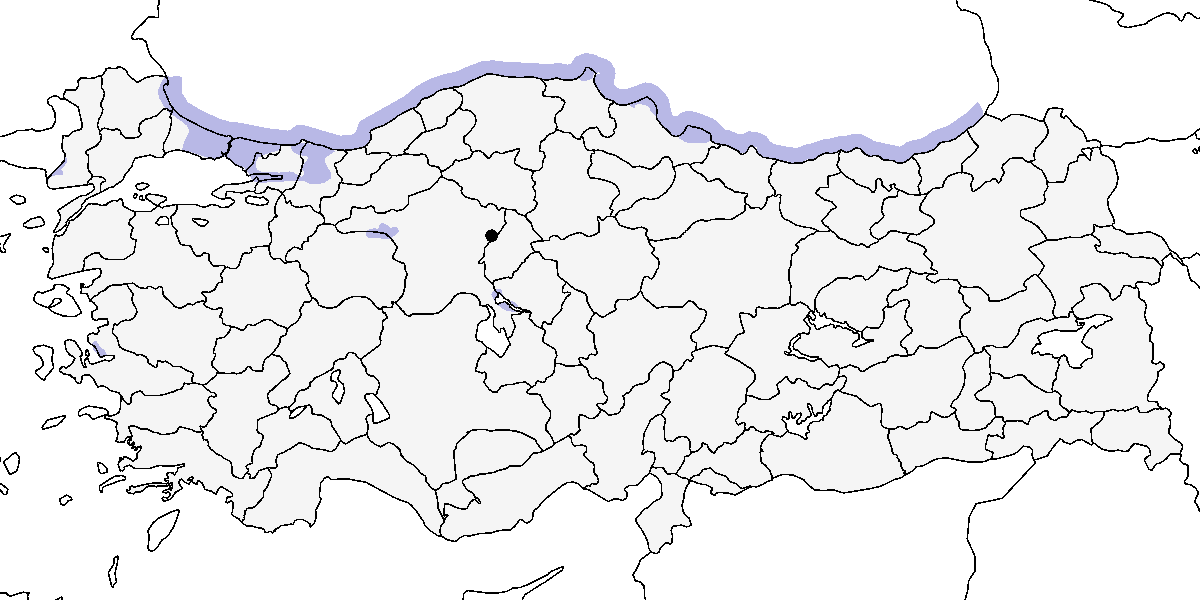
\includegraphics{images/harita_Bucephala clangula.png}

\textbf{Üreme}

Türkiye'de yuvalamaz. Avrasya ve Kuzey Amerika'nın kuzeyinde yuvalar.

\textbf{Alttürler ve Sınıflandırma}

Türkiye'de nominat alttürü bulunur.

\section{Sütlabi}\label{suxfctlabi}

\emph{Mergellus albellus,} Smew

\textbf{\emph{Kuzey bölgelerine az sayıda gelen bir kış konuğudur.}}

Kasımdan nisan ortasına kadar ülkenin batı ve orta bölgelerindeki
sulakalanlarda ve kıyılarda tipik olarak nadir ve muhtemelen düzensiz
bir kış konuğudur. En çok Marmara, Karadeniz ve İç Anadolu'da
kaydedilir. Her kış genellikle 100 bireyden daha azdır. Uluabat Gölü'nde
1967'de 300, 1969-70'de 1300, 1973'te 555, 1989'da 111 ve 1995'te 248
birey kaydedilmiştir. 1992'de Manyas Gölü'nde 102 ve 1993'te
Büyükçekmece'de 79 birey kışlamıştır.

Nisan 1987 sonunda Diyarbakır'da kaydedilmiştir. Doğu ve Güneydoğu
Anadolu'da oluşturulan büyük baraj göllerinde gözlenmesi beklenebilir.
Ocak 1979'da Irak Razzaza Gölü'nde gözlenen 1000'den fazla birey (Scott
and Carp, 1982), daha güneyde yüksek sayılarda kaydedilebileceğini
göstermektedir.

Ancak ne tuhaftır ki, türün ilk keşfi Strickland tarafından İzmir'den
alınan iki örnek ile yapılmıştır. Cambridge Üniversitesi Zooloji
Müzesi'ndeki koleksiyonda bulunan bu örnekler, 6 Ocak 1836'da alınan bir
erkek ve aynı yıl şubat ayında alınan bir dişiye aittir. 1946-48
yıllarında Çatalağzı açıklarında (Zonguldak) oldukça bol olduğu
gözlenmiştir (Ogilvie, 1954).

11 Haziran 1969'da Eymir Gölü'nde (Ankara) bir erkek (OST, 1972), 27
Haziran 1987'de Göründü'de (Van) bir dişi (Kirwan and Martins, 1994) ve
27 Mayıs 1995'te Uluabat Gölü'nde bir erkek ve iki dişi (Kirwan and
Martins, 2000) olmak üzere yazın üç defa kaydedilmiştir.

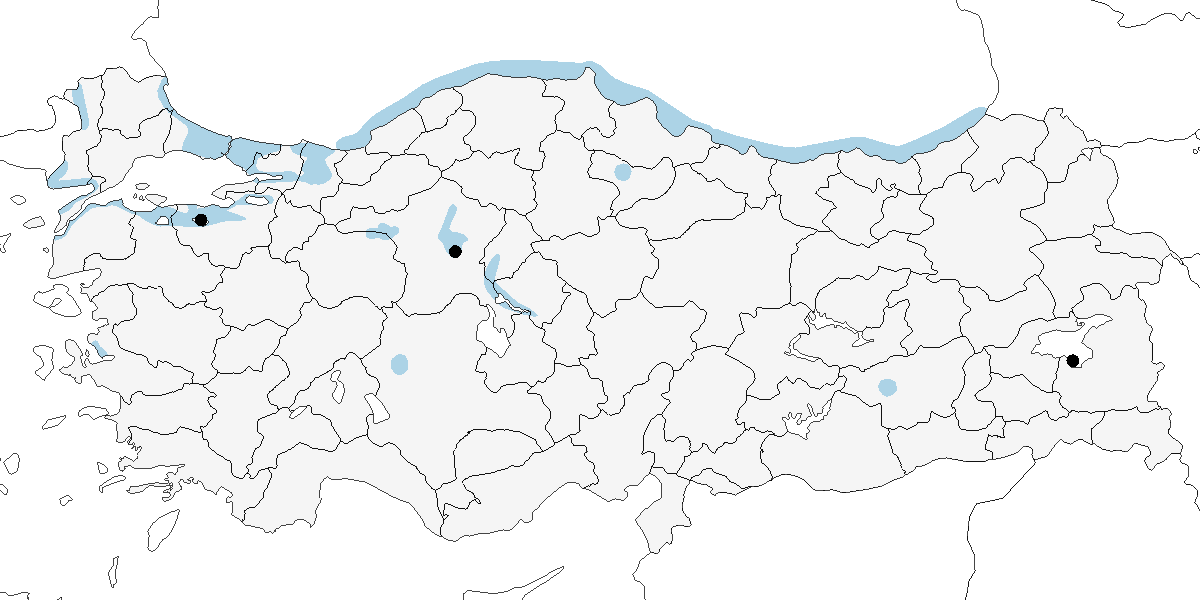
\includegraphics{images/harita_Mergellus albellus.png}

\textbf{Üreme}

Türkiye'de yuvalamaz. Avrasya'nın kuzeyinde yuvalar.

\textbf{Alttürler ve Sınıflandırma}

Monotipik bir türdür. Türkiye'de tanımlanmıştır.

\section{Büyük Tarakdiş}\label{buxfcyuxfck-tarakdiux15f}

\emph{Mergus merganser,} Common Merganser

\textbf{\emph{Nadir kış konuğudur.}}

Özellikle Marmara ve Karadeniz bölgelerinde az sayıda kaydedilen nadir
bir kış konuğudur. 1997-2007 arasında artan gözlemci aktivitesine karşın
sadece 10 kere kaydedilmiştir (Kirwan et al., 2003). Genellikle kıyısal
sulakalanlarda görülür ve en düzenli olarak Kızılırmak ve Yeşilırmak
deltalarında kaydedilir. Kızılırmak Deltası'nda görüldüğü en geç tarih
20 Mayıs'tır.

Doğu Anadolu'da şubat ve martta iki defa, yazın ise üç kere
gözlenmiştir; 11 Haziran 1970'de Pasinler ile Horasan arasında Aras
Nehri üzerinde bir çift, 7 Haziran 1986'da Van Gölü'nde bir birey ve 29
Haziran 1988'de Bendimahi Deltası'nda bir dişi ya da genç birey
kaydedilmiştir. Kurutulmadan önce Sevan Gölü (Ermenistan) havzasında
üreyen bir tür olduğu düşünülmüş, ancak ürediğine dair bir kanıt elde
edilmemiştir (Adamian and Klem, 1999).

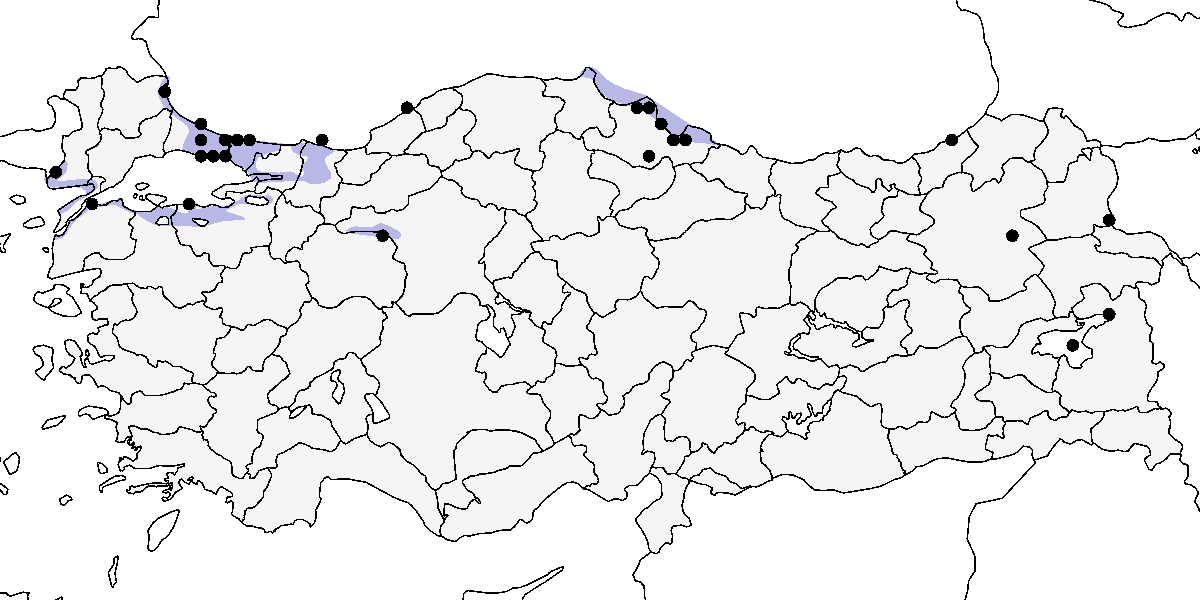
\includegraphics{images/harita_Mergus merganser.png}

\textbf{Üreme}

Türkiye'de yuvalamaz. Avrasya ve Kuzey Amerika'nın kuzeyinde yuvalar.

\textbf{Alttürler ve Sınıflandırma}

Türkiye'de nominat alttürü bulunur.

\section{Tarakdiş}\label{tarakdiux15f}

\emph{Mergus serrator}, Red-breasted Merganser

\textbf{\emph{Nispeten lokal olarak ve orta sayılarda görülen bir kış
konuğudur.}}

Kıyısal alanlarda ekim sonu ve nisan sonu arasında kaydedilen kış
göçmenidir. En çok sayıda Doğu Karadeniz, Marmara ve Ege'de kaydedilir.
Gediz Deltası'nda düzenli olarak yaklaşık 100 birey konaklar; Şubat
1996'da 397 birey sayılmıştır. Büyük Menderes Deltası'nda Şubat 1993'te
67 birey ve Yumurtalık'ta 44 birey kaydedilmiştir. Ege ve Doğu
Akdeniz'deki alanlarda düzenli olarak önemli sayılarda kışlar (Eken,
1997d). Akdeniz kıyılarında seyrek olsa da Kıbrıs'ta oldukça düzenli bir
türdür.

20-21 Mayıs 1994'te Göksu Deltası'nda geç kalmış bir birey
kaydedilmiştir (Birdquest Newsletter 23: 59). Tek yaz kaydı 11 Haziran
1964'te Amik Gölü'nde (Antakya) kaydedilen yedi veya sekiz bireydir
(Kumerloeve, 1966-67).

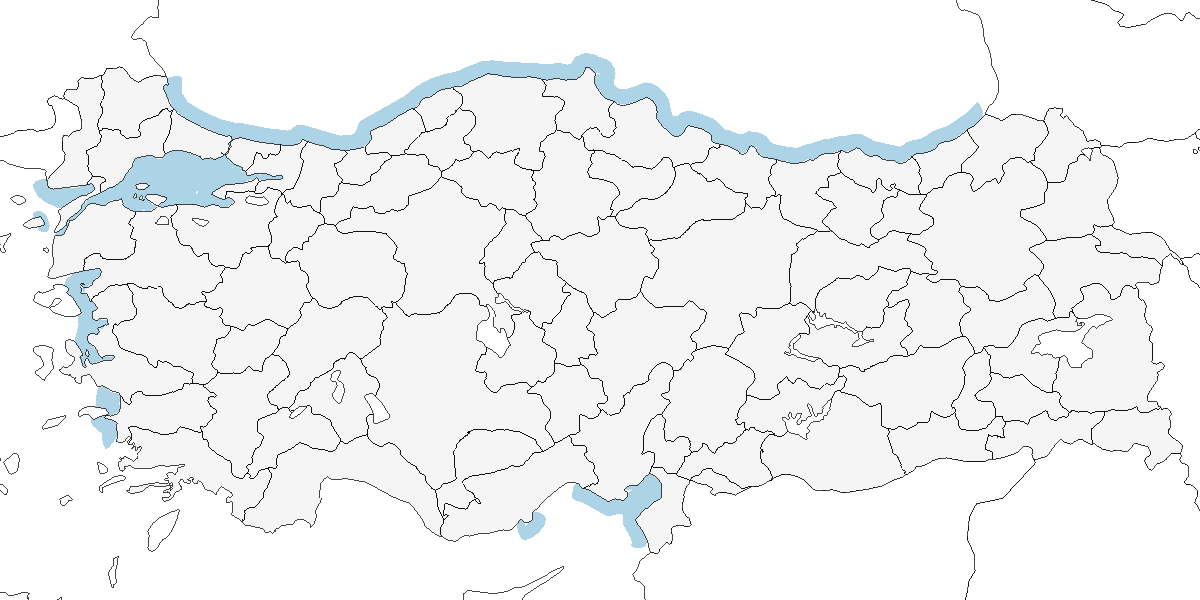
\includegraphics{images/harita_Mergus serrator.png}

\textbf{Üreme}

Türkiye'de yuvalamaz. Avrasya ve Kuzey Amerika'nın kuzeyinde yuvalar.

\textbf{Alttürler ve Sınıflandırma}

Monotipik bir türdür.

\section{Dikkuyruk}\label{dikkuyruk}

\emph{Oxyura leucocephala,} White-headed Duck

\textbf{\emph{Lokal olarak az sayıda üreyen yaz konuğu, nispeten yaygın
ve yüksek sayıda bulunabilen geçit türü ve kış konuğudur.}}

İç Anadolu ve Doğu Anadolu'da tatlı veya acı (sodalı), sığ ve ötrofik
göllerdeki yoğun sazlık sulakalanlarda az ila orta sayıda yuvalar. Van
Gölü çevresinde ve Kars'taki küçük sulakalanlarda ürediği teyit
edilmiştir. Doğu Anadolu'daki diğer alanlardaki üreme durumu
belirsizdir. Niğde Akkaya Barajı'nda üremiştir (Kirwan, 1994). Üreme
döneminde kaydedildiği Karadeniz Bölgesi'ndeki bazı alanlarda
yuvalayabilir. Doğu Akdeniz sulakalanlarında yaz kayıtları, üremeyen
bireylere aittir.

1980'lerin sonu ve 1990'ların başı arasında dört kilit alanda (Ereğli
Sazlığı, Hotamış Gölü, Sultansazlığı ve Kulu Gölü) üreyen İç Anadolu
popülasyonu muhtemelen 150 çiftin üzerindeydi (Robinson and Can, 1998).
Ancak 1990'ların ortasında Ereğli Sazlığı ve Hotamış Gölü'nün
kurumasıyla sayıları azalmış, Kulu Gölü'nde üremez olmuştur (Richardson,
2003). Kozanlı Gökgöl ve Uyuz Gölü'nde az sayıda üremeye devam
etmektedir.

Mart ile mayıs başı arasında birçok alanda geçiş sırasında gözlenir. 23
Mart 1992'de Kızılırmak Deltası'nda 1246 birey ve Mart 1990'da Ereğli
Sazlığı'nda 508 birey toplanmıştır. Mayıs ve haziran arasında toplanan
sürüler muhtemelen üreme alanlarına dağılacak kuşlardan oluşur. Temmuz
ve eylül arasında toplanan sürüler ise üreme sonrası dağılmaya ve göç
almaya işaret eder. Temmuzda Kulu Gölü'nde 500 birey ve ağustosta Sodalı
Gölü'nde 600-1000 birey kaydedilmiştir.

Kışın Akdeniz'deki birkaç sulak alanda yüksek sayıda, İç Anadolu'da
genellikle daha az sayıda kaydedilir. Batı ve orta bölgelerindeki diğer
yerlerde ise daha nadiren, özellikle sert hava koşullarında kaydedilir.
Karadeniz Bölgesi'nde düzensiz olarak yüksek sayılarda kışlar. Bir dönem
dünya popülasyonunun \%50'sinden fazlasının Burdur Gölü'nde kışladığı
düşünülmüştür; buradaki sayımlarda 1987'de 6400, 1988'de 9230, 1989'da
6700 ve 1991'de 10.927 birey kaydedilmiştir (Green and Anstey, 1992).
Ancak 1992 sonrasında sayılarda azalma görülmüş; 1992'de 3264, 1993'de
3010 ve 1994'de 3337 birey sayılmıştır. Bu sayımlar son derece hassas
olup, eş zamanlı üç ekip tarafından ideal hava koşullarında
gerçekleştirilmiştir. Burdur Gölü'nde 1993'te 1991'e göre daha az genç
bireyin sayılması, daha düşük üreme başarısını gösterebilir. Bir
ihtimal, Kazakistan ve çevre ülkelerdeki üreyen nüfustaki azalış,
Türkiye'deki kışlama nüfusunun azalmasını açıklayabilir. Bu azalmada
şüphesiz kaçak avcılığın da payı vardır; 1992-93 kışında Burdur Gölü'nde
1000'den fazlasının vurulduğu tahmin edilmiştir. Ayrıca son yıllarda
Burdur Gölü'nün kuruma sürecinin başlaması ve tuzluluğun artması da bir
etken olabilir.

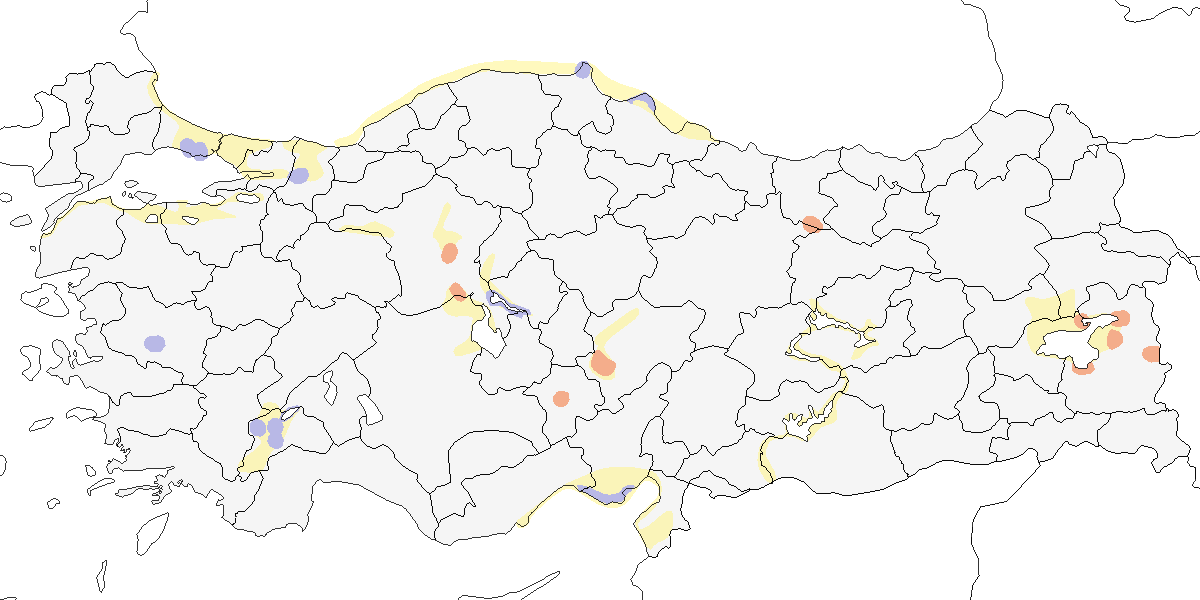
\includegraphics{images/harita_Oxyura leucocephala.png}

\textbf{Üreme}

\textbf{Yuvalama Alanı:} Çoğunlukla büyük sulak alanların yakınlarında
genellikle 10 hektardan küçük ve 2 metreden sığ, sualtı vejetasyonu bol
ve su aynalarının bulunduğu geniş sazlıklara sahip tatlı su göllerinde
ya da sodalı göllerde ürer (Anstey, 1989). Aynı alanda birkaç çift
üreyebilir.\\
\textbf{Yuvası:} Yuva, ölü saz gövdeleri ile diğer sucul bitkilerin
düzgün bir kâse oluşturacak şekilde örülmesi ile oluşturulmuş, birkaç
tutam açık gri tüy ile astarlanmış dayanıklı bir yapıdır.\\
\textbf{Yumurta sayısı:} Bir yuvada en fazla 10 yumurta kaydedilmiştir.
19 Haziran 2004'te aynı gölde diz boyu derinliğindeki suda yoğun bir
sazlığın içinde iyice gizlenmiş bir şekilde suyun üzerinde dikey
sazların dibine tutturularak yapılmış bir yuvada on yumurtalı
tamamlanmış bir kuluçka bulunmuştur. Diğer yerlerde olağan yumurta
sayısı 5-12'dir. Dikkuyruk, vücut ölçülerine göre son derece büyük ve
ağır yumurtalar koyar; yuva bu ağırlık nedeniyle suya batabilir.\\
\textbf{Üreme dönemi:} Mayıs başı ve temmuz başı arasında yumurta koyar.
Eylül sonuna kadar yavrular görülebilir. \textbf{İÇA.} 13 Temmuz 1987'de
Kulu Gölü'ndeki sazlıkların içindeki yuvada yedi yumurta gözlenmiştir;
muhtemelen dişinin kuluçkaya ara vermesi nedeniyle yuva ve yumurtalar
kısmen su altında kalmıştır (Anstey, 1989). Üreme kayıtlarının çoğu 3-10
yavrudan oluşan gruplardır: İç Anadolu'daki en erken kayıt, 5 Haziran
1975'te Kulu Gölü'nde gözlenen üç büyük ve üç hav tüylü yavrudur; bu
durum yumurtlamanın mayıs başında olduğunu gösterir. 6 Ağustos 1972'de
(kurutulmuş) Gönenç Gölü'nde 20 günlük beşer yavrularıyla iki dişi ve
dört günlük altı yavrulu bir dişi gözlenmiştir; bu kayıtlar
yumurtlamanın haziran ortası ile temmuz başında olduğunu göstermektedir.
İç Anadolu'da, temmuz ve ağustosta birçok yavrulu aile kaydedilmiştir.
\textbf{DOA.} Haziran-eylül ayları arasında Van Gölü'nde 9 Haziran 1987
ve 14 Haziran 1990'da gözlenen genç bireyler, yumurtlamanın mayıs
ortasında olduğunu göstermektedir. Temmuz-ağustos arasındaki diğer
kayıtlar, yumurtlamanın haziran ortasında başladığını düşündürmektedir.
Erçek Gölü yakınlarındaki küçük bir gölün ortasında dikey sazlardan
oluşan bir adada bir yuva bulunmuştur; sucul bitkiler kullanılarak
sazların dibine yapılmış olan yuvada 11 Haziran 2001'de iki yumurta
olduğu, kuluçkanın henüz tamamlanmadığı gözlenmiştir; alanda sekiz erkek
ve yedi dişi birey kaydedilmiştir. Ancak oldukça kapsamlı bir araştırma
yapılmasına rağmen başka bir yuva bulunmaması, üremenin henüz tam
anlamıyla başlamadığını göstermektedir.

\textbf{Alttürler ve Sınıflandırma}

Monotipik bir türdür.

\bookmarksetup{startatroot}

\chapter*{Kaynakça}\label{kaynakuxe7a}
\addcontentsline{toc}{chapter}{Kaynakça}

\markboth{Kaynakça}{Kaynakça}

\phantomsection\label{refs}
\begin{CSLReferences}{1}{0}
\bibitem[\citeproctext]{ref-adamian1999}
Adamian, M.S., Klem, D., 1999. {Handbook of the Birds of Armenia}.
American University of Armenia, Oakland.

\bibitem[\citeproctext]{ref-adizel1998}
Adızel, Ö., 1998. {Van Gölü Havzası Ornithofaunası Üzerine Araştırmalar}
(PhD thesis). Van 100 Yıl Üniversitesi.

\bibitem[\citeproctext]{ref-alleon1880}
Alléon, C.A., 1880. {Catalogue des Oiseaux Observés Aux Environs de
Constantinople}. Bull. Zool. Soc. France 5, 80--116.

\bibitem[\citeproctext]{ref-anstey1989}
Anstey, S., 1989. {The Status and Conservation of the White-headed Duck
({Oxyura leucocephala})}. IWRB (Spec. Publ. No. 10), Slimbridge.

\bibitem[\citeproctext]{ref-aou2000}
(AOU), A.O.U., 2000. {Forty-second supplement to the American
Ornithologists' Union Check-list of North American Birds}. Auk 117,
847--858.

\bibitem[\citeproctext]{ref-balkiz2009}
Balkız, Ö., Kartal, E., Parmak, B., Onmuş, O., Sıkı, M., Aydın, A.,
2009. {5. Flamingo Halkalama Raporu}. Doğa Derneği.

\bibitem[\citeproctext]{ref-balmer2004b}
Balmer, D., Betton, K., 2004b. {Around the region}. Sandgrouse 26,
160--168.

\bibitem[\citeproctext]{ref-baris2005}
Barış, S., Erciyas, K., Gürsoy, A., Özsemir, C., Nowakowski, J.K., 2005.
{Cernek: a new bird ringing station in Turkey}. The Ring 27, 113--120.

\bibitem[\citeproctext]{ref-baumgart1995}
Baumgart, W., Kasparek, M., Stephan, B., 1995. {Die Vögel Syriens: eine
Übersicht}. Kasparek Verlag, Heidelberg.

\bibitem[\citeproctext]{ref-beaman1986}
Beaman, M., 1986. {Turkey Bird Report 1976--81}. Sandgrouse 8, 1--41.

\bibitem[\citeproctext]{ref-beaman1977}
Beaman, M., 1977. {Further news on raptor migration in the north east}.
Orn. Soc. Turkey Bull. 15.

\bibitem[\citeproctext]{ref-beaman1977a}
Beaman, M., Porter, R.F., 1977. {A {``new''} raptor migration route
through NE Turkey}. Orn. Soc. Turkey Bull. 14, 2--5.

\bibitem[\citeproctext]{ref-boyla1998a}
Boyla, K.A., Eken, G., 1998. {Remarkable sightings}. Turna 1, 35--40.

\bibitem[\citeproctext]{ref-boyla2018}
Boyla, K.A., Sinav, L., Dizdaroğlu, D.E., 2018. {Türkiye Üreyen Kuş
Atlası}. WWF-Türkiye, Doğal Hayatı Koruma Vakfı, İstanbul.

\bibitem[\citeproctext]{ref-brazil2003}
Brazil, M.A., 2003. {The Whooper Swan}. T. \& A. D. Poyser, London.

\bibitem[\citeproctext]{ref-caglayan2005}
Çağlayan, E., Kılıç, D.T., Per, E., Gem, E., 2005. {Türkiye Kış Ortası
Sukuşu Sayımları 2005}. Doğa Derneği, Ankara.

\bibitem[\citeproctext]{ref-demirci2002}
Demirci, B., 2002. {Toygardan Kayıtlar (Ocak--Mart 2002)}. Kuşçu Bulteni
11, 6--7.

\bibitem[\citeproctext]{ref-dogalhayati1992}
DHKD, 1992. {Results of the International Waterfowl Census Turkey 1992.
Bird Section Report No. 6}. Doğal Hayatı Koruma Derneği, Istanbul.

\bibitem[\citeproctext]{ref-dogalhayati1999}
DHKD, D.H.K.D., 1999. {Results of the International Waterfowl Census
Turkey 1999. Biodiversity Programme Report No. 10}. Istanbul.

\bibitem[\citeproctext]{ref-dogalhayati1993}
DHKD, D.H.K.D., 1993. {Results of the International Waterfowl Census
Turkey 1993. Bird Section Report No. 7}. Istanbul.

\bibitem[\citeproctext]{ref-dijksen1988}
Dijksen, L.J., Kasparek, M., 1988. {The Birds of Acıgöl}. Kasparek
Verlag, Heidelberg.

\bibitem[\citeproctext]{ref-dijksen1985}
Dijksen, L.J., Kasparek, M., 1985. {The Birds of Kızılirmak Delta}.
Kasparek Verlag, Heidelberg.

\bibitem[\citeproctext]{ref-eken1997d}
Eken, G., 1997d. {The wintering populations of some waterbird species on
the Mediterranean coastline of Turkey} 61--69.

\bibitem[\citeproctext]{ref-eken1997a}
Eken, G., 1997a. {The breeding populations of some species of waterbirds
at Gediz Delta, western Turkey}. Zool. Middle East 14, 53--68.

\bibitem[\citeproctext]{ref-emirogullari_inprep}
Emirogullari, E.F., Sonmez, E., Özesmi, S., Özesmi, U., n.d. {Status of
Ruddy Shelduck Tadorna ferruginea in Turkey}.

\bibitem[\citeproctext]{ref-ertan1996}
Ertan, K.T., 1996. {The Birds of Kocaçay Delta}. Birds of Turkey 12.

\bibitem[\citeproctext]{ref-green1993}
Green, A.J., 1993. {The Status and Conservation of the Marbled Teal
Marmaronetta angustirostris}. IWRB (Spec. Publ. No. 23), Slimbridge.

\bibitem[\citeproctext]{ref-green1992}
Green, A.J., Anstey, S., 1992. {The status of the White-headed Duck
\emph{Oxyura leucocephala}}. Bird Conserv. Intern. 2, 185--200.

\bibitem[\citeproctext]{ref-grimmett1989}
Grimmett, R.F.A., Jones, T.A., 1989. {Important Bird Areas in Europe}.
International Council for Bird Preservation, Cambridge.

\bibitem[\citeproctext]{ref-handrinos1997}
Handrinos, G., Akriotis, T., 1997. {The Birds of Greece}. Christopher
Helm, London.

\bibitem[\citeproctext]{ref-hustings1994}
Hustings, F., Dijk, K. van, 1994. {Bird Census in the Kizilirmak Delta,
Turkey, in Spring 1992}. WIWO (Report No. 45) Zeist.

\bibitem[\citeproctext]{ref-kasparek1992a}
Kasparek, M., 1992. {Die Vögel der Türkei: eine Übersicht}. Kasparek
Verlag, Heidelberg.

\bibitem[\citeproctext]{ref-kasparek1990a}
Kasparek, M., 1990. {Zum Vorkommen einiger in der Türkei seltener
Vogelarten}. Bonn. Zool. Beitr. 41, 181--202.

\bibitem[\citeproctext]{ref-kasparek1988a}
Kasparek, M., 1988. {Der Bafasee. Natur und Geschichte in der türkischen
Ägäis}. Kasparek Verlag, Heidelberg.

\bibitem[\citeproctext]{ref-kasparek1987a}
Kasparek, M., 1987. {The Birds of Kulu Gölü. Birds of Turkey 5}.
Kasparek Verlag, Heidelberg.

\bibitem[\citeproctext]{ref-kasparek1983}
Kasparek, M., Ven, J. van der, 1983. {The Birds of Erçek Gölü. Birds of
Turkey 1}. Kasparek Verlag, Heidelberg.

\bibitem[\citeproctext]{ref-kirwan1997a}
Kirwan, G.M., 1997b. {A list of bird specimens held in the Robert's
College, Bebek (Istanbul, Turkey) collection, with some comments on
Mathey-Dupraz (1920--24)}. Sandgrouse 19, 30--38.

\bibitem[\citeproctext]{ref-kirwan1997b}
Kirwan, G.M., 1997a. {The status of the Ferruginous Duck \emph{Aythya
nyroca} in Turkey}. Bird Conserv. Intern. 7, 345--356.

\bibitem[\citeproctext]{ref-kirwan1994b}
Kirwan, G.M., 1994. {The breeding status and distribution of the
White-headed Duck (\emph{Oxyura leucocephala}) on the Central Plateau,
Turkey}. Sandgrouse 16, 66--75.

\bibitem[\citeproctext]{ref-kirwan1993a}
Kirwan, G.M., 1993. {The Birds of Hotamış}. Birds of Turkey 9.

\bibitem[\citeproctext]{ref-kirwanmartins2000}
Kirwan, G.M., Martins, R.P., 2000. {Turkey Bird Report 1992--1996}.
Sandgrouse 22, 13--35.

\bibitem[\citeproctext]{ref-kirwanmartins1994}
Kirwan, G.M., Martins, R.P., 1994. {Turkey Bird Report 1987--91}.
Sandgrouse 16, 76--117.

\bibitem[\citeproctext]{ref-kirwan2014}
Kirwan, G.M., Özen, E., M., 2014. {Turkey Bird Report 2007--2011}.
Sandgrouse 36.

\bibitem[\citeproctext]{ref-kirwan2006apress}
Kirwan, G.M., Özen, M., Demirci, B.(compilers)., 2009. {Turkey Bird
Report 2002--06}. Sandgrouse 30.

\bibitem[\citeproctext]{ref-kirwan2003}
Kirwan, G.M., Özen, M., Kurt, B., Martins, R.P., 2003. {Turkey Bird
Report 1997--2001}. Sandgrouse 25, 8--31.

\bibitem[\citeproctext]{ref-kivit1994}
Kivit, H.A., Nijmeijer, H., Ovaa, A.(eds.)., 1994. {Wader and Waterfowl
Migration in the Çukurova Deltas, South Turkey, Spring 1990}. WIWO
(Report No. 48), Zeist.

\bibitem[\citeproctext]{ref-kilic1990}
Kılıç, A., Kasparek, M., 1990. {The Ereğli Marshes: assessment of their
biological importance and recommendations for conservation}. Unpubl.
report to International Council for Bird Preservation/World Wildlife
Fund.

\bibitem[\citeproctext]{ref-kruper1875}
Krüper, T., 1875. {Beitrag zur Ornithologie Kleinasiens}. J. Orn. 23,
258--285.

\bibitem[\citeproctext]{ref-kumerloeve1966d}
Kumerloeve, H., 1966. {Ergänzungen zur Avifauna Kleinasiens}. Bonn.
Zool. Beitr. 17, 257--259.

\bibitem[\citeproctext]{ref-kumerloeve1964a}
Kumerloeve, H., 1964. {Zur Sumpf- und Wasservogelfauna der Türkei}. J.
Orn. 105, 307--325.

\bibitem[\citeproctext]{ref-kumerloeve1963a}
Kumerloeve, H., 1963. {L'Avifaune du lac d'Antioche (Amik Gölü-Gölbasi)
et de ses alentours}. Alauda 30, 110--136, 161--211.

\bibitem[\citeproctext]{ref-kumerloeve1961}
Kumerloeve, H., 1961. {Zur Kenntnis der Avifauna Kleinasiens}. Bonn.
Zool. Beitr. 12, 1--318.

\bibitem[\citeproctext]{ref-kumerloeve1970a}
Kumerloeve, H., 1970a. {Zur Kenntnis der Avifauna Kleinasiens und der
europäischen Türkei (Ergänzungen -- Hinweise -- Fragestellungen)}.
Istanbul Fen. Fak. Mecm. B 35, 85--160.

\bibitem[\citeproctext]{ref-kumerloeve1967a}
Kumerloeve, H., 1967a. {Neue Beiträge zur Kenntnis der Avifauna Nordost-
und Ost-Kleinasiens}. Istanbul Üniv. Fen. Fak. Mecm. B 32, 79--213.

\bibitem[\citeproctext]{ref-kumerloeve1966-67}
Kumerloeve, H., 1966-67. {Migration et hivernage sur le Lac d'Antioche
(Amik Gölü, Hatay, Turquie); coup l'oeil sur son avifaune nidificatrice
actuelle}. Alauda 34, 299-308; 35: 1-19.

\bibitem[\citeproctext]{ref-magninyarar1997}
Magnin, G., Yarar, M., 1997. {Important Bird Areas in Turkey}. Doğal
Hayatı Koruma Derneği, Istanbul.

\bibitem[\citeproctext]{ref-makatsch1950}
Makatsch, W., 1950. {Die Vogelwelt Macedoniens}. Leipzig.

\bibitem[\citeproctext]{ref-martins1989}
Martins, R.P., 1989. {Turkey Bird Report 1982--86}. Sandgrouse 11,
1--41.

\bibitem[\citeproctext]{ref-matheydupraz1920}
Mathey-Dupraz, A., 1920--24. {Notes ornithologiques de la région du
Bosphore}. Orn. Beob. 17, 25--29, 108-110; 18: 25-27, 38--41, 55--58,
101--104, 137--139, 157--158, 183-187; 19: 22-25, 41--43, 58--61,
116--119, 156-159; 20: 9-12, 24--27, 118--120, 135--137.

\bibitem[\citeproctext]{ref-meinertzhagen1935}
Meinertzhagen, R., 1935. {Ornithological results of a trip to Syria and
adjacent countries in 1933}. Ibis (13) 5, 110--151.

\bibitem[\citeproctext]{ref-morozov2004}
Morozov, V.V., Aarvak, T., 2004. {Wintering of Lesser White-fronted
Geese breeding in the Polar Urals}. Casarca 10, 156--162.

\bibitem[\citeproctext]{ref-ogilvie1954}
Ogilvie, I.H., 1954. {Bird notes from northern Asia Minor 1946--1948}.
Ibis 96, 81--90.

\bibitem[\citeproctext]{ref-ost1978}
OST, O.S.O.T., 1978. {Bird Report 1974--75}. OST, London.

\bibitem[\citeproctext]{ref-ost1975}
OST, O.S.O.T., 1975. {Bird Report 1970--73}. OST, London.

\bibitem[\citeproctext]{ref-ost1972}
OST, O.S.O.T., 1972. {Bird Report 1968--69}. OST, London.

\bibitem[\citeproctext]{ref-ost1969}
OST, O.S.O.T., 1969. {Bird Report 1966--67}. OST, London.

\bibitem[\citeproctext]{ref-pforr1982}
Pforr, M., Limbrunner, A., 1982. {The Breeding Birds of Europe: A
Photographic Handbook}. Croom Helm, Beckenham.

\bibitem[\citeproctext]{ref-porter1968}
Porter, R.F., Willis, I.R., 1968. {The autumn migration of soaring birds
at the Bosphorus}. Ibis 110, 520--536.

\bibitem[\citeproctext]{ref-richardson2003}
Richardson, I.M., 2003. {A long-term bird survey of Kulu Gölü, Turkey
(2001--2002)}. Sandgrouse 25, 110--121.

\bibitem[\citeproctext]{ref-robinson1998}
Robinson, H., K., Can, O., 1998. {Breeding survey of White-headed Duck
\emph{Oxyura leucocephala} on the Central Plateau, Turkey}. Sandgrouse
20, 47--48.

\bibitem[\citeproctext]{ref-schrader1891}
Schrader, G., 1891. {Ornithologische Beobachtungen auf meinen
Sammelreisen I. Kleinasien (Aidin und Mersina). III. Syrien}. Orn. Jber.
2, 179--197, 215--223.

\bibitem[\citeproctext]{ref-schubert1979}
Schubert, W., 1979. {Bemerkenswerte Brutnachweise und
Brutzeitfeststellungen in Anatolien/Türkei}. Vogelwelt 100, 151--155.

\bibitem[\citeproctext]{ref-scott1982}
Scott, D.A., Carp, E., 1982. {A midwinter survey of wetlands in
Mesopotamia, Iraq: 1979}. Sandgrouse 4, 60--76.

\bibitem[\citeproctext]{ref-selous1900}
Selous, F.C., 1900. {A fortnight's egg-collecting in Asia Minor}. Ibis
(4) 4, 405--424.

\bibitem[\citeproctext]{ref-sutherland1981a}
Sutherland, W.J., Brooks, D.J., 1981. {Autumn migration of raptors,
storks, pelicans and spoonbills at Belen Pass, southern Turkey}.
Sandgrouse 3, 1--21.

\bibitem[\citeproctext]{ref-tucker1994}
Tucker, G., Heath, M.F., 1994. {Birds in Europe: Their Conservation
Status}. BirdLife International (Conservation Series No. 3), Cambridge.

\bibitem[\citeproctext]{ref-article}
Vangeluwe, D., Rozenfeld, S., Volkov, S., Kazantzidis, S., Morosov, V.,
Zamyatin, D., Kirtaev, G., 2018. {Migrations of Bewick's Swan
(\emph{Cygnus bewickii}): New Data on Tagging the Migration Routes,
Stopovers, and Wintering Sites}. Biology Bulletin 45, 1230--1242.
\url{https://doi.org/10.1134/S1062359018070178}

\bibitem[\citeproctext]{ref-vaurie1965}
Vaurie, C., 1965. {The Birds of the Palearctic Fauna.
Non-Passeriformes}. H. F. \& G. Witherby, London.

\bibitem[\citeproctext]{ref-vanderven1980birds}
Ven, G. van der, J. A., 1980. {Birds in Eastern Turkey II}.

\bibitem[\citeproctext]{ref-vielliard1968resultats}
Vielliard, J., 1968. {Résultats ornithologiques d'une mission à travers
la Turquie}. Istanbul Fen. Fak. Mecm. 33, 67--170.

\bibitem[\citeproctext]{ref-welch1998b}
Welch, G., Welch, H., 1998b. {Breeding bird survey of Uluabat Gölü
Ramsar site -- 15 May to 20 June 1998}. Unpubl. report.

\bibitem[\citeproctext]{ref-welch1998a}
Welch, G., Welch, H., 1998a. {Results of a survey of wintering
waterbirds along the Turkish Black Sea coast -- 16 January to 7 February
1997}. Turna 1, 16--23.

\bibitem[\citeproctext]{ref-yarar1995aktas}
Yarar, M., 1995. {Aktaş Gölü: a new pelican breeding site on the
Turkish--Georgian border}. Orn. Soc. Middle East Bull. 35, 46--48.

\end{CSLReferences}




\end{document}
